\documentclass{article}
\usepackage{graphicx}
\usepackage{amsmath}
\usepackage{booktabs}
\usepackage{array}
\usepackage{caption}
\usepackage{multirow}
\usepackage{placeins}
\usepackage{tabularx}
\usepackage{float}
\usepackage{pdflscape}
\usepackage{makecell}
\usepackage{amssymb}

\begin{document}
\title{Experimental Details}
\maketitle
\section{Data generation}

\subsection{Data generation Factors}

For binary classification problems, we designed an algorithm to generate multiple nonlinear datasets based on six key factors:

\begin{enumerate}
    \item Sample size (Num\_instance)
    \item Noise standard deviation (Noise\_std)
    \item Number of features (Num\_feature)
    \item Correlation strength (Corr\_strength, denoted as $\rho$)
    \item Number of nonlinear terms (Nonlinear\_num)
    \item Number of interaction terms (Interaction\_num)
\end{enumerate}

Among these, sample size and noise standard deviation are fixed factors (i.e., held constant across all generated datasets), set to 5,000 and 0.1, respectively. The remaining factors are varied (i.e., adjusted to create different datasets).

Correlation strength ($\rho$) quantifies the dependence between a subset of features during data generation. Specifically, it controls the degree of linear correlation between pairs of variables. For example, if features $X_{i}$ and $X_{j}$ are correlated with strength $\rho$, their relationship can be expressed as:

$$X_{j} = \rho \cdot X_{i} + \sqrt{1 - \rho^{2}} \cdot \epsilon$$

Where $\epsilon\sim\mathcal{N}(0,\ 1)$

Description of Data Generation Factors are as follow:

\begin{table}[H]
\centering
\caption{Data Generation Factors}
\begin{tabularx}{\linewidth}{
>{\hsize=1\hsize\arraybackslash}X
>{\hsize=0.8\hsize\arraybackslash}X
>{\hsize=0.8\hsize\arraybackslash}X
>{\hsize=1.4\hsize\arraybackslash}X}
\toprule
Factor & Variable & Fixed/Varied & Description \\
\midrule
Sample size & Num\_Sample & No (Fixed) & Total number of instances in the generated dataset. \\
Noise standard deviation & Noise\_std & No (Fixed) & Standard deviation of Gaussian noise (mean=0) added to the predicted probability of the dependent variable. \\
Number of features & Num\_feature & Yes (Varied) & Number of features in the dataset (excluding nonlinear and interaction terms). \\
Correlation strength & Corr\_Strength & Yes (Varied) & Strength of linear correlation ($\rho$) between a preselected subset of features. \\
Number of nonlinear terms & Nonlinear\_num & Yes (Varied) & Number of features selected to generate nonlinear terms (quadratic terms). \\
Number of interaction terms & Interaction\_num & Yes (Varied) & Number of feature pairs selected to generate interaction terms. \\
\bottomrule
\end{tabularx}
\end{table}

For each variable factor, we assigned three possible values, as detailed below:

\begin{table}[H]
\centering
\caption{Factor Values}
\begin{tabular}{lll}
\toprule
Factor & Variable & Values \\
\midrule
Number of features & Num\_feature & 10, 20, 30 \\
Correlation strength & Corr\_Strength & 0, 0.5, 1 \\
Number of nonlinear terms & Nonlinear\_num & 0, 5, 10 \\
Number of interaction terms & Interaction\_num & 0, 5, 10 \\
\bottomrule
\end{tabular}
\end{table}

We exhaustively traversed all combinations of these four variable factors to generate the datasets. In total, this produced 81 distinct datasets, denoted as:

$$\mathcal{D = \{}\mathcal{D}_{i}|i\ \epsilon\ \{ 1,2,\ldots,81\}\}$$

\subsection{Data generation process}

To generate a dataset with the following specifications:

\begin{itemize}
    \item Number of instances: N (Num\_instance = N)
    \item Noise standard deviation: ns (Noise\_std = s)
    \item Number of features: m (Num\_feature = m)
    \item Correlation strength: $\rho$ (Corr\_strength = $\rho$)
    \item Number of nonlinear terms: p (Nonlinear\_num = p)
    \item Number of interaction terms: q (Interaction\_num = q)
\end{itemize}

The generation proceeds as follows:

\begin{enumerate}
    \item Generate m-1 Features
    
    Let $X^{'} = (x_{1},x_{2},\ldots x_{m - 1})$ be a set of m-1 features, each drawn from a standard normal distribution:
    
    $$x_{i}\mathcal{\sim N}(0,\ 1),\ i = 1,2,\ldots,m - 1$$
    
    The sample size for each feature is 2N.
    
    \item Introduce Correlated Feature
    
    Randomly select a feature $x_{k}$ from $X^{'}$ and generate the m-th feature $x_{m}$ with correlation strength $\rho$ using:
    
    $$x_{m} = \rho \cdot x_{k} + \sqrt{1 - \rho^{2}} \cdot \epsilon \qquad \epsilon\sim\mathcal{N}(0,\ 1)$$
    
    The full feature matrix is then $X = (x_{1},x_{2},\ldots x_{m})$.
    
    \item Generate Nonlinear Terms
    
    Randomly select p features $X_{p} = (x_{1},x_{2},\ldots x_{p})$ from $X$ and compute their quadratic terms:
    
    $${X_{p}}^{2} = ({x_{1}}^{2},{x_{2}}^{2},\ldots{x_{p}}^{2})$$
    
    \item Generate Interaction Terms
    
    Randomly select q features $X_{q}^{1} = (x_{1},x_{2},\ldots x_{q})$ from $X$.
    
    For each $x_{q}$ in $X_{q}^{1}$, randomly select a distinct feature ${x'}_{q}$ from the remaining m - q features $X_{- X_{q}^{1}}$.
    
    Compute the interaction terms:
    
    $$X_{q} = (x_{1} \cdot {x^{'}}_{1},\ x_{2} \cdot {x^{'}}_{2},\ \ldots,x_{q} \cdot {x'}_{q})$$
    
    \item Generate Random Coefficients
    
    Assign random coefficients to:
    
    The m original features: $C = (c_{1},c_{2},\ldots,c_{m})$, where $c_{m}\sim Uniform( - 1,\ 1)$.
    
    The p nonlinear terms: $C_{p} = (c_{1},c_{2},\ldots,c_{p})$, where $c_{p}\sim Uniform( - 1,\ 1)$.
    
    The q interaction terms: $C_{q} = (c_{1},c_{2},\ldots,c_{q})$, where $c_{q}\sim Uniform( - 1,\ 1)$.
    
    \item Compute Binary Response Probability
    
    The probability of the binary response $y\  = \ 1$ is given by:
    
    $${Prob}_{y}^{2N} = \sigma\left( C \cdot X + C_{p} \cdot {X_{p}}^{2} + C_{q} \cdot X_{q} \right) + \xi$$
    
    Where $\sigma( \cdot )$ is the sigmoid function: $\sigma(z)\  = \ 1\ /\ (1\  + \ e^{- z})$; $\xi$ is Gaussian noise: $\xi\sim\mathcal{N}(0,\ s)$.
    
    This yields a vector of probabilities: $(p_{1}^{y},p_{2}^{y},\ldots,p_{2N}^{y})$
    
    \item Generate Binary Labels
    
    The binary response $Y = (y_{1},y_{2},\ldots,y_{2N})$ is obtained via thresholding:
    
    $$y_{i} = \mathbb{I(}p_{i}^{y} > 0.5)$$
    
    Where $\mathbb{I( \cdot )}$ is the indicator function.
    
    \item Balance the Dataset
    
    Adjust the dataset such that the number of positive and negative samples is balanced:
    
    $$\left| Y_{1} \right| = \ \left| Y_{0} \right| = N/2$$
    
    Where:
    
    $Y_{1} = \{ y_{i}|y_{i} = 1,\ y_{i}\ \epsilon\ Y\}$ (positive class)
    
    $Y_{0} = \{ y_{i}|y_{i} = 0,\ y_{i}\ \epsilon\ Y\}$ (negative class)
    
    The pseudo code for generating the dataset is as follows:
\end{enumerate}

\begin{table}[H]
\centering
\caption{Pseudocode for Generating Synthetic Dataset}
\begin{tabularx}{\linewidth}{ll}
\hline
\multicolumn{2}{l}{\textbf{Pseudocode for Generating Synthetic Dataset}} \\
\hline
\multicolumn{2}{l}{Input: } \\
\multicolumn{2}{l}{\qquad N $\leftarrow$ number of instances per class (total samples = 2N} \\
\multicolumn{2}{l}{\qquad m $\leftarrow$ number of original features} \\
\multicolumn{2}{l}{\qquad s $\leftarrow$ standard deviation of noise} \\
\multicolumn{2}{l}{\qquad $\rho$ $\leftarrow$ correlation strength for one feature} \\
\multicolumn{2}{l}{\qquad p $\leftarrow$ number of nonlinear (squared) features} \\
\multicolumn{2}{l}{Output: } \\
\multicolumn{2}{l}{\qquad X\_final $\leftarrow$ feature matrix of shape (2N, m + p + q)} \\
\multicolumn{2}{l}{\qquad Y $\leftarrow$ binary labels of length 2N} \\
1: & Procedure: \\
2: & 1. Generate Original Features: \\
3: & \qquad For i = 1 to m - 1: \\
4: & \qquad\qquad x_i $\leftarrow$ sample 2N values from N(0, 1) \\
5: & \qquad X\_prime $\leftarrow$ [x_1, x_2, \ldots, x_{m-1}] \\
6: & 2. Introduce Correlated Feature: \\
7: & \qquad Randomly select k $\in$ \{1, \ldots, m-1\} \\
8: & \qquad $\epsilon$ $\leftarrow$ sample 2N values from N(0, 1) \\
9: & \qquad x_m $\leftarrow$ $\rho$ * x_k + sqrt(1 - $\rho$^{2}) * $\epsilon$ \\
10: & \qquad X $\leftarrow$ [x_1, x_2, \ldots, x_{m-1}, x_m] \\
11: & 3. Generate Nonlinear (Squared) Terms: \\
12: & \qquad Randomly select p unique features from X $\rightarrow$ X_p \\
13: & \qquad X_p\_squared $\leftarrow$ [$x^2$ for each x in X_p] \\
14: & 4. Generate Interaction Terms: \\
15: & \qquad Randomly select q unique features from X $\rightarrow$ X_{-q1} \\
16: & \qquad For each x_i in X_{q1}: \\
17: & \qquad\qquad Randomly select x\_j from X $\backslash$ X\_q1 \\
18: & \qquad\qquad Append ($x_i$ * $x_j$) to $X_q$ \\
19: & 5. Generate Coefficients: \\
20: & \qquad C $\leftarrow$ m random values from Uniform(-1, 1) \\
21: & \qquad C_p $\leftarrow$ p random values from Uniform(-1, 1) \\
22: & \qquad C_q $\leftarrow$ q random values from Uniform(-1, 1) \\
23: & 6. Compute Probability Vector: \\
24: & \qquad z $\leftarrow$ dot(C, X) + dot($C_p$, $X_{p\_squared}$) + dot($C_q$, $X_q$) \\
25: & \qquad $\xi$ $\leftarrow$ sample 2N values from N(0, s) \\
26: & \qquad P $\leftarrow$ sigmoid(z + $\xi$) \\
27: & 7. Generate Binary Labels: \\
28: & \qquad Y $\leftarrow$ [1 if $p_i$ $>$ 0.5 else 0 for $p_i$ in P] \\
29: & 8. Balance the Dataset: \\
30: & \qquad Y_1 $\leftarrow$ \{i $|$ Y[i] == 1\} \\
31: & \qquad Y_0 $\leftarrow$ \{i $|$ Y[i] == 0\} \\
32: & \qquad Randomly select N samples from Y\_1 $\rightarrow$ Y\_1\_sampled \\
33: & \qquad Randomly select N samples from Y\_0 $\rightarrow$ Y\_0\_sampled \\
34: & \qquad X\_final $\leftarrow$ concatenate corresponding rows from X, X\_p\_squared, \\ 
\multicolumn{2}{l}{\qquad\qquad and X\_q for Y\_1\_sampled $\cup$ Y\_0\_sampled} \\
35: & \qquad Y $\leftarrow$ corresponding labels [1]*N + [0]*N \\
36: & Return: \\
37: & \qquad X\_final, Y \\
\hline
\end{tabularx}
\end{table}

\section{Model generation}

\subsection{Model G Construction}

The current data generation process introduces substantial nonlinearity, making it difficult to obtain ground truth as in the original paper. To address this limitation, we employ Model G - a logistic regression model with feature transformations - to simulate the data generation process and establish benchmark ground truth for interpretability research.

After constructing Model G, we compute corresponding LIME/SHAP values from these models to serve as ground truth representations. The model accurately replicates each dataset's generation mechanism by incorporating nonlinear terms (quadratic transformations) and interaction terms while maintaining consistency with the original data generation parameters ($C$, $C_{p}$, $C_{q}$).

Specifically, we implement Model G as a Pipeline object in Python's sklearn library containing three components:

\begin{itemize}
    \item A custom nonlinear transformation (add\_nonlinear)
    \item An interaction term transformation (add\_interaction)
    \item A logistic regression model with fixed parameters (logistic\_regression)
\end{itemize}

The transformation components apply quadratic and interaction terms using the same features ($X_{p}$ and $X_{q}$) as in the original data generation, while the logistic regression coefficients are set to match the original generation parameters ($C$, $C_{p}$, $C_{q}$) exactly.

Finally, we constructed 81 models G based on each dataset $\mathcal{D}_{i}$, denoted as $\mathcal{G = \{}\mathcal{G}_{i}|i\ \epsilon\ \{ 1,2,\ldots,81\}\}$.

\subsection{Model M Construction}

We define Model M as the machine learning model trained on each dataset without knowledge of the underlying data generation process. In this study, we implement Model M using XGBoost, a leading machine learning algorithm, to investigate model behavior under realistic training conditions where parameter selection and sample variability may lead to performance variations.

To systematically examine how such variations affect model interpretability, we generate multiple instances of Model M for each dataset $\mathcal{D}_{i}$ (where $i\ \epsilon\ \{ 1,2,\ldots,81\}$) through controlled experimentation. Specifically, for each of the 81 datasets, we produce 12 distinct model variants by strategically varying: (1) the training size and (2) two key XGBoost hyperparameters (max\_depth and n\_estimators). This yields a stratified distribution of model performance, with three models in each of four predefined accuracy ranges: [0.7,0.75), [0.75,0.8), [0.8,0.85), and [0.85,0.9].

The complete collection of 972 models (81 datasets × 12 variants each) is formally denoted as:

$$\mathcal{M =}\left\{ \mathcal{M}_{i}^{j} \right|\ i\ \epsilon\ \left\{ 1,2,\ldots,81 \right\},\ j\epsilon\ \left\{ 1,2,\ldots,12 \right\}\}$$

Where the superscript j indexes the performance variants for each dataset $\mathcal{D}_{i}$.

This experimental design allows us to rigorously analyze how model performance characteristics influence interpretability outcomes while maintaining controlled conditions for systematic comparison.

The pseudo code for constructing all models M is as follows:

\begin{table}[H]
\centering
\caption{Pseudocode to Construct all models M}
\begin{tabularx}{\linewidth}{ll}
\hline
\multicolumn{2}{l}{\textbf{Pseudocode to Construct all models M}} \\
\hline
\multicolumn{2}{l}{Input:}  \\
\multicolumn{2}{l}{\qquad D = \{D₁, D₂, \ldots, D₈₁\}}\\
\multicolumn{2}{l}{\qquad H = \{max\_depth, n\_estimators\}}  \\
\multicolumn{2}{l}{\qquad valid\_sizes // List of candidate training sets sizes}  \\
\multicolumn{2}{l}{\qquad A\_bins = \{[0.70, 0.75), [0.75, 0.80), [0.80, 0.85), [0.85, 0.90)\}} \\
\multicolumn{2}{l}{\qquad Models\_per\_bin = 3} \\
\multicolumn{2}{l}{Output:}  \\
\multicolumn{2}{l}{\qquad $\mathcal{M =}\left\{ \mathcal{M}_{i}^{j} \right|\ i\ \epsilon\ \left\{ 1,2,\ldots,81 \right\},\ j\epsilon\ \left\{ 1,2,\ldots,12 \right\}\}$}  \\
1: & Procedure: \\
2: & Initialize M $\leftarrow$ $\emptyset$ \\
3: & \qquad For each dataset $D_i$ in D: \\
4: & \qquad\qquad Initialize M_i $\leftarrow$ $\emptyset$ \\
5: & \qquad For each accuracy bin a $\in$ A\_bins: \\
6: & \qquad\qquad Count $\leftarrow$ 0 \\
7: & \qquad\qquad While Count < Models\_per\_bin: \\
8: & \qquad\qquad\qquad Randomly sample: \\
9: & \qquad\qquad\qquad\qquad - Training size s $\in$ valid\_sizes \\
10: & \qquad\qquad\qquad\qquad - Hyperparameters h $\in$ H\_space \\
11: & \qquad\qquad\qquad Split Dᵢ into training and test sets using size s \\
12: & \qquad\qquad\qquad Train XGBoost model M\_temp on training set with  \\
\multicolumn{2}{l}{\qquad\qquad\qquad\qquad\; hyperparameters h}\\
13: & \qquad\qquad\qquad Evaluate accuracy acc on test set \\
14: & \qquad\qquad\qquad If acc $\in$ a: \\
15: & \qquad\qquad\qquad\qquad Append M\_temp to Mᵢ \\
16: & \qquad\qquad\qquad\qquad Count $\leftarrow$ Count + 1 \\
17: & \qquad Append M_i = \{$M_{i}^{1}, M_{i}^{2}, \ldots, M_{i}^{12}$\} to M \\
18: & Return M \\
\hline
\end{tabularx}
\end{table}

\subsection{Model Explanation}

In summary, for the 81 generated datasets $\mathcal{D}$, we construct two model collections: 81 G models (denoted as $\mathcal{G}$) and 972 M models (denoted as $\mathcal{M}$). After completing data generation and model construction, we apply explanation methods (LIME and SHAP) to generate corresponding explanation values for test samples.

Specifically, for each test sample i, we generate an explanation value based on either a G/M model and an explanation method (LIME/SHAP). For example, when explaining sample i using model $\mathcal{G}_{x}\mathcal{\in G}$ and the LIME method, the explanation value is denoted as:

$$e_{i}^{\mathcal{G}_{x},LIME} = (v_{1}^{\mathcal{G}_{x},LIME},\ v_{2}^{\mathcal{G}_{x},LIME},\ldots v_{m}^{\mathcal{G}_{x},LIME})$$

Where m represents the number of features in dataset $D_{x}\mathcal{\in D}$.

If we were to compute explanations for 1,000 samples per dataset using both LIME and SHAP, this would require over 2 million explanation computations: (81 G models + 972 M models) × 1,000 samples × 2 explanation methods. In practice, to optimize computational efficiency, we limit our analysis to 100 samples per dataset.

Finally, for each test sample i in dataset $D_{x}\mathcal{\in D}$, we obtain two distinct types of explanations:

\begin{itemize}
    \item Ground truth explanations (from reference model $\mathcal{G}_{x}$):
    
    $$e_{i}^{\mathcal{G}_{x},LIME/SHAP} = (v_{1}^{\mathcal{G}_{x},LIME/SHAP},\ v_{2}^{\mathcal{G}_{x},LIME/SHAP},\ldots v_{m}^{\mathcal{G}_{x},LIME/SHAP})$$
    
    \item Practical explanations (from performance-variant models \\ \begin{math}\mathcal{M}_{x} = \left\{ \mathcal{M}_{x}^{j} \right|\ j\epsilon\ \left\{ 1,2,\ldots,12 \right\}\}\end{math}):
    
    $$e_{i}^{\mathcal{M}_{x}^{j},LIME/SHAP} = (v_{1}^{\mathcal{G}_{x},LIME/SHAP},\ v_{2}^{\mathcal{G}_{x},LIME/SHAP},\ldots v_{m}^{\mathcal{G}_{x},LIME/SHAP})$$
\end{itemize}

\section{Metric Definition}

The explanations from $\mathcal{G}_{x}$ serve as our ground truth benchmark, while those from $\mathcal{M}_{x}^{j}$ represent the actual explanations practitioners would obtain in real-world scenarios. To evaluate whether current interpretability methods (LIME/SHAP) can produce reliable explanations in practice, we develop multiple metrics to quantitatively assess the divergence between these explanation vectors:

$$Metric(e_{i}^{\mathcal{G}_{x},LIME/SHAP},e_{i}^{\mathcal{M}_{x}^{j},LIME/SHAP})$$

We designed four quantitative metrics - Global Correlation, Local Correlation, Remove Ranking Correlation, and Success Rate - to systematically evaluate these explanation differences. Each of these metrics is explained in detail below.

\subsection{Global Correlation}

This metric quantifies the overall explanation divergence between models $\mathcal{G}_{x}$ and $\mathcal{M}_{x}^{j}$ across all samples in dataset${\ D}_{x}$.

Computation Method:

\begin{enumerate}
    \item Mean Absolute Explanation Calculation
    
    Compute the average absolute explanation values for both models:
\begin{align}
    {MeanAbsExplaination}^{\mathcal{G}_{x},LIME/SHAP} = \frac{1}{S}\sum_{i = 1}^{S}{Abs(e_{i}^{\mathcal{G}_{x},LIME/SHAP})} \nonumber\\
    =(a_{1}^{\mathcal{G}_{x},LIME/SHAP},a_{2}^{\mathcal{G}_{x},LIME/SHAP},\ldots,a_{m}^{\mathcal{G}_{x},LIME/SHAP})\nonumber
\end{align}
    
\begin{align}{MeanAbsExplaination}^{\mathcal{M}_{x}^{j},LIME/SHAP} = \frac{1}{S}\sum_{i = 1}^{S}{Abs(e_{i}^{\mathcal{M}_{x}^{j},LIME/SHAP})} \nonumber\\= (a_{1}^{\mathcal{M}_{x}^{j},LIME/SHAP},a_{2}^{\mathcal{M}_{x}^{j},LIME/SHAP},\ldots,a_{m}^{\mathcal{M}_{x}^{j},LIME/SHAP}) \nonumber
\end{align}
    
    Where,
    
    \begin{itemize}
        \item S is the total number of samples.
        \item $Abs( \cdot )$ denotes the absolute value operation. When applied to a vector input (such as $e_{i}^{\mathcal{G}_{x},LIME/SHAP}$), it computes the absolute value for each element of the vector.
        \item The terms $a_{m}^{\mathcal{G}_{x},LIME/SHAP}$ and $a_{m}^{\mathcal{M}_{x}^{j},LIME/SHAP}$ represent the mean absolute explanation values for the m-th feature from models $\mathcal{G}_{x}$ and $\mathcal{M}_{x}^{j}$ respectively. These values indicate feature importance, where higher values correspond to greater importance of the feature in the model's decision-making process.
    \end{itemize}
    
    \item Explanation Ranking:
    
    Convert the mean absolute explanations to rank vectors:

\begin{align}
    Rank\left( {MeanAbsExplaination}^{\mathcal{G}_{x},LIME/SHAP} \right) = \nonumber\\(r_{1}^{\mathcal{G}_{x},LIME/SHAP},\ r_{2}^{\mathcal{G}_{x},LIME/SHAP},\ldots r_{m}^{\mathcal{G}_{x},LIME/SHAP})\nonumber
\end{align}
    
\begin{align}
    Rank\left( {MeanAbsExplaination}^{\mathcal{M}_{x}^{j},LIME/SHAP} \right) \nonumber \\= (r_{1}^{\mathcal{M}_{x}^{j},LIME/SHAP},\ r_{2}^{\mathcal{M}_{x}^{j},LIME/SHAP},\ldots r_{m}^{\mathcal{M}_{x}^{j},LIME/SHAP})\nonumber
\end{align}
    
    
    where each rank is computed as:
    
    $$r_{i}^{\mathcal{G}_{x},LIME/SHAP} = \sum_{z \neq i}^{}\mathbb{I}(a_{z}^{\mathcal{G}_{x},LIME/SHAP} > a_{i}^{\mathcal{G}_{x},LIME/SHAP})$$
    
    $$r_{i}^{\mathcal{M}_{x}^{j},LIME/SHAP} = \sum_{z \neq i}^{}\mathbb{I}(a_{z}^{\mathcal{M}_{x}^{j},LIME/SHAP} > a_{i}^{\mathcal{M}_{x}^{j},LIME/SHAP})$$
    
    \item Correlation Computation:
    
    Calculate two rank correlation coefficients:
\begin{align}
    {Global\ Correlation}_{Spearman} =
    SpearmanCorrelation(
    \nonumber \\ 
    Rank\left({MeanAbsExplaination}^{\mathcal{G}_{x},LIME/SHAP} \right), 
    \nonumber \\ 
    Rank\left({MeanAbsExplaination}^{\mathcal{M}_{x}^{j},LIME/SHAP} \right))
    \nonumber
\end{align}

\begin{align}
    {Global\ Correlation}_{Spearman} =
    KendallTau(
    \nonumber \\ 
    Rank\left({MeanAbsExplaination}^{\mathcal{G}_{x},LIME/SHAP} \right), 
    \nonumber \\ 
    Rank\left({MeanAbsExplaination}^{\mathcal{M}_{x}^{j},LIME/SHAP} \right))
    \nonumber
\end{align}
\end{enumerate}

\subsection{Local Correlation}

This metric quantifies the average explanation divergence between models $\mathcal{G}_{x}$ and $\mathcal{M}_{x}^{j}$ at the individual sample level. The calculation proceeds as follows:

\begin{enumerate}
    \item Absolute Explanation Matrices:
    
    For each test sample in dataset ${\ D}_{x}$, we compute absolute explanation values:
\begin{align}
    {AbsExplaination}^{\mathcal{G}_{x},LIME/SHAP} = Abs(e_{i}^{\mathcal{G}_{x},LIME/SHAP}) = \nonumber \\ (A_{1}^{\mathcal{G}_{x},LIME/SHAP},A_{2}^{\mathcal{G}_{x},LIME/SHAP},\ldots,A_{t}^{\mathcal{G}_{x},LIME/SHAP}) \nonumber
\end{align}

\begin{align}
    {AbsExplaination}^{\mathcal{M}_{x}^{j},LIME/SHAP} = Abs(e_{i}^{\mathcal{M}_{x}^{j},LIME/SHAP}) = \nonumber \\ (A_{1}^{\mathcal{M}_{x}^{j},LIME/SHAP},A_{2}^{\mathcal{M}_{x}^{j},LIME/SHAP},\ldots,A_{t}^{\mathcal{M}_{x}^{j},LIME/SHAP}) \nonumber
\end{align}
    
    
    
    
    where $A_{t}^{\mathcal{G}_{x},LIME/SHAP}$ and $A_{t}^{\mathcal{M}_{x}^{j},LIME/SHAP}$ is an m-dimensional vector of absolute feature attributions for sample t based on $\mathcal{G}_{x}$ and $\mathcal{M}_{x}^{j}$ respectively.
    
    \item Rank Transformation
    
    Convert each sample's explanation to a rank vector, with ranks assigned in descending order of importance.

\begin{align}
    Rank\left( {AbsExplaination}^{\mathcal{G}_{x},LIME/SHAP} \right)
    \nonumber \\= (R_{1}^{\mathcal{G}_{x},LIME/SHAP},\ R_{2}^{\mathcal{G}_{x},LIME/SHAP},\ldots R_{t}^{\mathcal{G}_{x},LIME/SHAP})\nonumber
\end{align}
    
\begin{align}
    Rank\left( {AbsExplaination}^{\mathcal{M}_{x}^{j},LIME/SHAP} \right) \nonumber \\= (R_{1}^{\mathcal{M}_{x}^{j},LIME/SHAP},\ R_{2}^{\mathcal{M}_{x}^{j},LIME/SHAP},\ldots R_{t}^{\mathcal{M}_{x}^{j},LIME/SHAP})\nonumber
\end{align}
    
    
    where,
    
    $$R_{t}^{\mathcal{G}_{x},LIME/SHAP} = (r_{t,1}^{\mathcal{G}_{x},LIME/SHAP},\ r_{t,2}^{\mathcal{G}_{x},LIME/SHAP},\ldots r_{t,m}^{\mathcal{G}_{x},LIME/SHAP})$$
    
    $$R_{t}^{\mathcal{M}_{x}^{j},LIME/SHAP} = (r_{t,1}^{\mathcal{M}_{x}^{j},LIME/SHAP},\ r_{t,2}^{\mathcal{M}_{x}^{j},LIME/SHAP},\ldots r_{t,m}^{\mathcal{M}_{x}^{j},LIME/SHAP})$$
    
    \item Correlation Computation:
    
    Finally, we compute the average correlation between the two ranking matrices $Rank\left( {AbsExplaination}^{\mathcal{G}_{x},LIME/SHAP} \right)$ and \\ $Rank\left({AbsExplaination}^{\mathcal{M}_{x}^{j},LIME/SHAP} \right)$ across all samples using both Spearman's rank correlation coefficient and Kendall's Tau coefficient, calculated as follows:
\begin{align}
    {Local\ Correlation}_{Spearman} \nonumber \\ =
    SpearmanCorrelation(Rank\left( {AbsExplaination}^{\mathcal{G}_{x},LIME/SHAP} \right), \nonumber \\ Rank\left( {AbsExplaination}^{\mathcal{M}_{x}^{j},LIME/SHAP} \right)) \nonumber \\= \frac{1}{T}\sum_{t = 1}^{T}{SpearmanCorrelation(R_{t}^{\mathcal{G}_{x},LIME/SHAP},R_{t}^{\mathcal{M}_{x}^{j},LIME/SHAP})} \nonumber
\end{align}
    
\begin{align}
    {Local\ Correlation}_{Tau} \nonumber \\ =
    KendallTau(Rank\left( {AbsExplaination}^{\mathcal{G}_{x},LIME/SHAP} \right),\nonumber \\ Rank\left( {AbsExplaination}^{\mathcal{M}_{x}^{j},LIME/SHAP} \right)) \nonumber \\ = \frac{1}{T}\sum_{t = 1}^{T}{KendallTau(R_{t}^{\mathcal{G}_{x},LIME/SHAP},R_{t}^{\mathcal{M}_{x}^{j},LIME/SHAP})}\nonumber
\end{align}
    
\end{enumerate}

\subsection{Remove Ranking Correlation}

This metric quantifies the alignment between a model's predictive importance of features and the ground truth explanations (from Model $\mathcal{G}_{x}$). From a predictive perspective, if removing a feature causes a significant drop in model accuracy (while keeping all other settings unchanged), that feature is considered highly important for the model's predictions. By comparing this predictive importance with the ground truth feature importance (from Model $\mathcal{G}_{x}$), we measure how well the features that are critical for a model's predictive performance match those identified as important by the ground truth interpretability method (LIME/SHAP).

Computation Steps:

\begin{enumerate}
    \item Feature Removal \& Accuracy Drop Calculation
    
    For Model $\mathcal{M}_{x}^{j}$, we iteratively remove each feature while retaining all other parameters, then record the resulting decrease in accuracy. This produces an accuracy drop vector:
    
    $${AccurcayDecrement}^{\mathcal{M}_{x}^{j}} = (d_{1}^{\mathcal{M}_{x}^{j}},d_{2}^{\mathcal{M}_{x}^{j}},\ldots,d_{m}^{\mathcal{M}_{x}^{j}})$$
    
    where $d_{i}^{\mathcal{M}_{x}^{j}}$ is the accuracy reduction when feature i is removed from $\mathcal{M}_{x}^{j}$ on dataset ${\ D}_{x}$
    
    \item Predictive Importance Ranking
    
    Rank features by their impact on accuracy (higher drop = higher importance):
    
    $$Rnank\left( {AccurcayDecrement}^{\mathcal{M}_{x}^{j}} \right) = (r_{1}^{\mathcal{M}_{x}^{j}},r_{2}^{\mathcal{M}_{x}^{j}},\ldots,r_{m}^{\mathcal{M}_{x}^{j}})$$
    
    Here the rank $r_{i}^{\mathcal{M}_{x}^{j}}$ is computed as:
    
    $$r_{i}^{\mathcal{M}_{x}^{j}} = \sum_{z \neq i}^{}\mathbb{I}(d_{z}^{\mathcal{M}_{x}^{j}} > d_{i}^{\mathcal{M}_{x}^{j}})$$
    
    \item Ground Truth Importance Ranking
    
    Use the precomputed mean absolute explanation ranks from Model $\mathcal{G}_{x}$:
\begin{align}
    Rank\left( {MeanAbsExplaination}^{\mathcal{G}_{x},LIME/SHAP} \right) \nonumber \\= (r_{1}^{\mathcal{G}_{x},LIME/SHAP},\ r_{2}^{\mathcal{G}_{x},LIME/SHAP},\ldots r_{m}^{\mathcal{G}_{x},LIME/SHAP})\nonumber
\end{align}
    
    
    \item Compute Correlation
    
    Compute the agreement between predictive importance (from $\mathcal{M}_{x}^{j}$) and ground truth importance (from $\mathcal{G}_{x}$) using:
    
    \begin{itemize}
        \item Spearman's Rank Correlation:

    \begin{align}
        &{Remove\ Ranking\ Correlation}_{Spearman} = 
        SpearmanCorrelation(\nonumber &\\ 
        &\qquad Rank\left(
        {MeanAbsExplaination}^{\mathcal{G}_{x},LIME/SHAP}
        \right),\nonumber &\\
        &\qquad  Rank\left({AccurcayDecrement}^{\mathcal{M}_{x}^{j}} \right)) \nonumber&
    \end{align}
        
        
    \item Kendall's Tau:
    \begin{align}
        &{Remove\ Ranking\ Correlation}_{Tau} = KendallTau( \nonumber & \\ &\qquad Rank\left({MeanAbsExplaination}^{\mathcal{G}_{x},LIME/SHAP} \right), & \nonumber \\
        &\qquad Rank\left( {AccurcayDecrement}^{\mathcal{M}_{x}^{j}} \right)) & \nonumber
    \end{align}
        
    \end{itemize}
\end{enumerate}

\subsection{Success Rate}

This metric evaluates the consistency between model explanations (from LIME/SHAP) and ground truth by assessing whether features identified as important by the explainability methods can effectively generate counterfactuals in the ground truth model ($\mathcal{G}_{x}$). It employs the DICE (Diverse Counterfactual Explanations) framework to validate if the top-k important features derived from $\mathcal{M}_{x}^{j}$'s explanations can systematically alter predictions in $\mathcal{G}_{x}$.

If the explanations from $\mathcal{M}_{x}^{j}$ (via LIME/SHAP) are faithful to the ground truth, the top-k features they highlight should enable efficient counterfactual generation in $\mathcal{G}_{x}$ when perturbed. The metric quantifies this as a success rate: the proportion of test samples for which valid counterfactuals exist when only the top-k features are modified.

Computation Steps:

\begin{enumerate}
    \item Identify Top-k Features
    
    For model $\mathcal{M}_{x}^{j}$, compute the mean absolute explanation vector:
    
\begin{align}
    {MeanAbsExplaination}^{\mathcal{M}_{x}^{j},LIME/SHAP} = \frac{1}{S}\sum_{i = 1}^{S}{Abs(e_{i}^{\mathcal{M}_{x}^{j},LIME/SHAP})} \nonumber \\= (a_{1}^{\mathcal{M}_{x}^{j},LIME/SHAP},a_{2}^{\mathcal{M}_{x}^{j},LIME/SHAP},\ldots,a_{m}^{\mathcal{M}_{x}^{j},LIME/SHAP})\nonumber
\end{align}
    
    
    Rank features by importance via permutation $\sigma$:
    
    $$a_{\sigma(1)}^{\mathcal{M}_{x}^{j},LIME/SHAP} \leq a_{\sigma(2)}^{\mathcal{M}_{x}^{j},LIME/SHAP} \leq \ldots \leq a_{\sigma(m)}^{\mathcal{M}_{x}^{j},LIME/SHAP}$$
    
    Select the top-k features:
    
    $$TopkFeatures = \left( i_{1},i_{2,\ldots}i_{k} \right) = (\sigma(m),\sigma(m - 1),\ \ldots\sigma(m - k + 1))$$
    
    \item Generate Counterfactuals with DICE
    
    For each test sample $x^{(s)}$ (where $s = 1,2,\ldots,S$):
    
    \begin{itemize}
        \item Use DICE to perturb only the top-k features in $x^{(s)}$, keeping others fixed.
        \item Check if a valid counterfactual $x_{cf}^{(t)}$ exists such that:
        
        $$\mathcal{G}_{x}\left( x_{cf}^{(s)} \right) \neq \mathcal{G}_{x}\left( x^{(s)} \right)\ \ and\ \ x_{cf,j}^{(s)} = x_{j}^{(s)\ }\forall\ j\  \notin TopkFeatures$$
        
        \item Success is counted if such a counterfactual exists.
    \end{itemize}
    
    \item Compute Success Rate
    
    Aggregate successes across all samples:

        $$N_{success} = \sum_{s = 1}^{S}{\mathbb{I}(\exists x_{cf}^{(t)}\ s.t.\ \ \mathcal{G}_{x}(x_{cf}^{(s)})\  \neq \mathcal{G}_{x}\left( x^{(s)} \right)\  \land \ x_{cf,j}^{(s)} = x_{j}^{(s)\ } \forall\ j\ \notin TopkFeatures)}$$
    
    The final metric is the success rate:
    
    $$SuccessRate = \frac{N_{success}}{S}$$
    
\end{enumerate}

\section{Experiment Design}

We systematically evaluate explanation fidelity through four quantitative metrics computed across all 81 datasets ($\mathcal{D}_{x}$ where x ∈ \{1, 2, \ldots81\}) and their corresponding 12 model variants ($\mathcal{M}_{x}^{j}$ where j ∈ \{1, 2,\ldots12\}). While these metrics provide detailed comparisons between model explanations and ground truth, simply averaging their values would obscure important patterns in how explanation quality varies under different conditions. Therefore, we design focused experiments to analyze how five key factors influence these metric values.

Our experimental framework examines two categories of influencing factors: (1) data generation factors including number of feature (10, 20, or 30 features), correlation strength ($\rho$ = 0, 0.5, or 1), nonlinear term count (0, 5, or 10 terms), and interaction term count (0, 5, or 10 terms); (2) model performance factor represented by prediction accuracy stratified into four tiers (0.7-0.75, 0.75-0.8, 0.8-0.85, and 0.85-0.9). This comprehensive design captures both real-world data scenarios and practical model performance variations.

We hypothesize that explanation fidelity systematically varies with these factors. Specifically, we propose that:

\begin{itemize}
    \item H1: Explanation quality improves with model accuracy, showing smaller deviations from ground truth for higher-accuracy models;
    \item H2: Explanation fidelity degrades as feature dimensionality increases;
    \item H3: Stronger feature correlations lead to greater explanation divergence;
    \item H4: More nonlinear terms in the data generation process reduce explanation accuracy; and
    \item H5: Additional interaction terms similarly worsen explanation quality.
\end{itemize}

To test these hypotheses, we employ two complementary analytical approaches. First, we conduct mean value trend analysis through boxplot visualizations that show metric distributions across different factor levels. Second, we perform factor regression analysis using mixed-effects models that account for dataset-specific variations while quantifying each factor's independent contribution. This dual approach provides both intuitive visual patterns and rigorous statistical evidence about the determinants of explanation quality.

\subsection{Mean value Trend Plot}

This experiment employs a series of boxplots to visualize how the discrepancies between LIME/SHAP explanations and Ground Truth vary across different conditions. Each plot presents one of our five key factors (feature quantity, correlation strength, nonlinear terms, interaction terms, or model accuracy) on the x-axis against one of our four evaluation metrics on the y-axis.

For the three correlation-based metrics (Global Correlation, Local Correlation, and Remove Ranking Correlation), we calculate both Spearman's $\rho$ and Kendall's $\tau$ coefficients, resulting in two distinct measurements per metric. Combined with the DICE Success Rate (which requires no dual calculation), this yields a comprehensive visualization system comprising 35 individual boxplots (5 factors × [3 correlation metrics × 2 methods + 1 success rate metric]).

\subsection{Factor Regression}

We conducted regression analysis to complement the mean value trend plots, which can only demonstrate the average trends of explanation discrepancies under individual factors without accounting for potential interactions between factors or measuring statistical significance. To address these limitations, we developed a comprehensive log-log regression model:

$$\log(Y) = \ \beta_{0} + \sum_{i = 1}^{5}{\beta_{i} \cdot \log\left( X_{i} \right)} + \xi$$

where Y represents our four metrics (Global Correlation, Local Correlation, Remove Ranking Correlation, and Success Rate) and $X_i$ denotes the five key factors (number of features, correlation strength, nonlinear terms, interaction terms, and model accuracy). This multivariate framework allows us to isolate the independent effects of each factor while controlling for others, with the $\beta$ coefficients representing elasticities that quantify the percentage change in explanation quality metrics corresponding to a 1\% change in each factor.

The log transformation serves two crucial purposes: first, it enables direct comparison of coefficients across different metrics and factors by standardizing the scale of measurement; second, it provides intuitive economic interpretations where the coefficients represent the elasticity of explanation quality with respect to each influencing factor. We visualize the regression results through a carefully designed heatmap that simultaneously encodes three dimensions of information: color (red for positive coefficients, blue for negative), intensity (color saturation representing coefficient magnitude), and significance markers (asterisks indicating p-value thresholds). This visualization approach allows immediate identification of robust patterns across the 20 distinct relationships (4 metrics × 5 factors) in our analysis.

\section{Experiment Results}

\subsection{Results of Mean value Trend}

\begin{figure}[H]
\centering
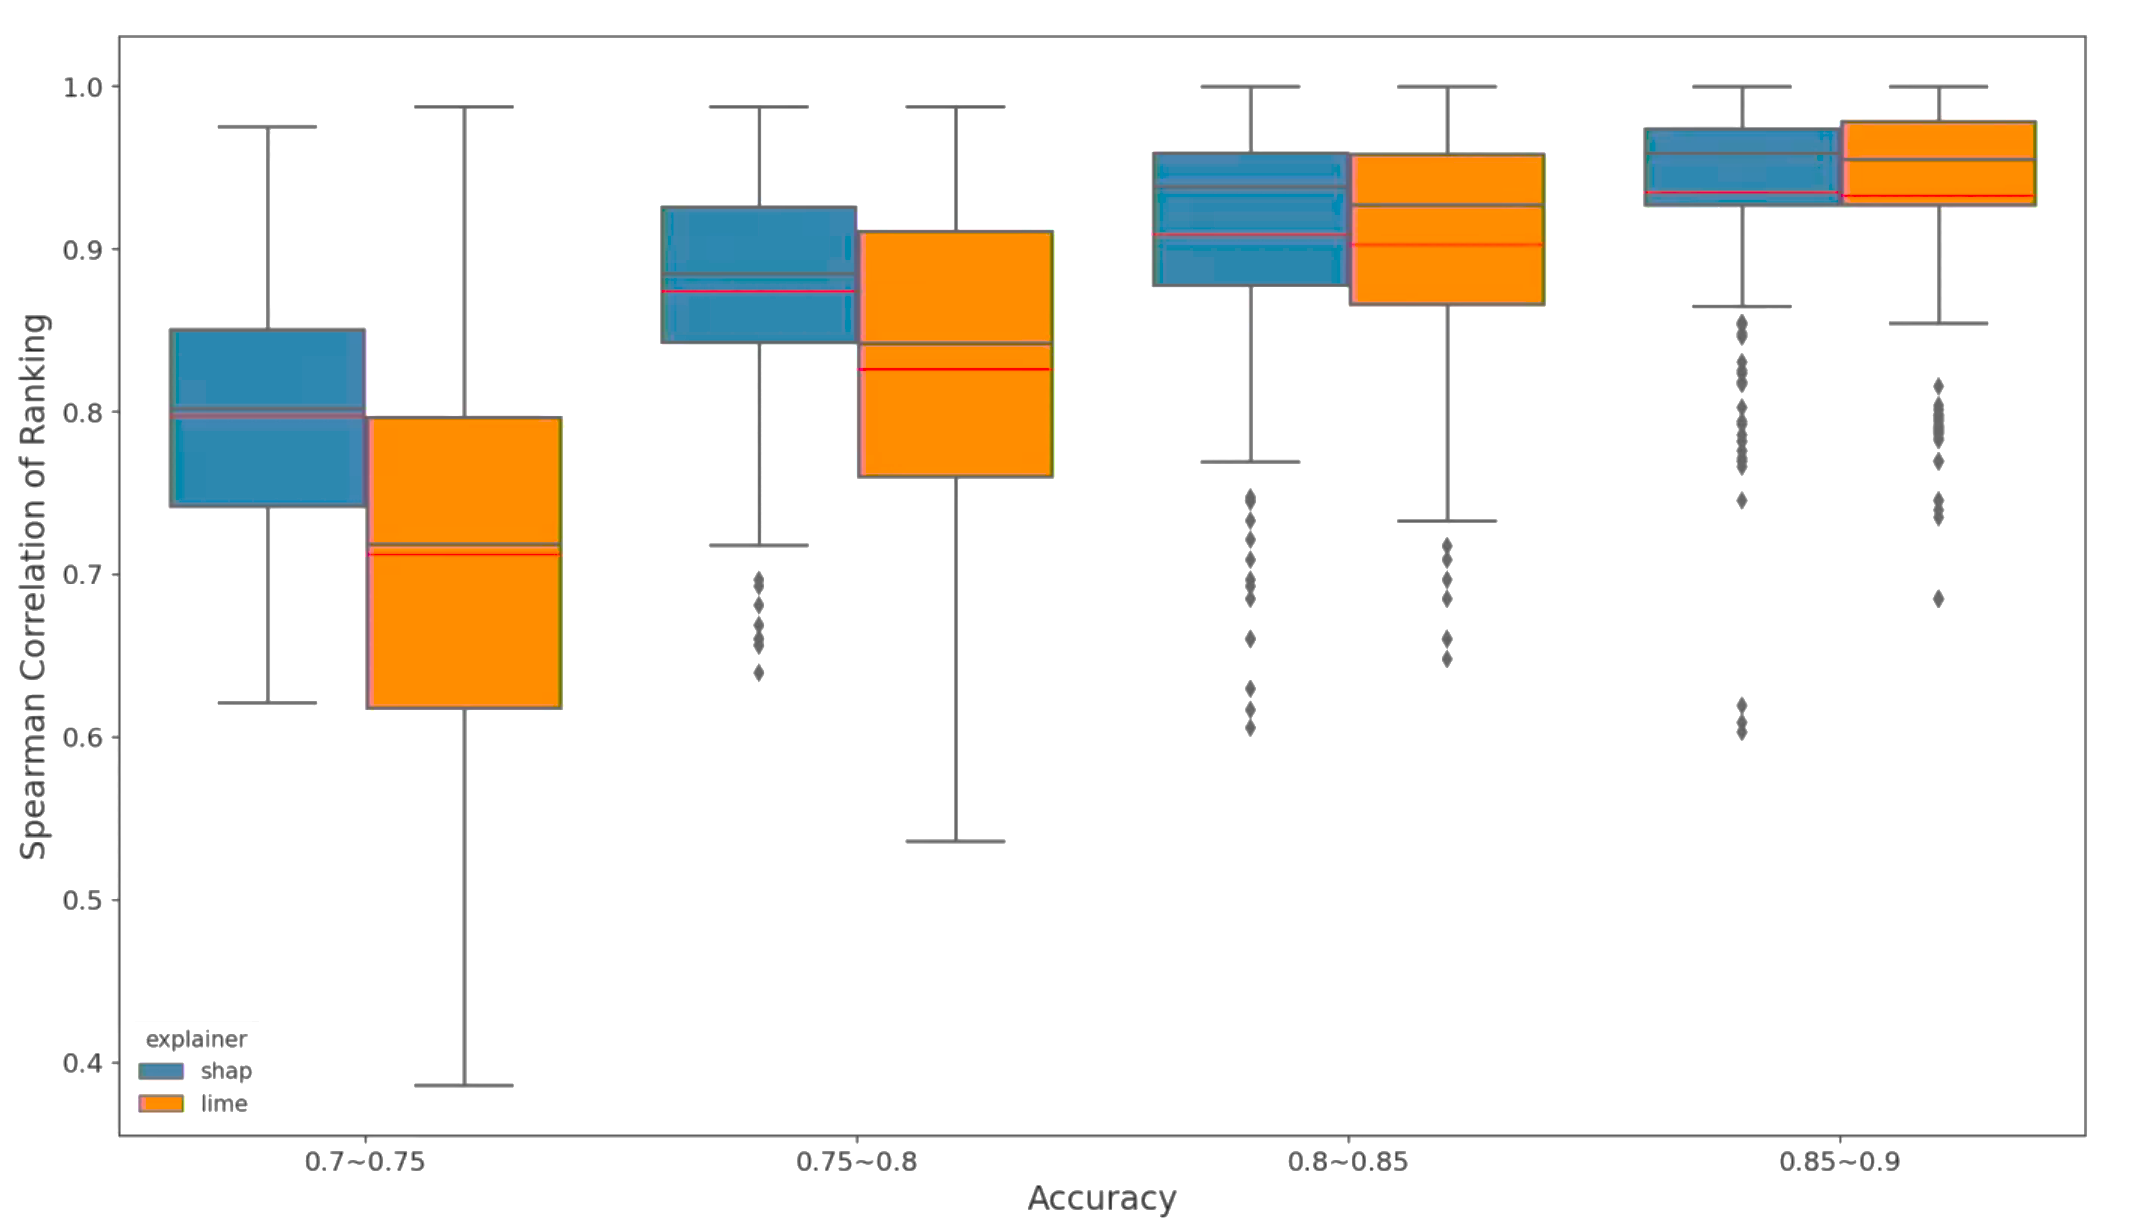
\includegraphics[width=0.45\textwidth]{media/image1.png}
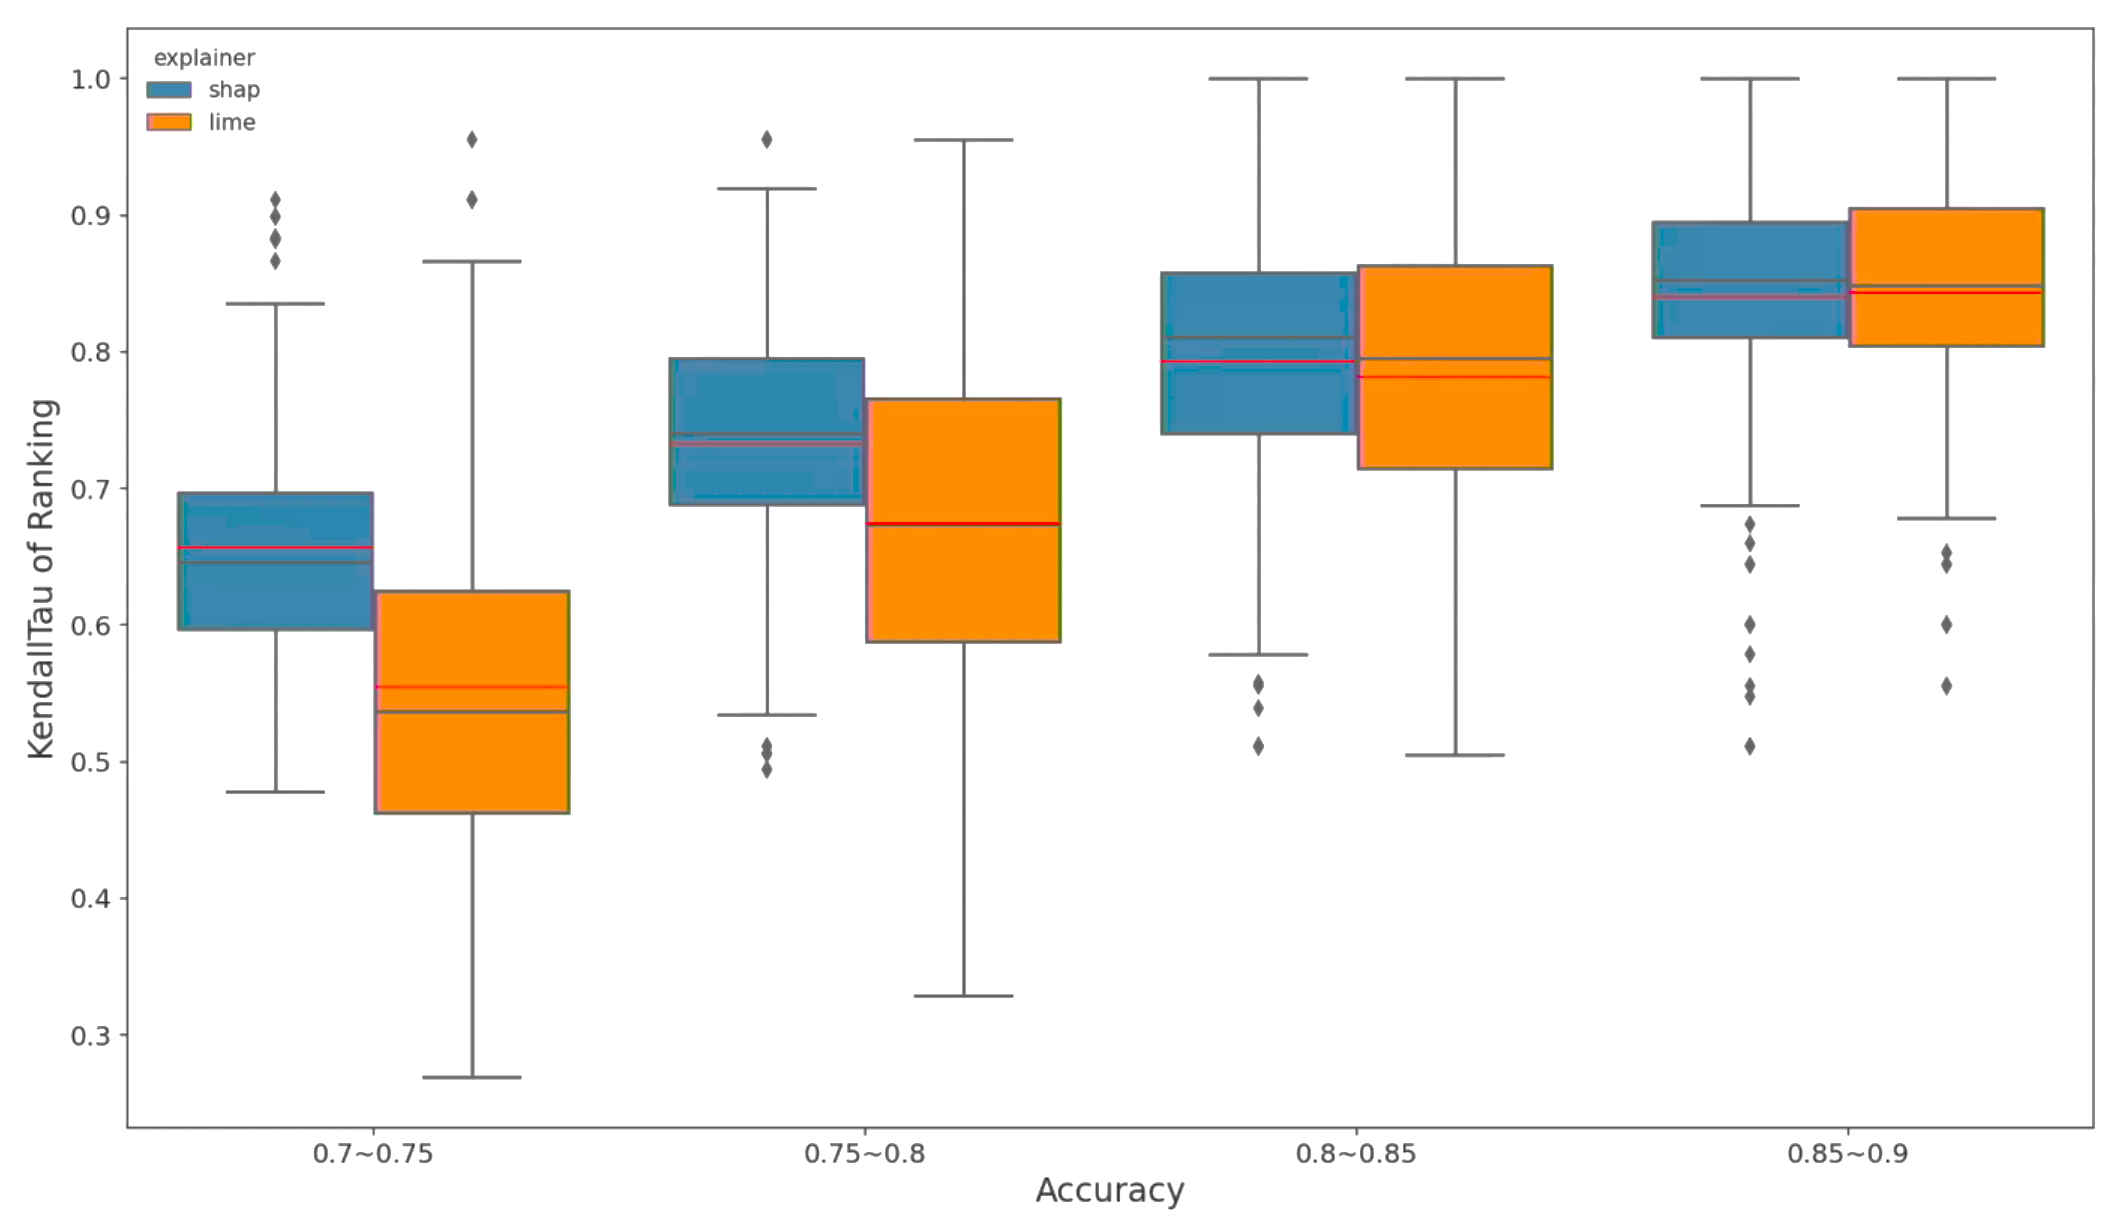
\includegraphics[width=0.45\textwidth]{media/image2.png}
\caption{Fig 1.1 Global Spearman Correlation of Explanations (LIME/SHAP) Ranking Between M and G Under Different Accuracy Levels (left) and Fig 1.2. Global Kendall Tau of Explanations (LIME/SHAP) Ranking Between M and G Under Different Accuracy Levels (right)}
\end{figure}

\begin{figure}[H]
\centering
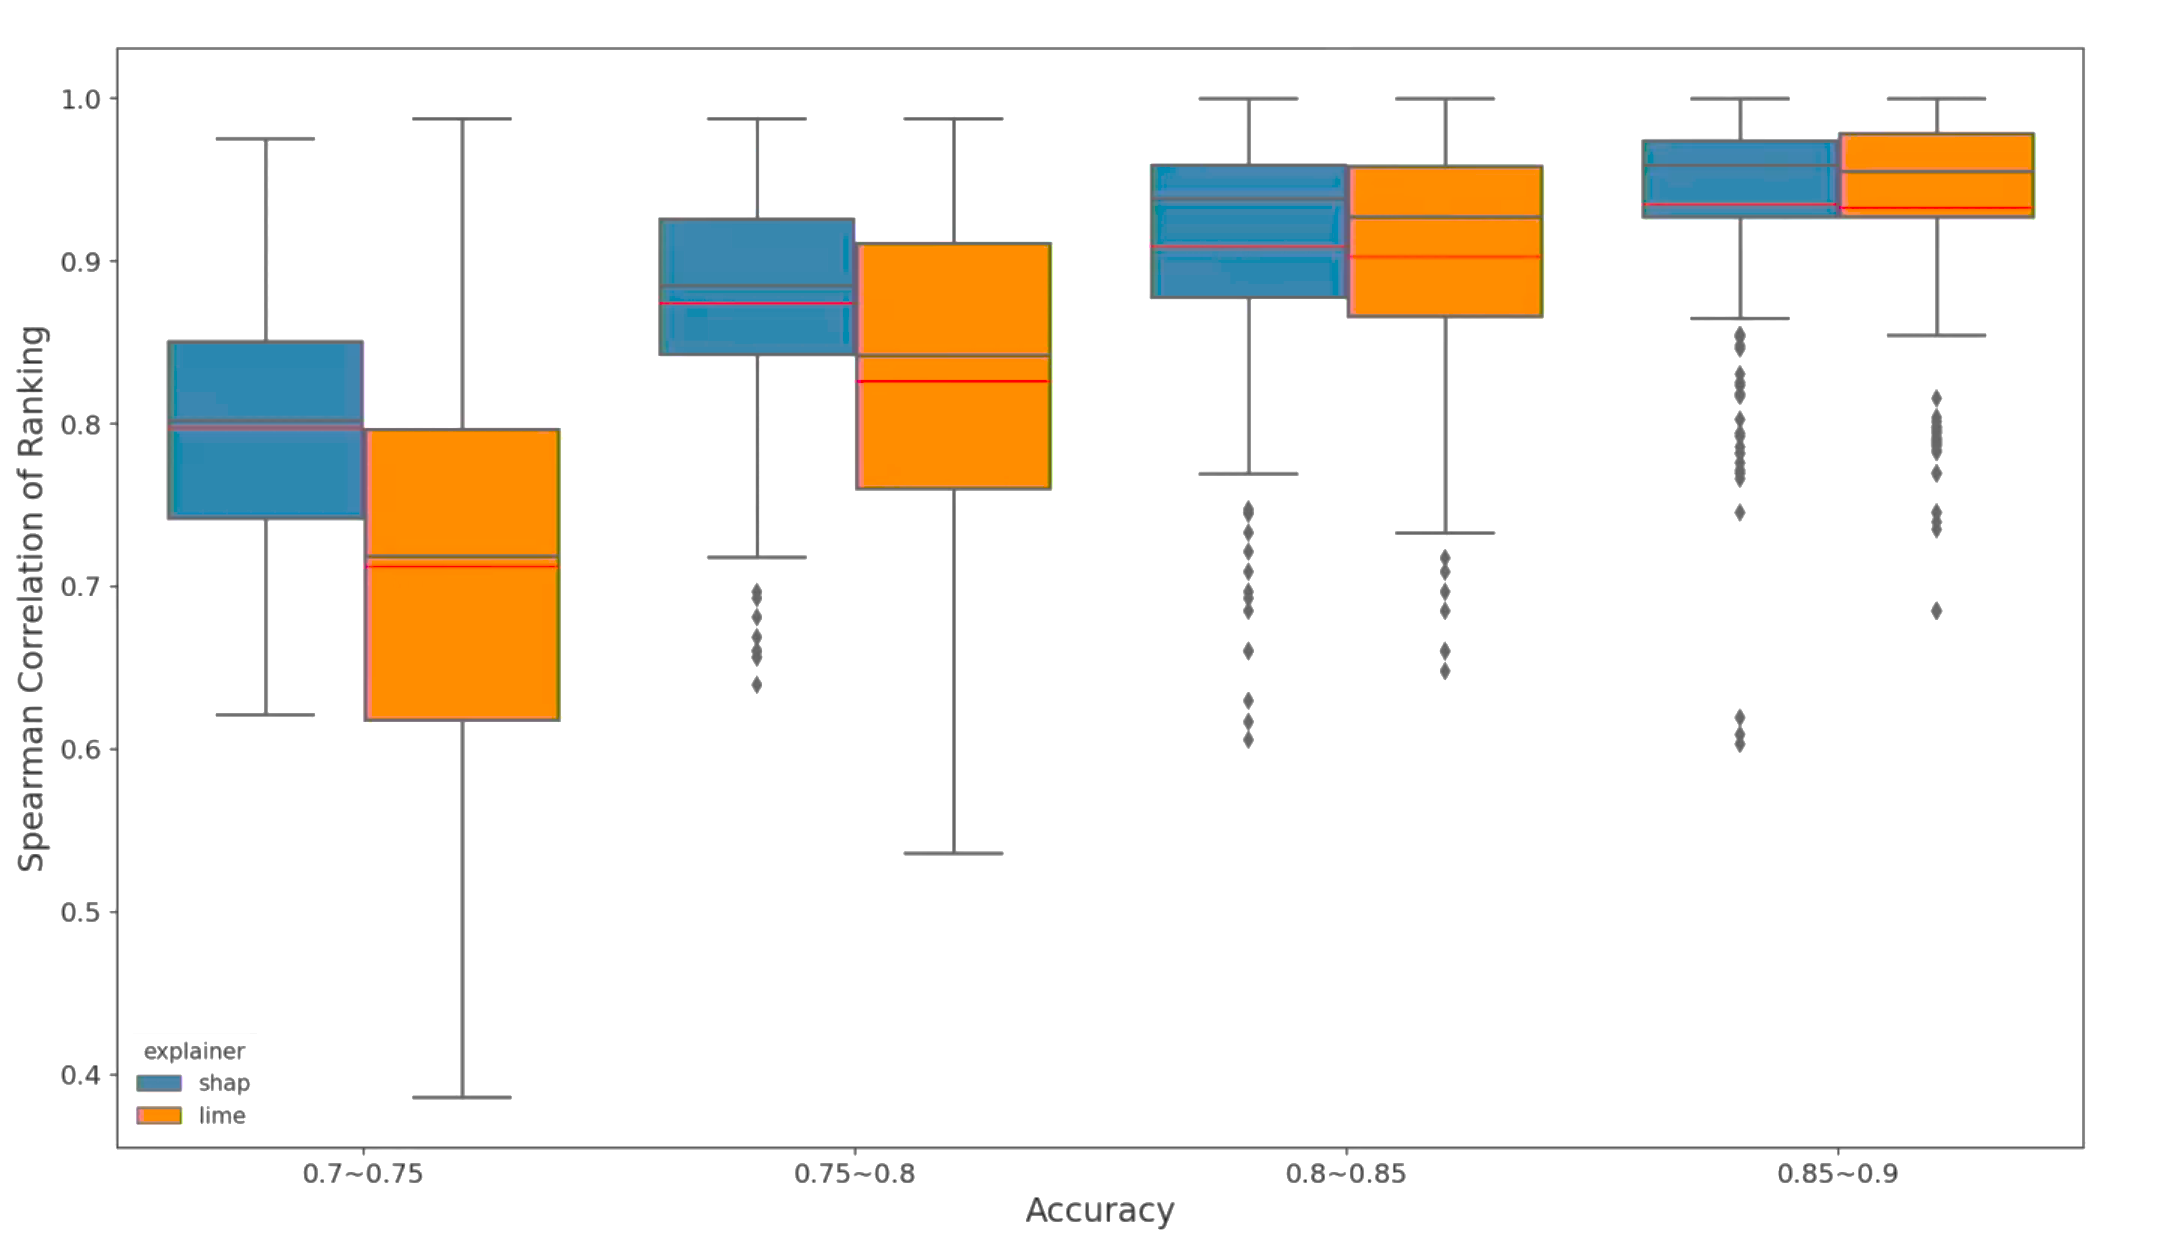
\includegraphics[width=0.45\textwidth]{media/image3.png}
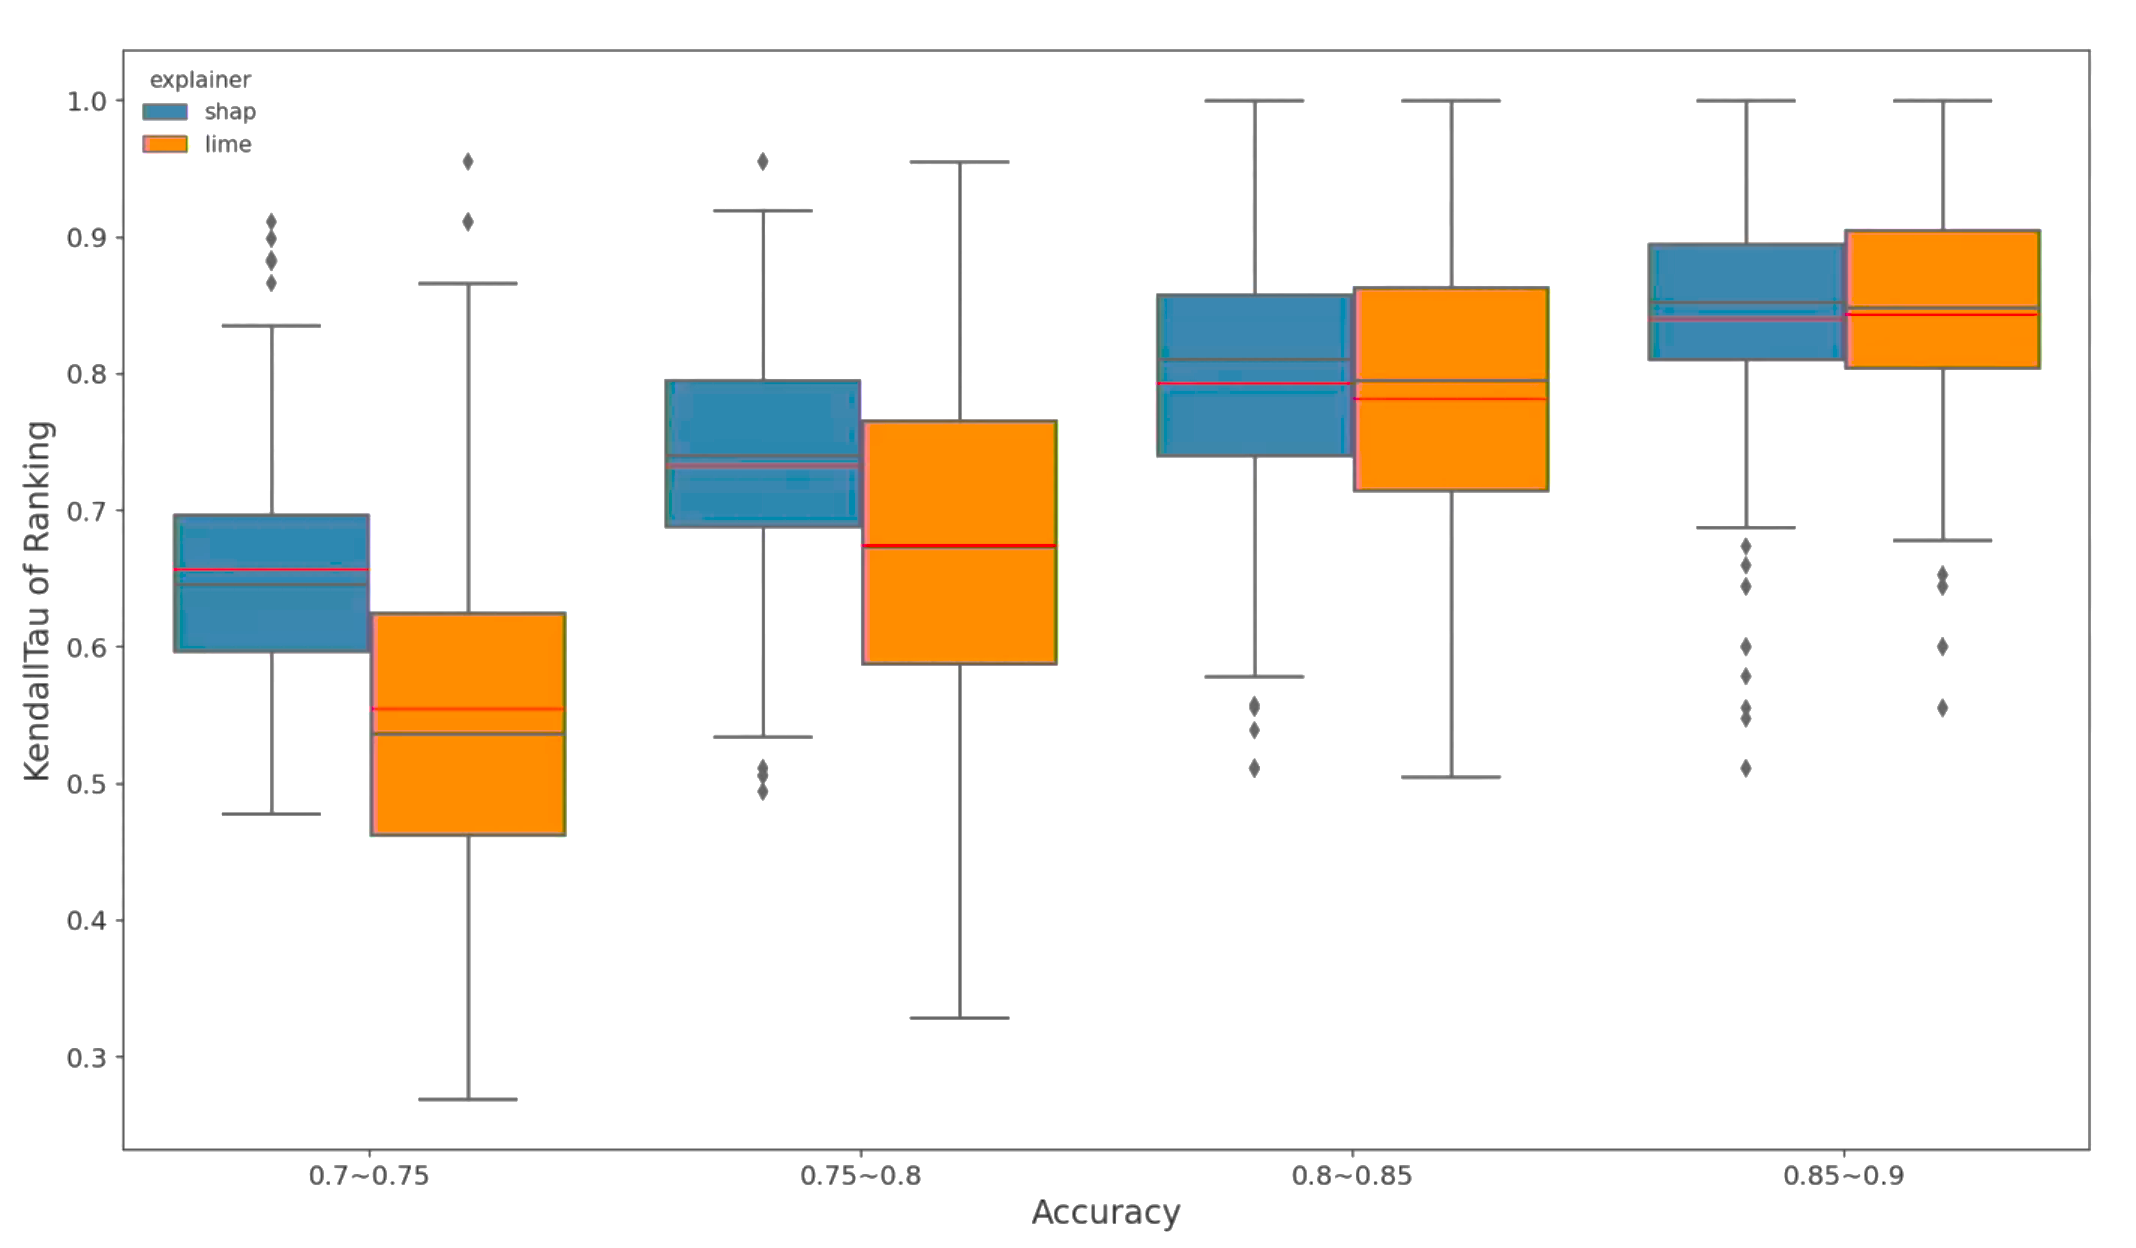
\includegraphics[width=0.45\textwidth]{media/image4.png}
\caption{Fig 2.1 Local Spearman Correlation of Explanations (LIME/SHAP) Ranking Between M and G Under Different Accuracy Levels (left) and Fig 2.2. Local Kendall Tau of Explanations (LIME/SHAP) Ranking Between M and G Under Different Accuracy Levels (right)}
\end{figure}

\begin{figure}[H]
\centering
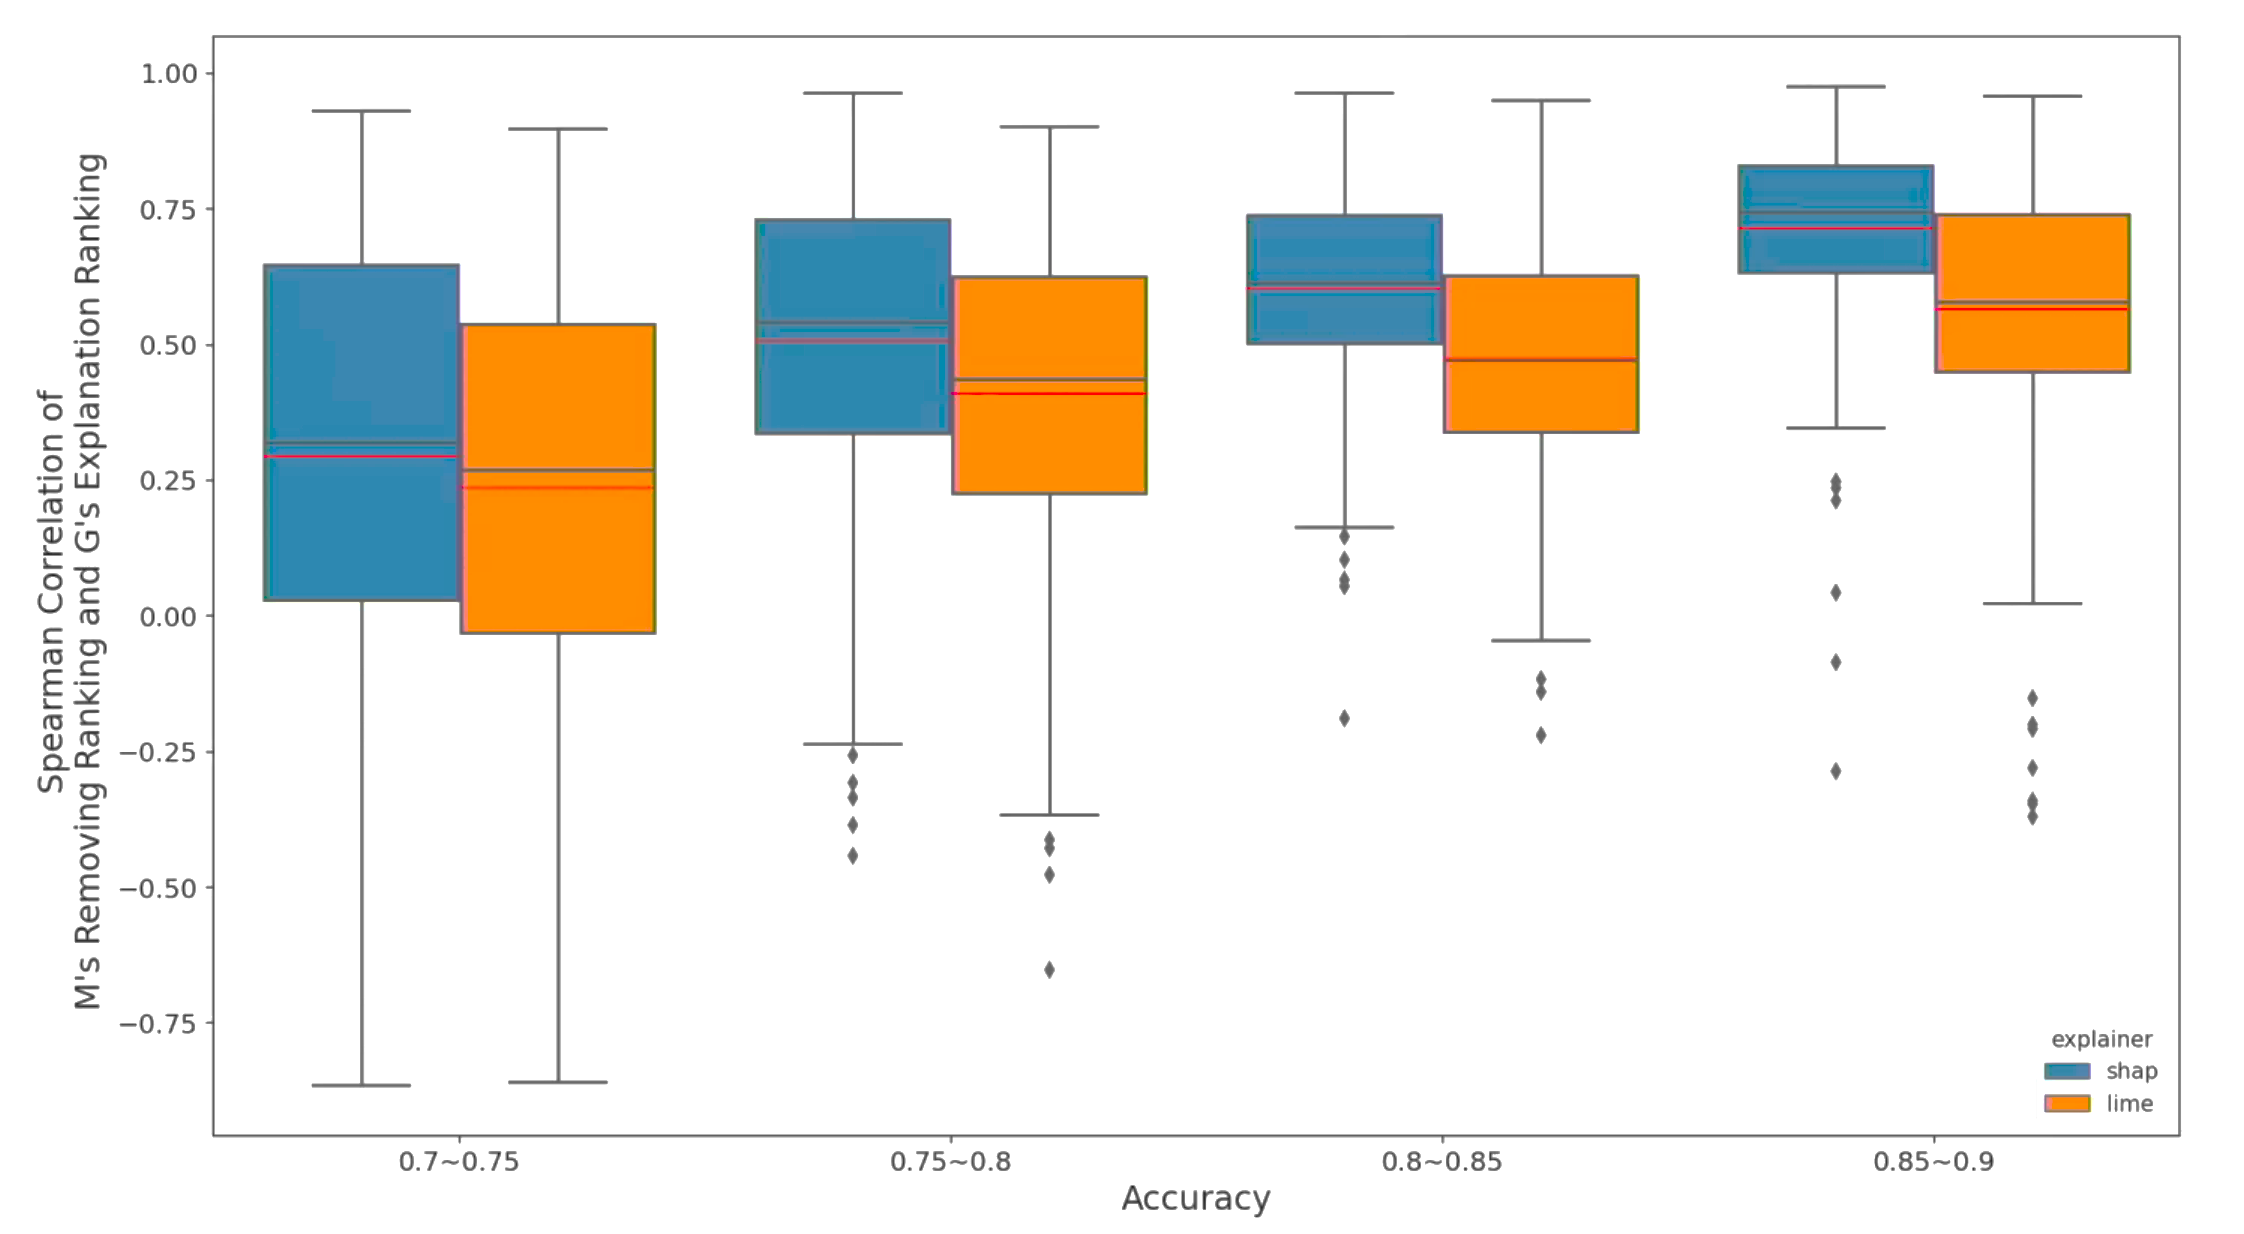
\includegraphics[width=0.45\textwidth]{media/image5.png}
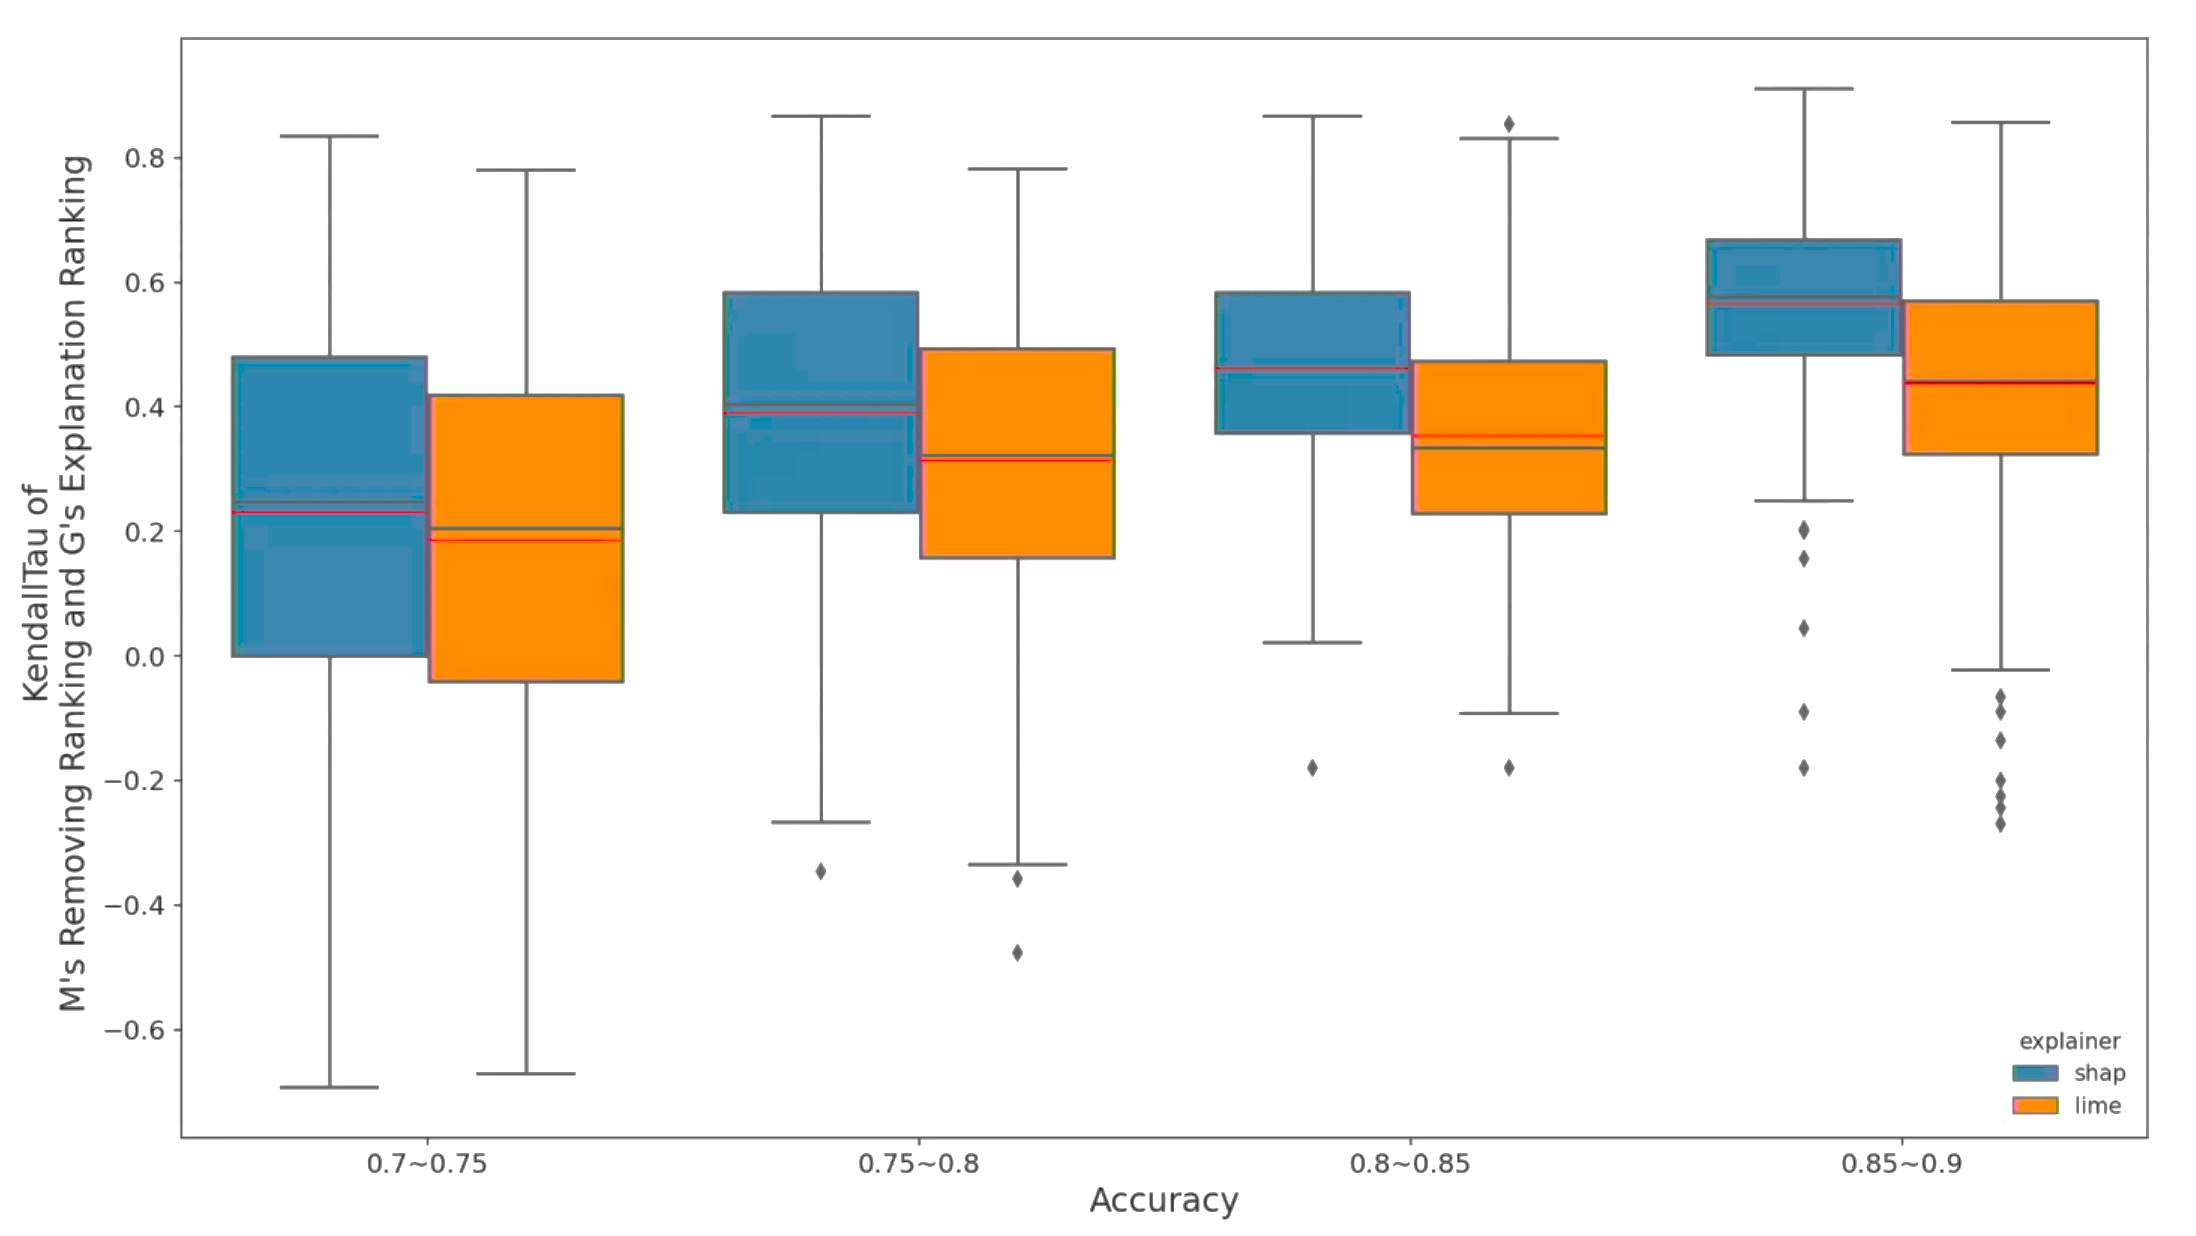
\includegraphics[width=0.45\textwidth]{media/image6.png}
\caption{Fig 3.1 Remove Ranking Spearman Correlation of Explanations (LIME/SHAP) Ranking Between M and G Under Different Accuracy Levels (left) and Fig 3.2. Remove Ranking Kendall Tau of Explanations (LIME/SHAP) Ranking Between M and G Under Different Accuracy Levels (right)}
\end{figure}

\begin{figure}[H]
\centering
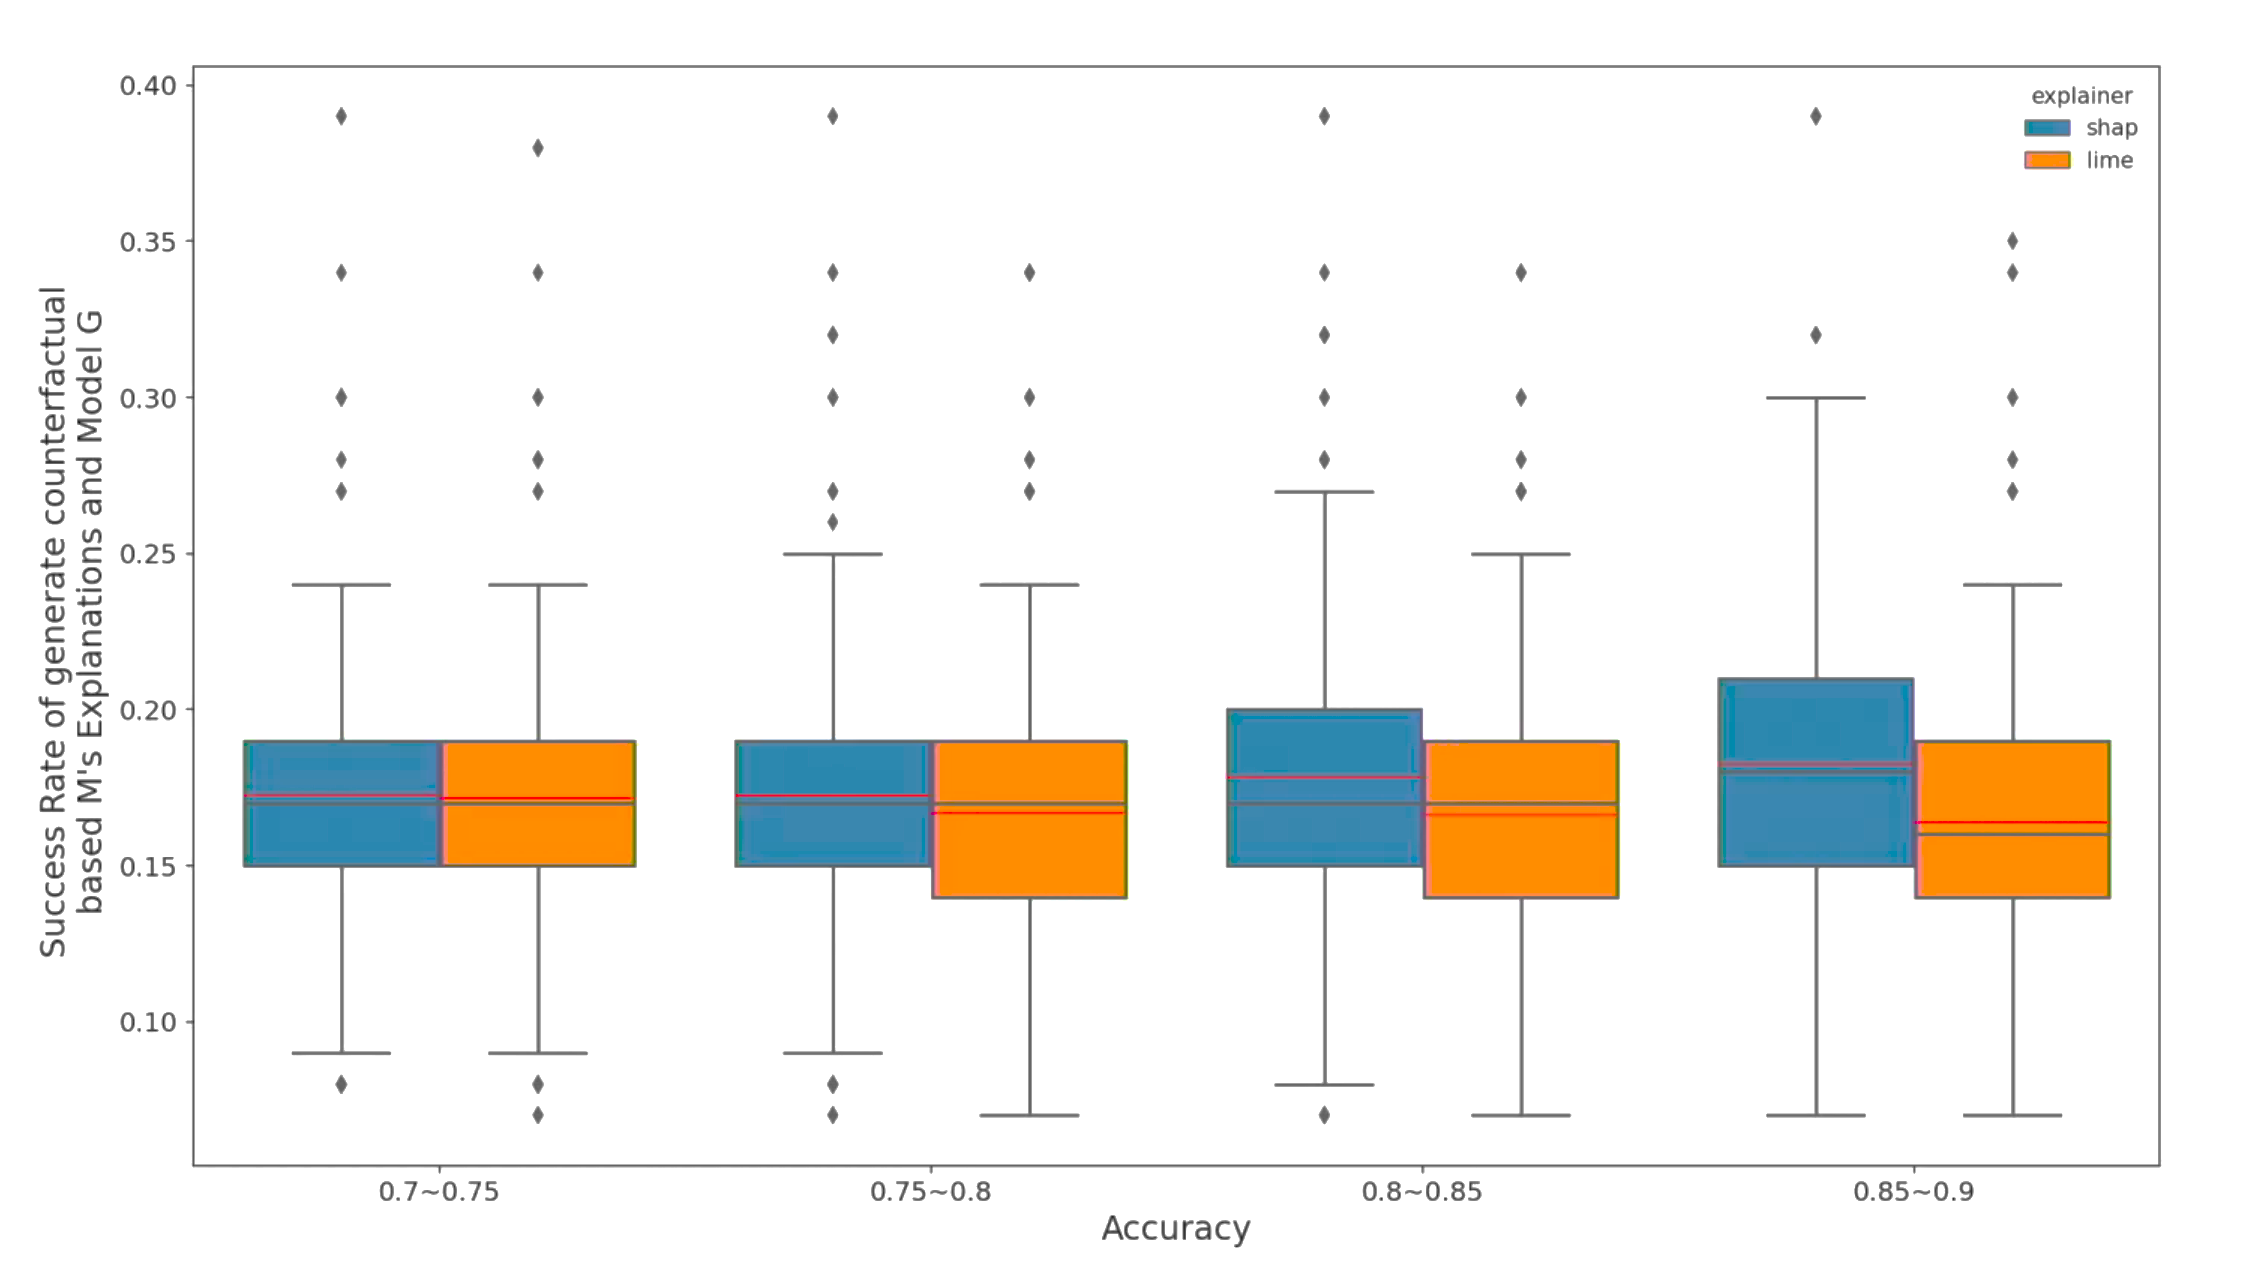
\includegraphics[width=0.7\textwidth]{media/image7.png}
\caption{Success Rate of Generate Counterfactual based M's Explanations (LIME/SHAP) and Model G Under Different Accuracy Levels}
\end{figure}

\begin{figure}[H]
\centering
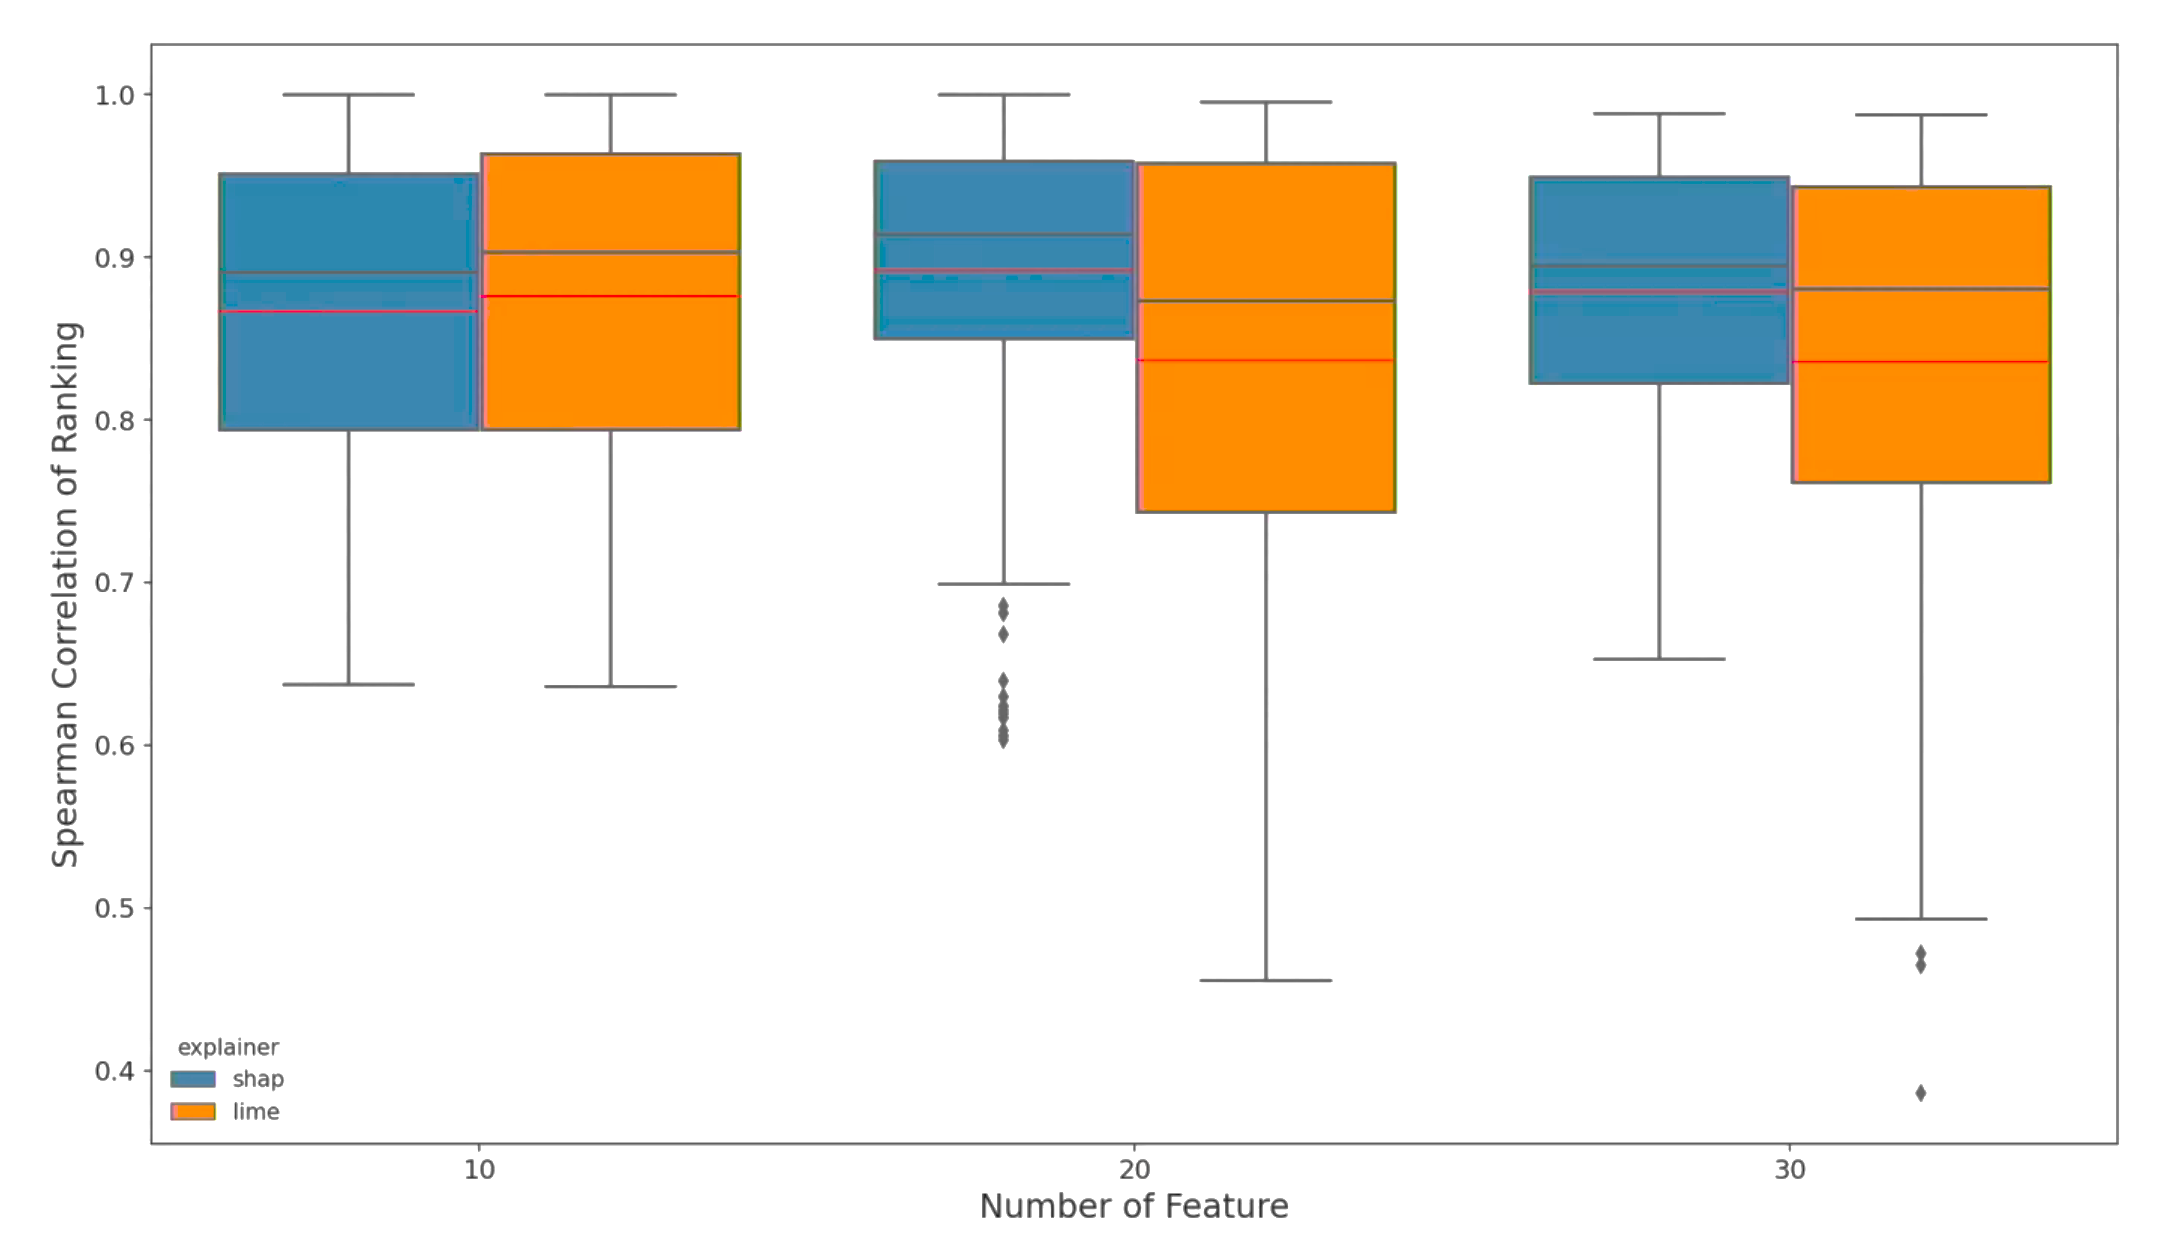
\includegraphics[width=0.45\textwidth]{media/image8.png}
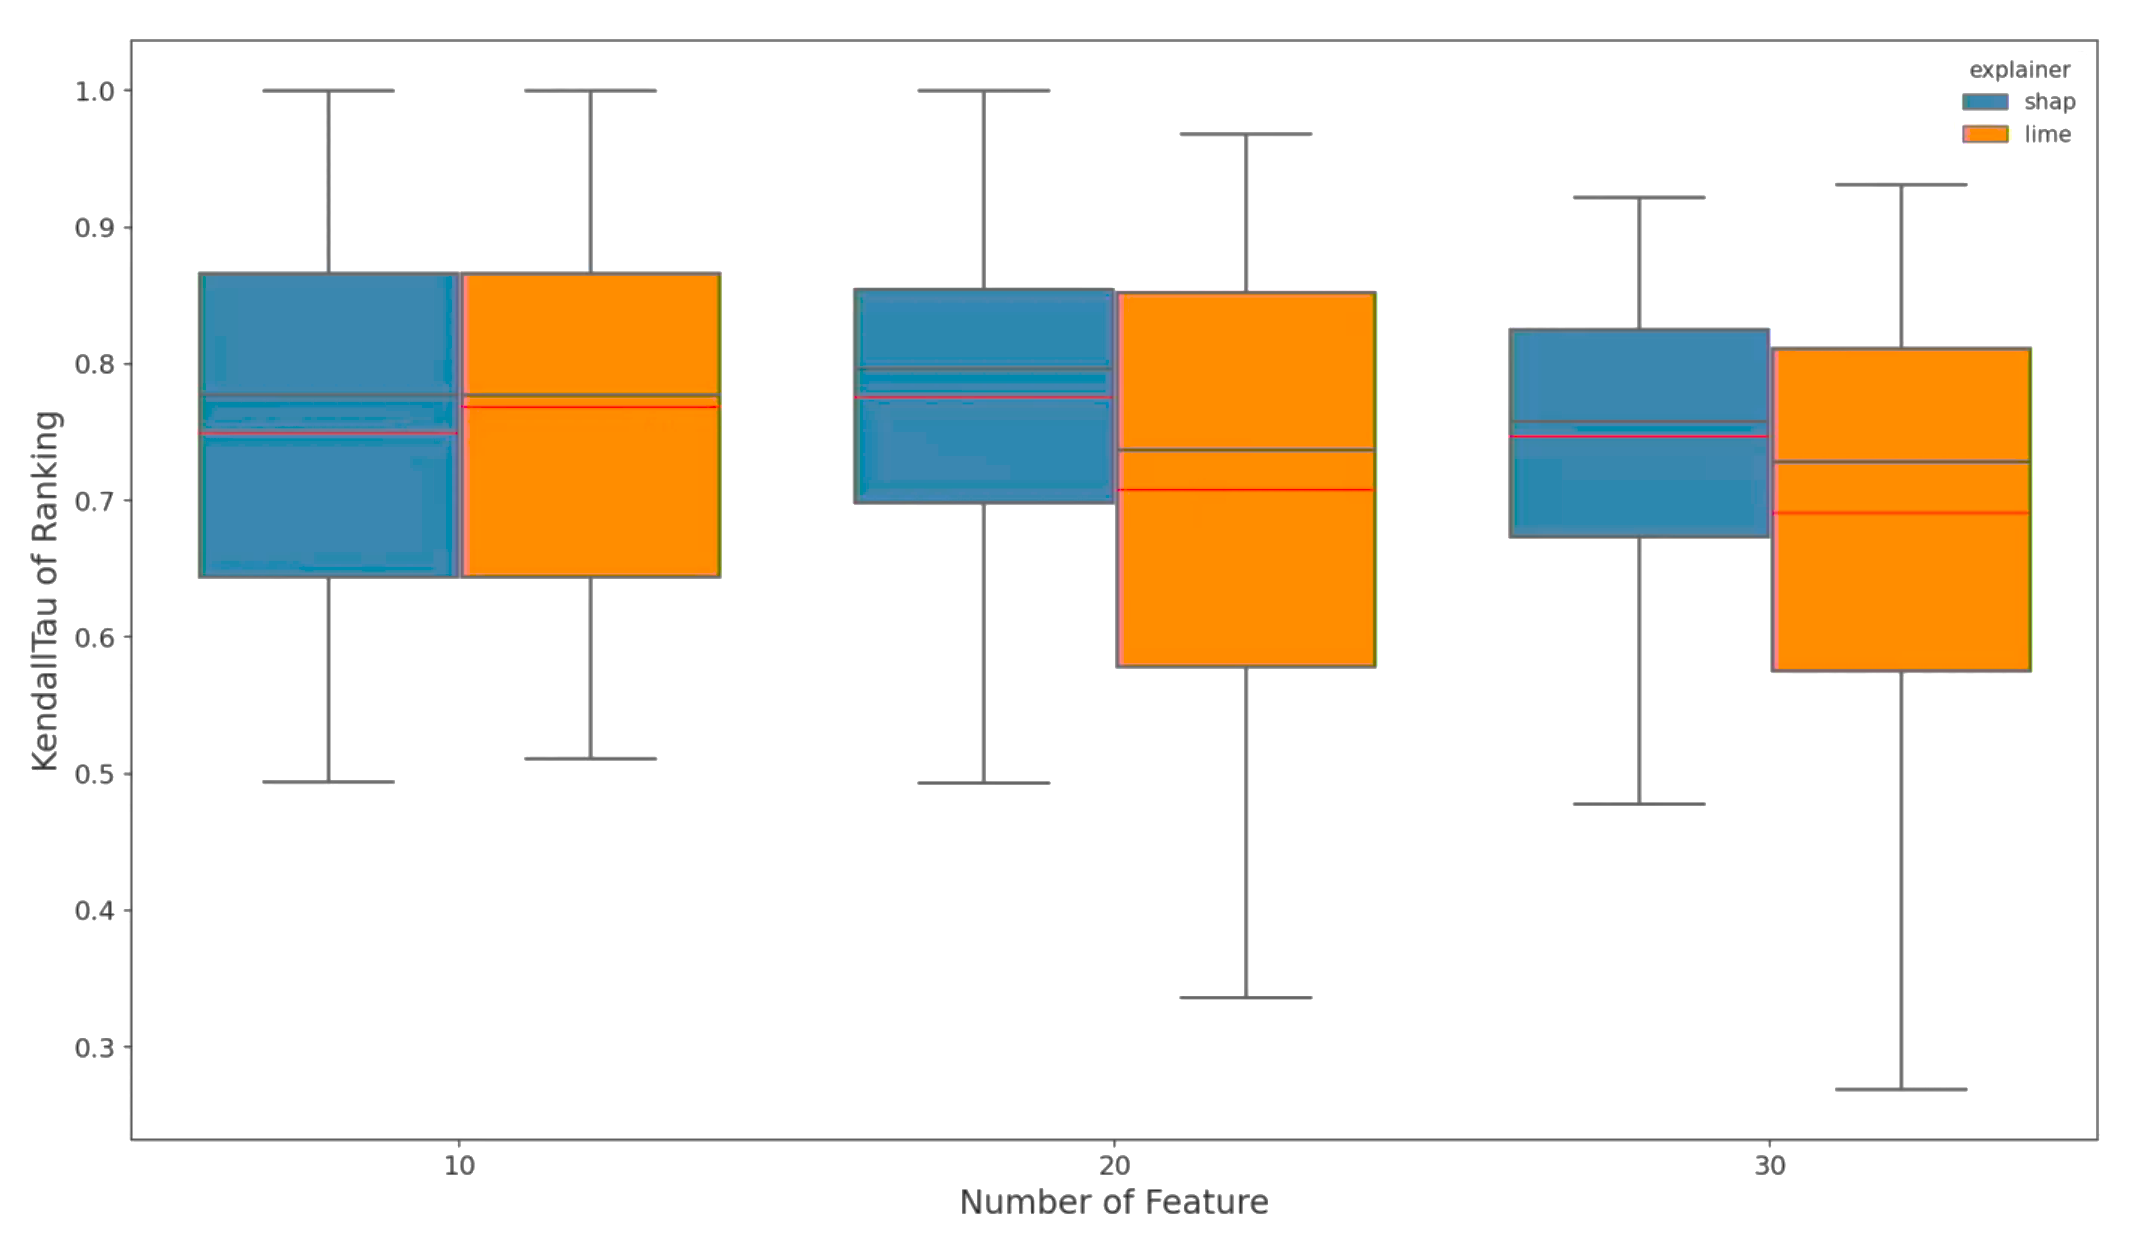
\includegraphics[width=0.45\textwidth]{media/image9.png}
\caption{Fig 5.1 Global Spearman Correlation of Explanations (LIME/SHAP) Ranking Between M and G Under Different Number of Feature (left) and Fig 5.2. Global Kendall Tau of Explanations (LIME/SHAP) Ranking Between M and G Under Different Number of Feature (right)}
\end{figure}

\begin{figure}[H]
\centering
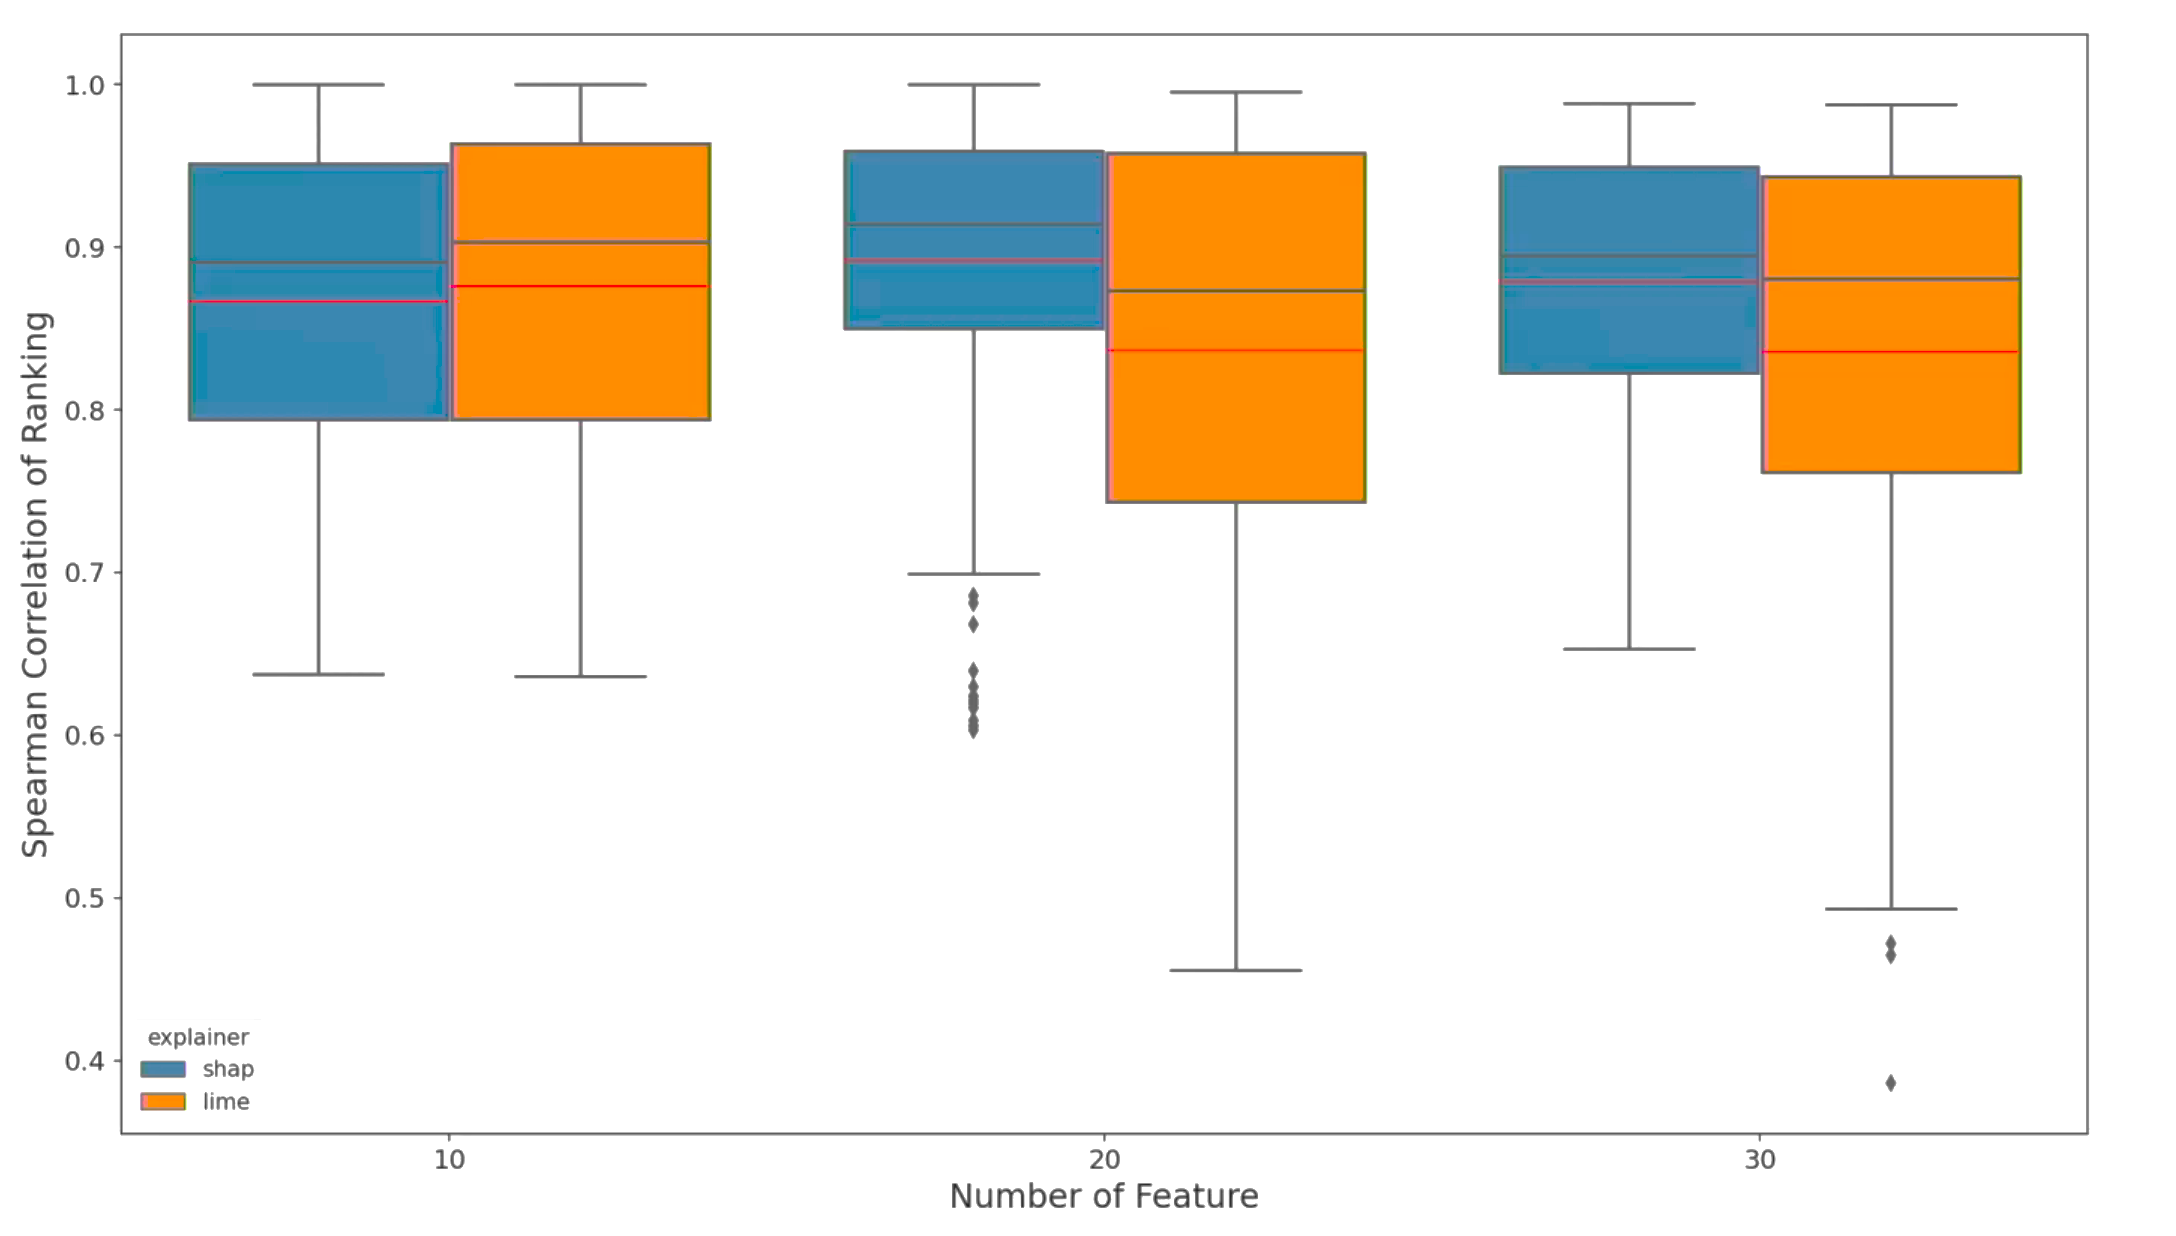
\includegraphics[width=0.45\textwidth]{media/image10.png}
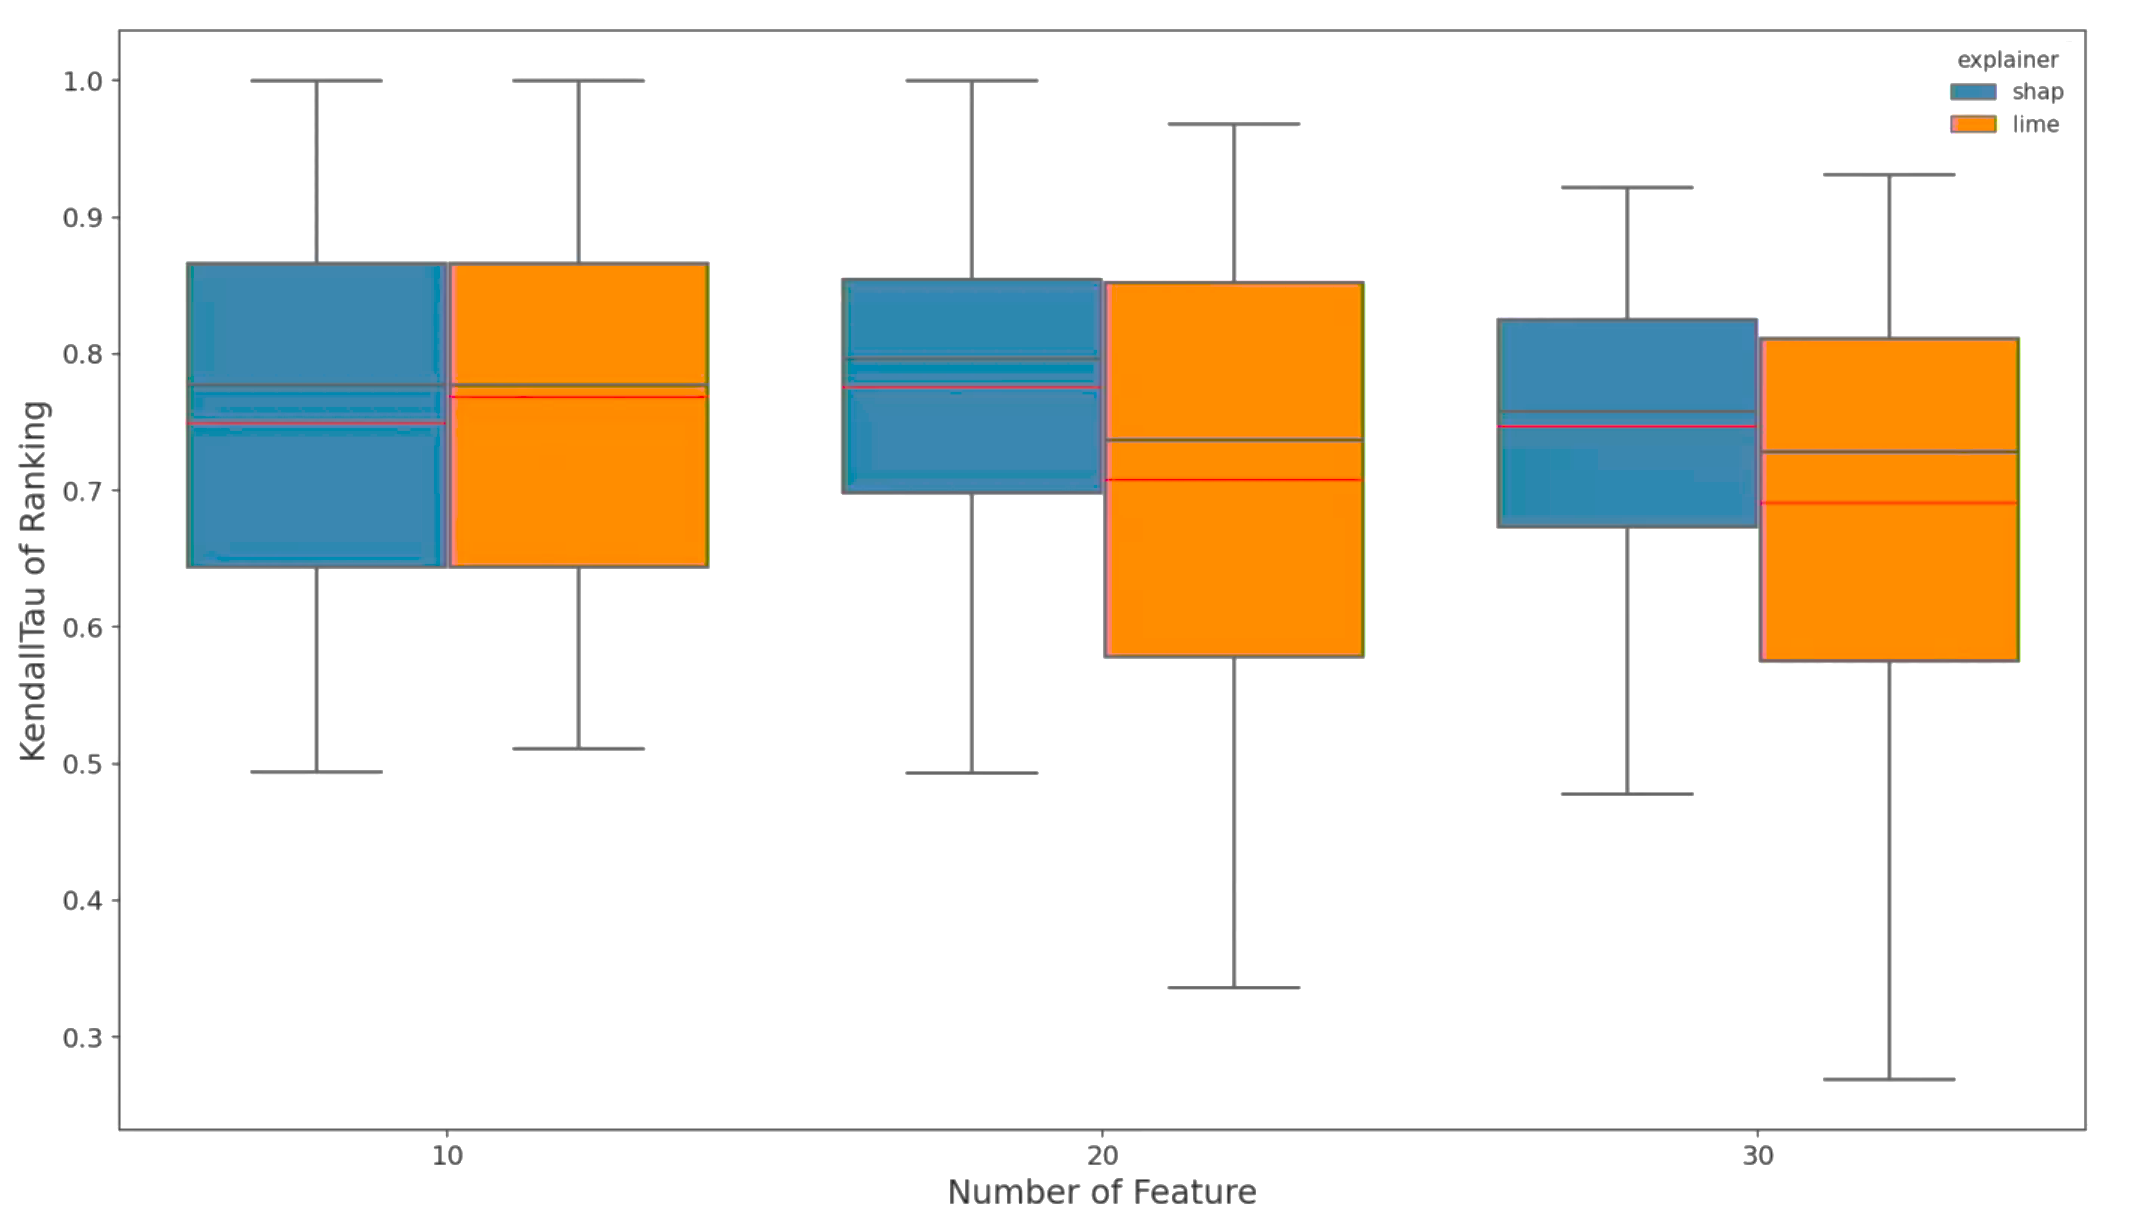
\includegraphics[width=0.45\textwidth]{media/image11.png}
\caption{Fig 6.1 Local Spearman Correlation of Explanations (LIME/SHAP) Ranking Between M and G Under Different Number of Feature (left) and Fig 6.2. Local Kendall Tau of Explanations (LIME/SHAP) Ranking Between M and G Under Different Number of Feature (right)}
\end{figure}

\begin{figure}[H]
\centering
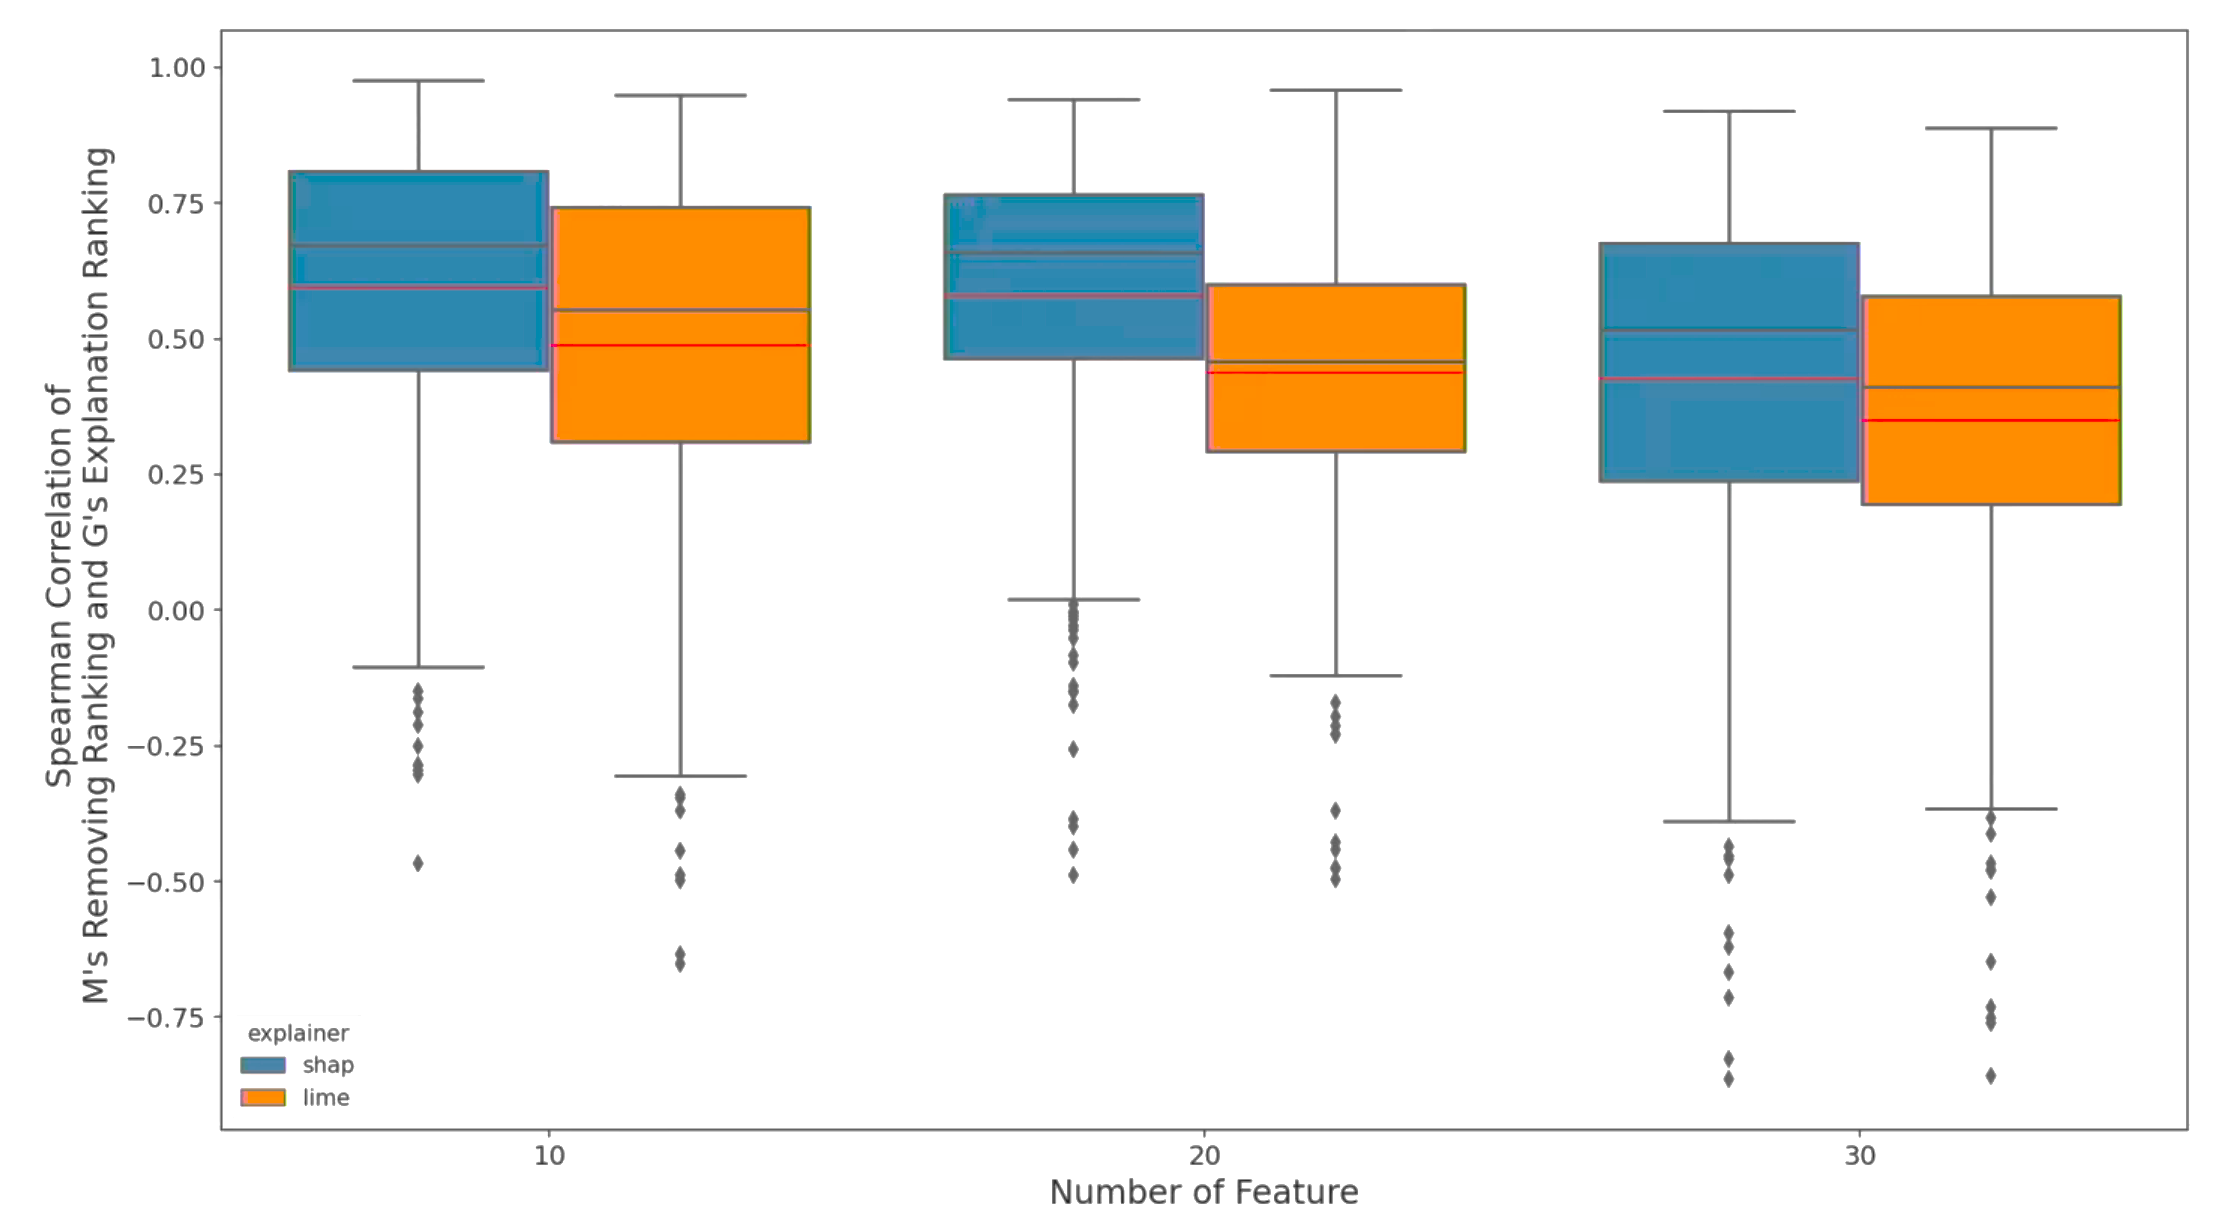
\includegraphics[width=0.45\textwidth]{media/image12.png}
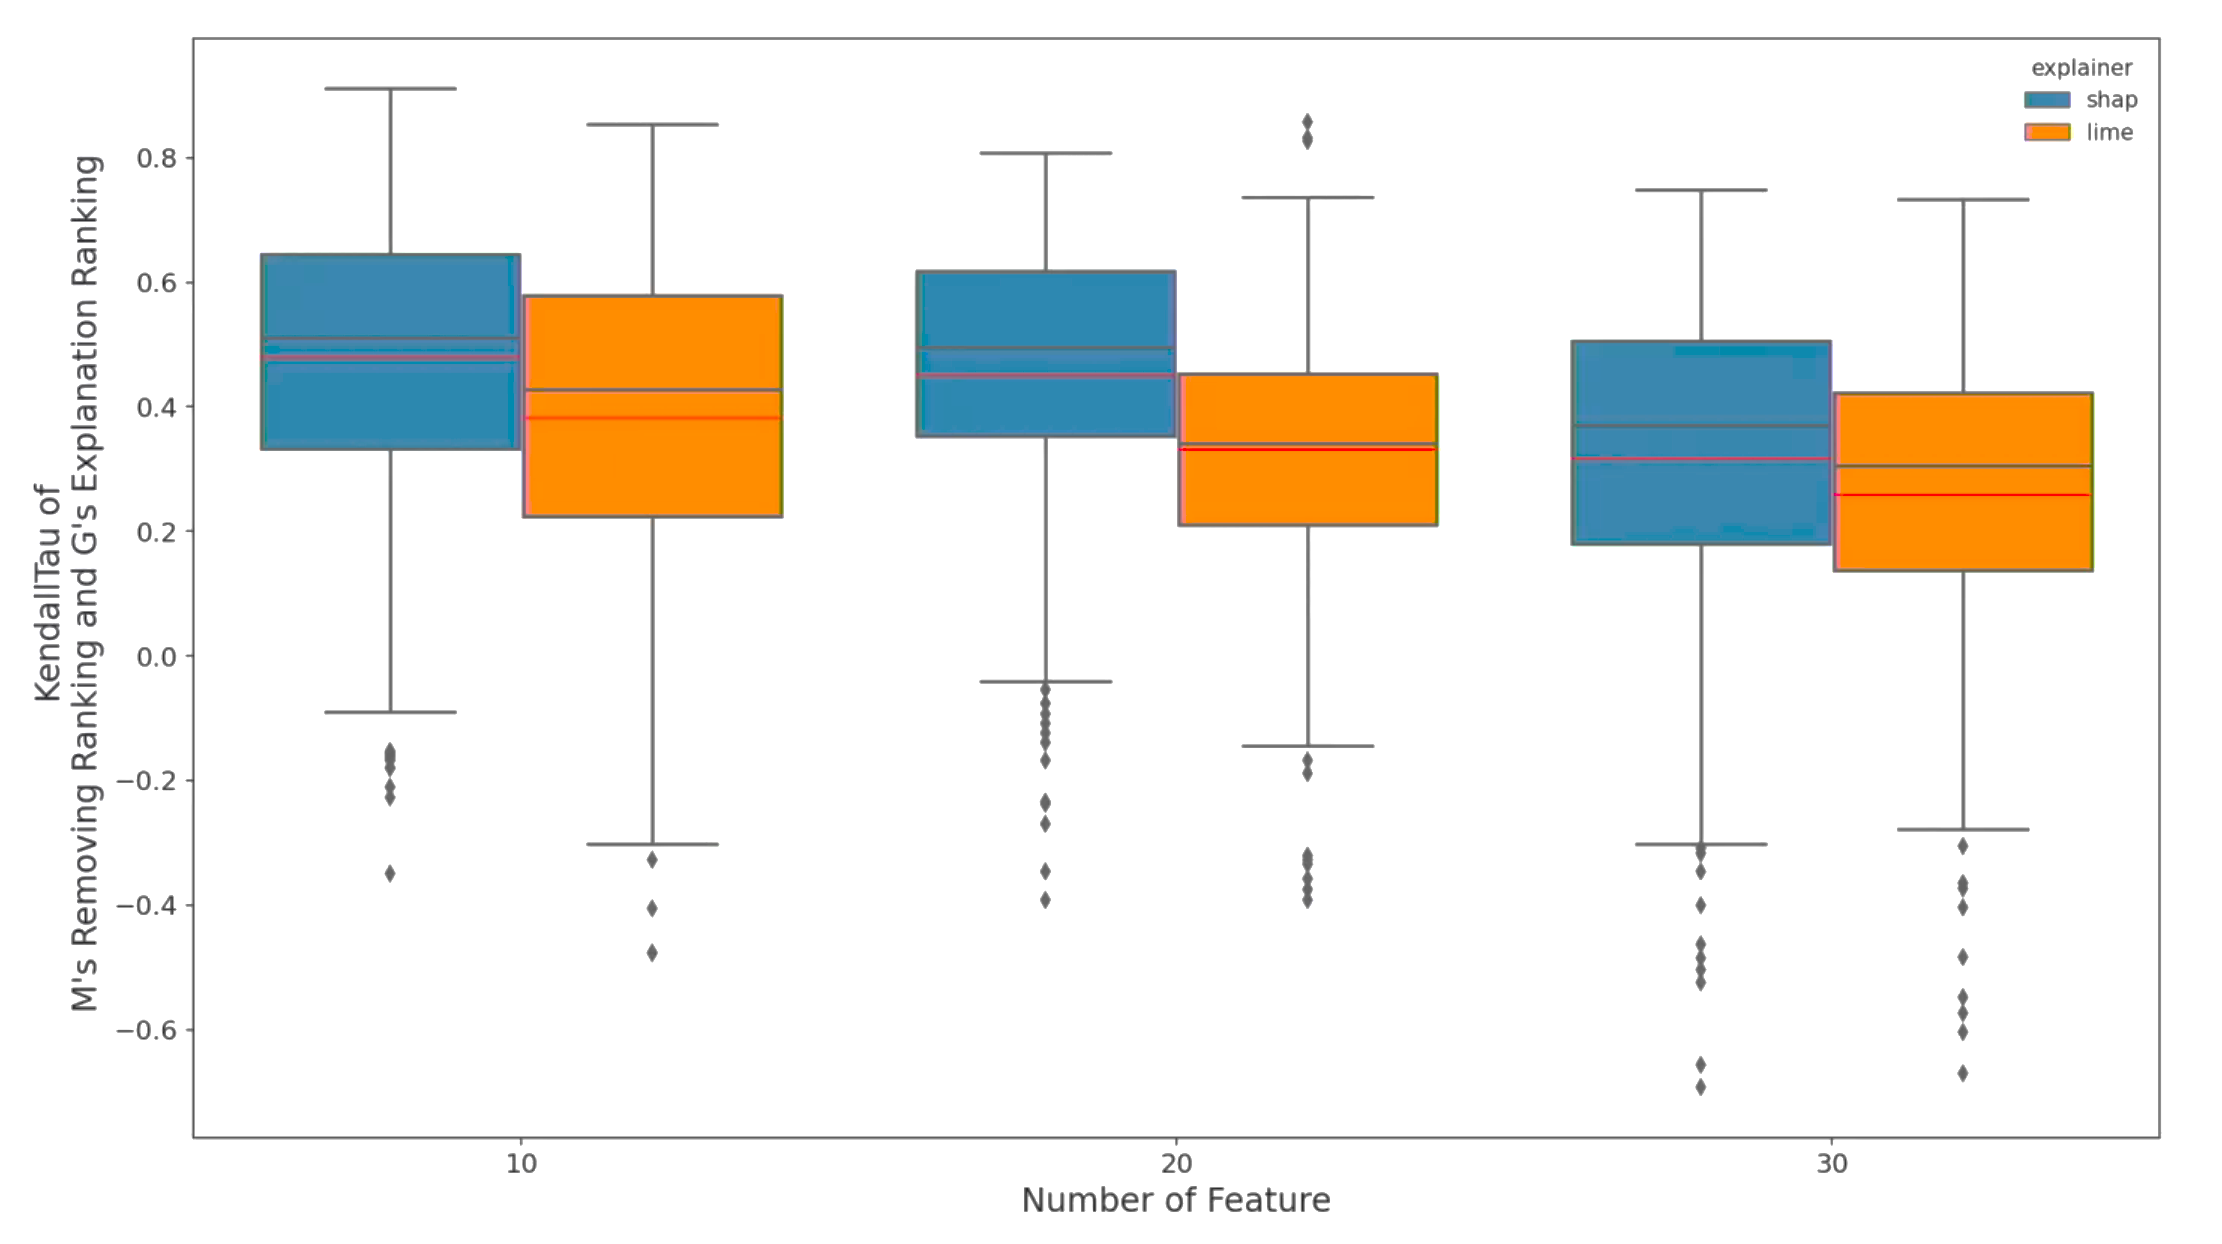
\includegraphics[width=0.45\textwidth]{media/image13.png}
\caption{Fig 7.1 Remove Ranking Spearman Correlation of Explanations (LIME/SHAP) Ranking Between M and G Under Different Number of Feature (left) and Fig 7.2. Remove Ranking Kendall Tau of Explanations (LIME/SHAP) Ranking Between M and G Under Different Number of Feature (right)}
\end{figure}

\begin{figure}[H]
\centering
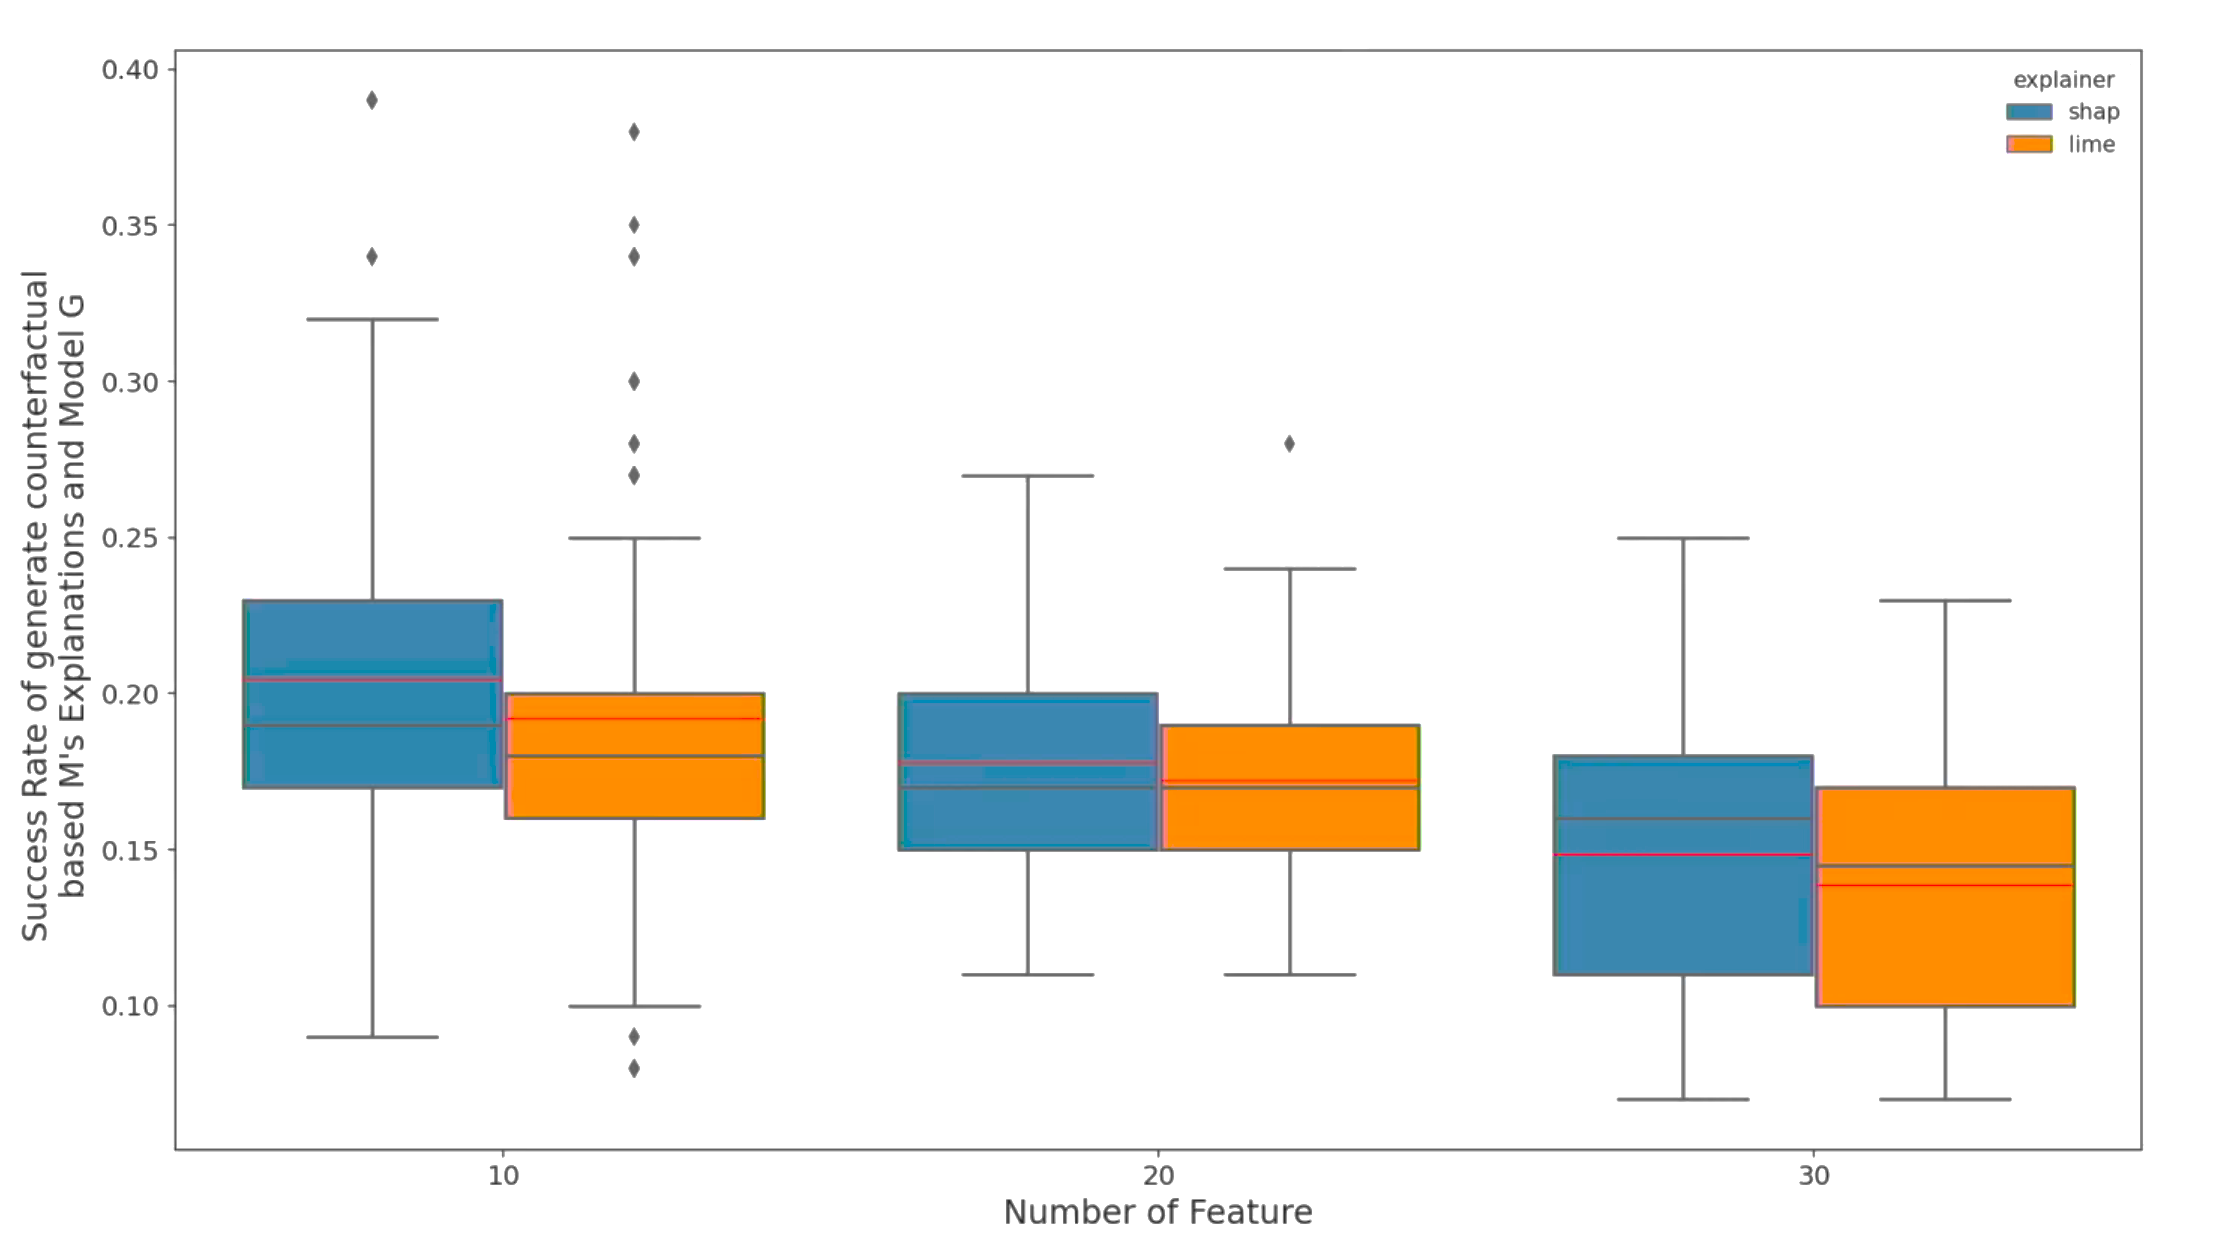
\includegraphics[width=0.7\textwidth]{media/image14.png}
\caption{Fig Success Rate of Generate Counterfactual based M's Explanations (LIME/SHAP) and Model G Under Different Number of Feature}
\end{figure}

\begin{figure}[H]
\centering
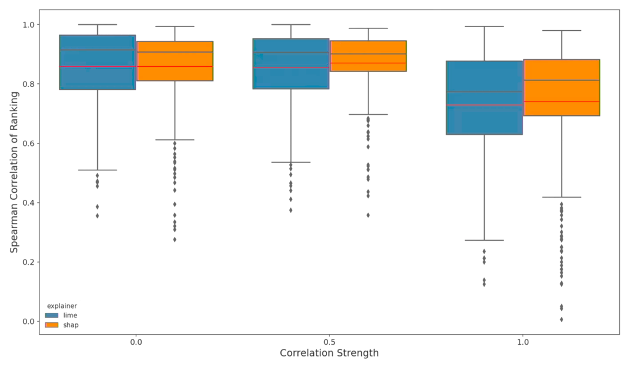
\includegraphics[width=0.45\textwidth]{media/image15.png}
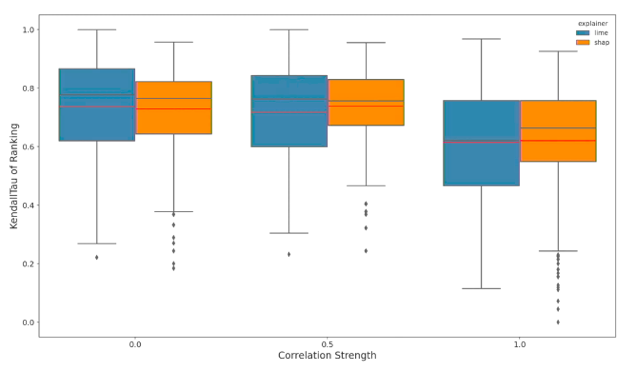
\includegraphics[width=0.45\textwidth]{media/image16.png}
\caption{Fig 9.1 Global Spearman Correlation of Explanations (LIME/SHAP) Ranking Between M and G Under Different Correlation Strength (left) and Fig 9.2. Global Kendall Tau of Explanations (LIME/SHAP) Ranking Between M and G Under Different Correlation Strength (right)}
\end{figure}

\begin{figure}[H]
\centering
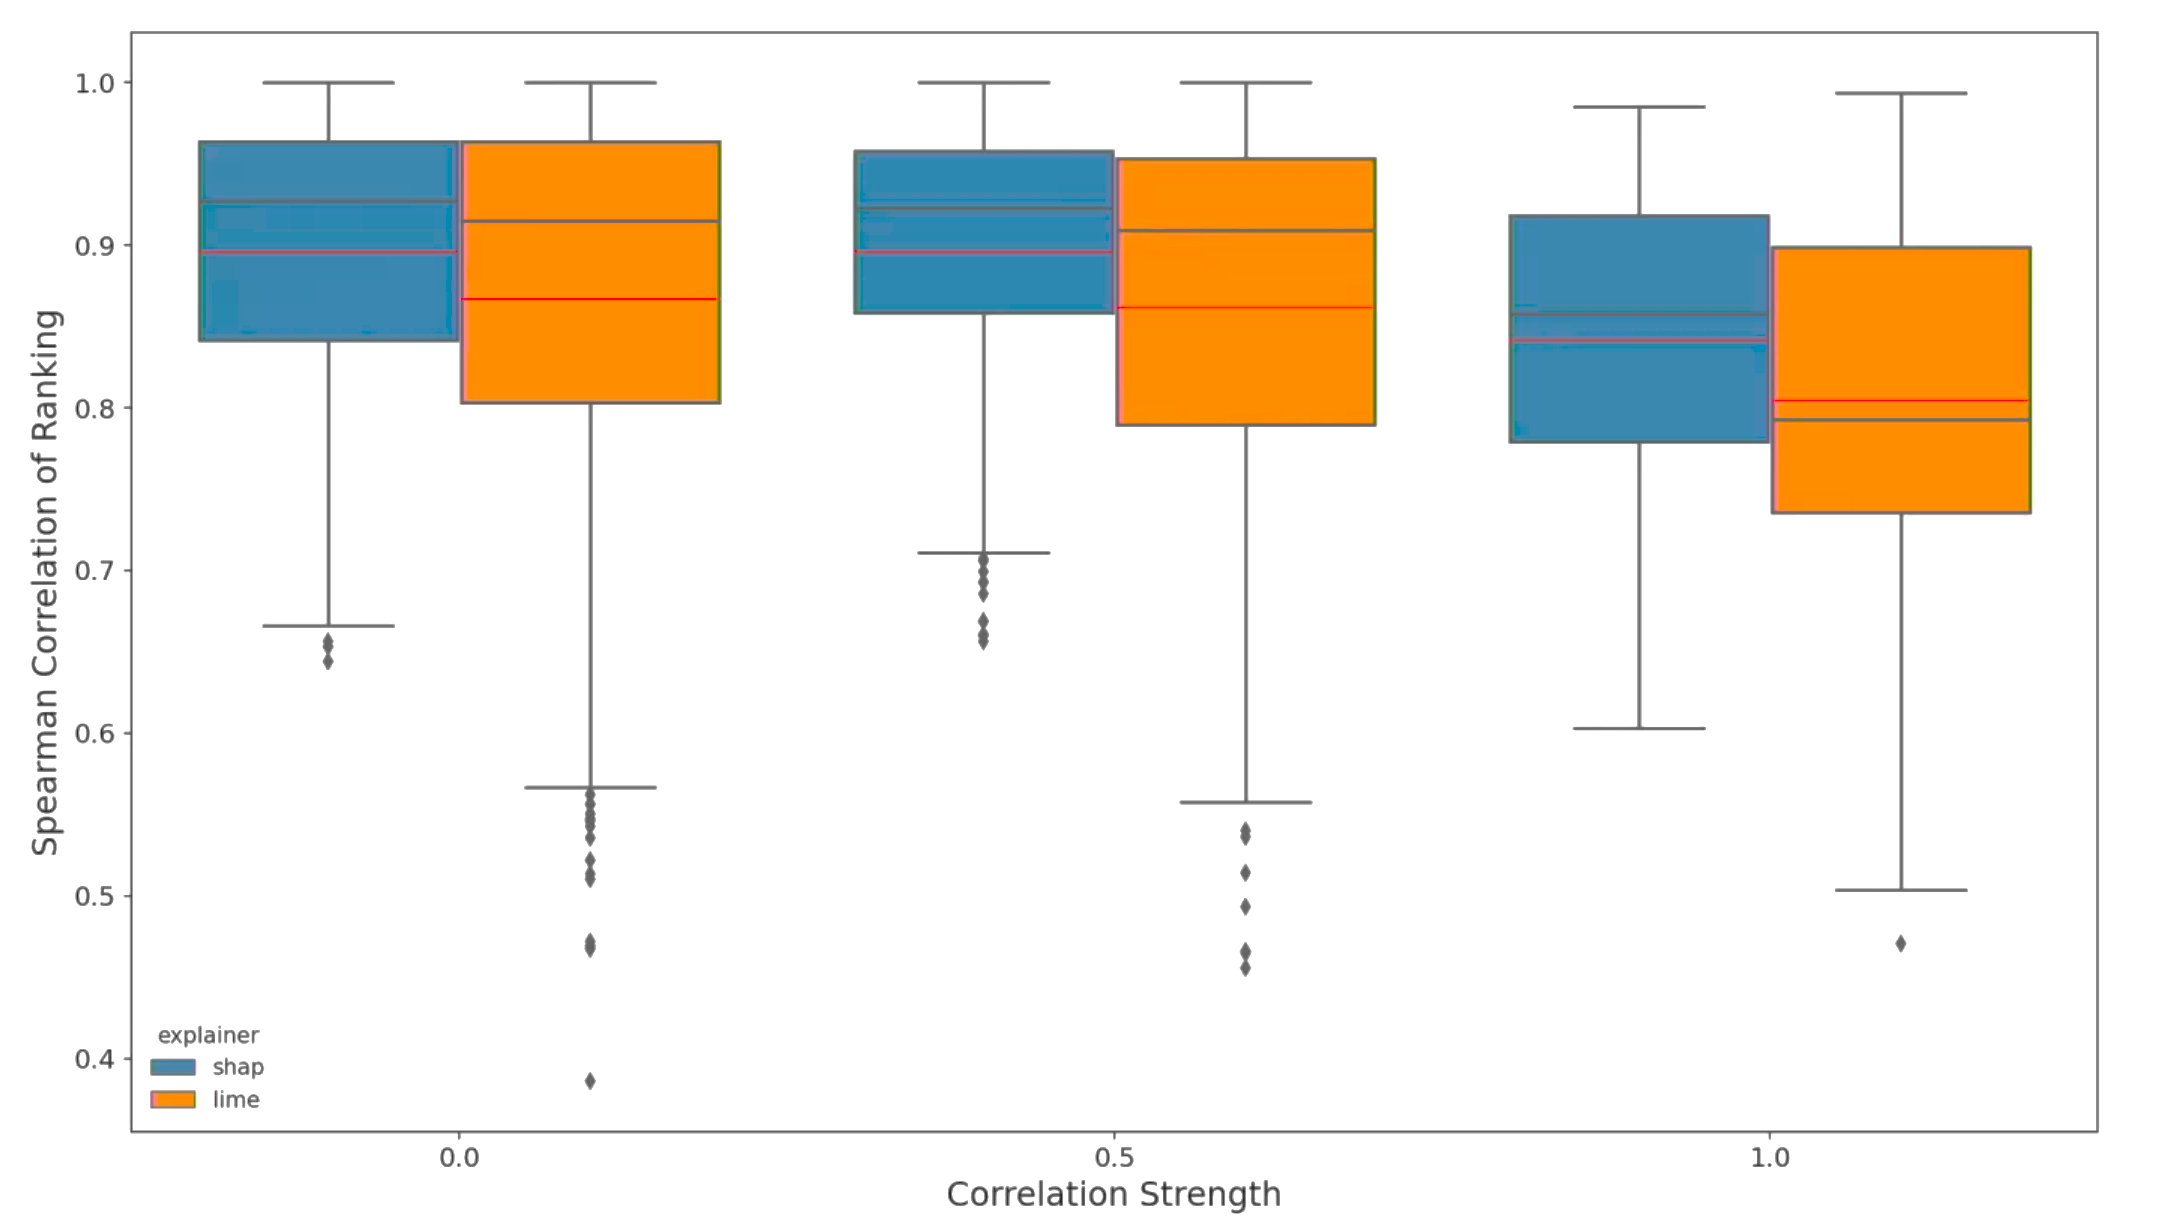
\includegraphics[width=0.45\textwidth]{media/image17.png}
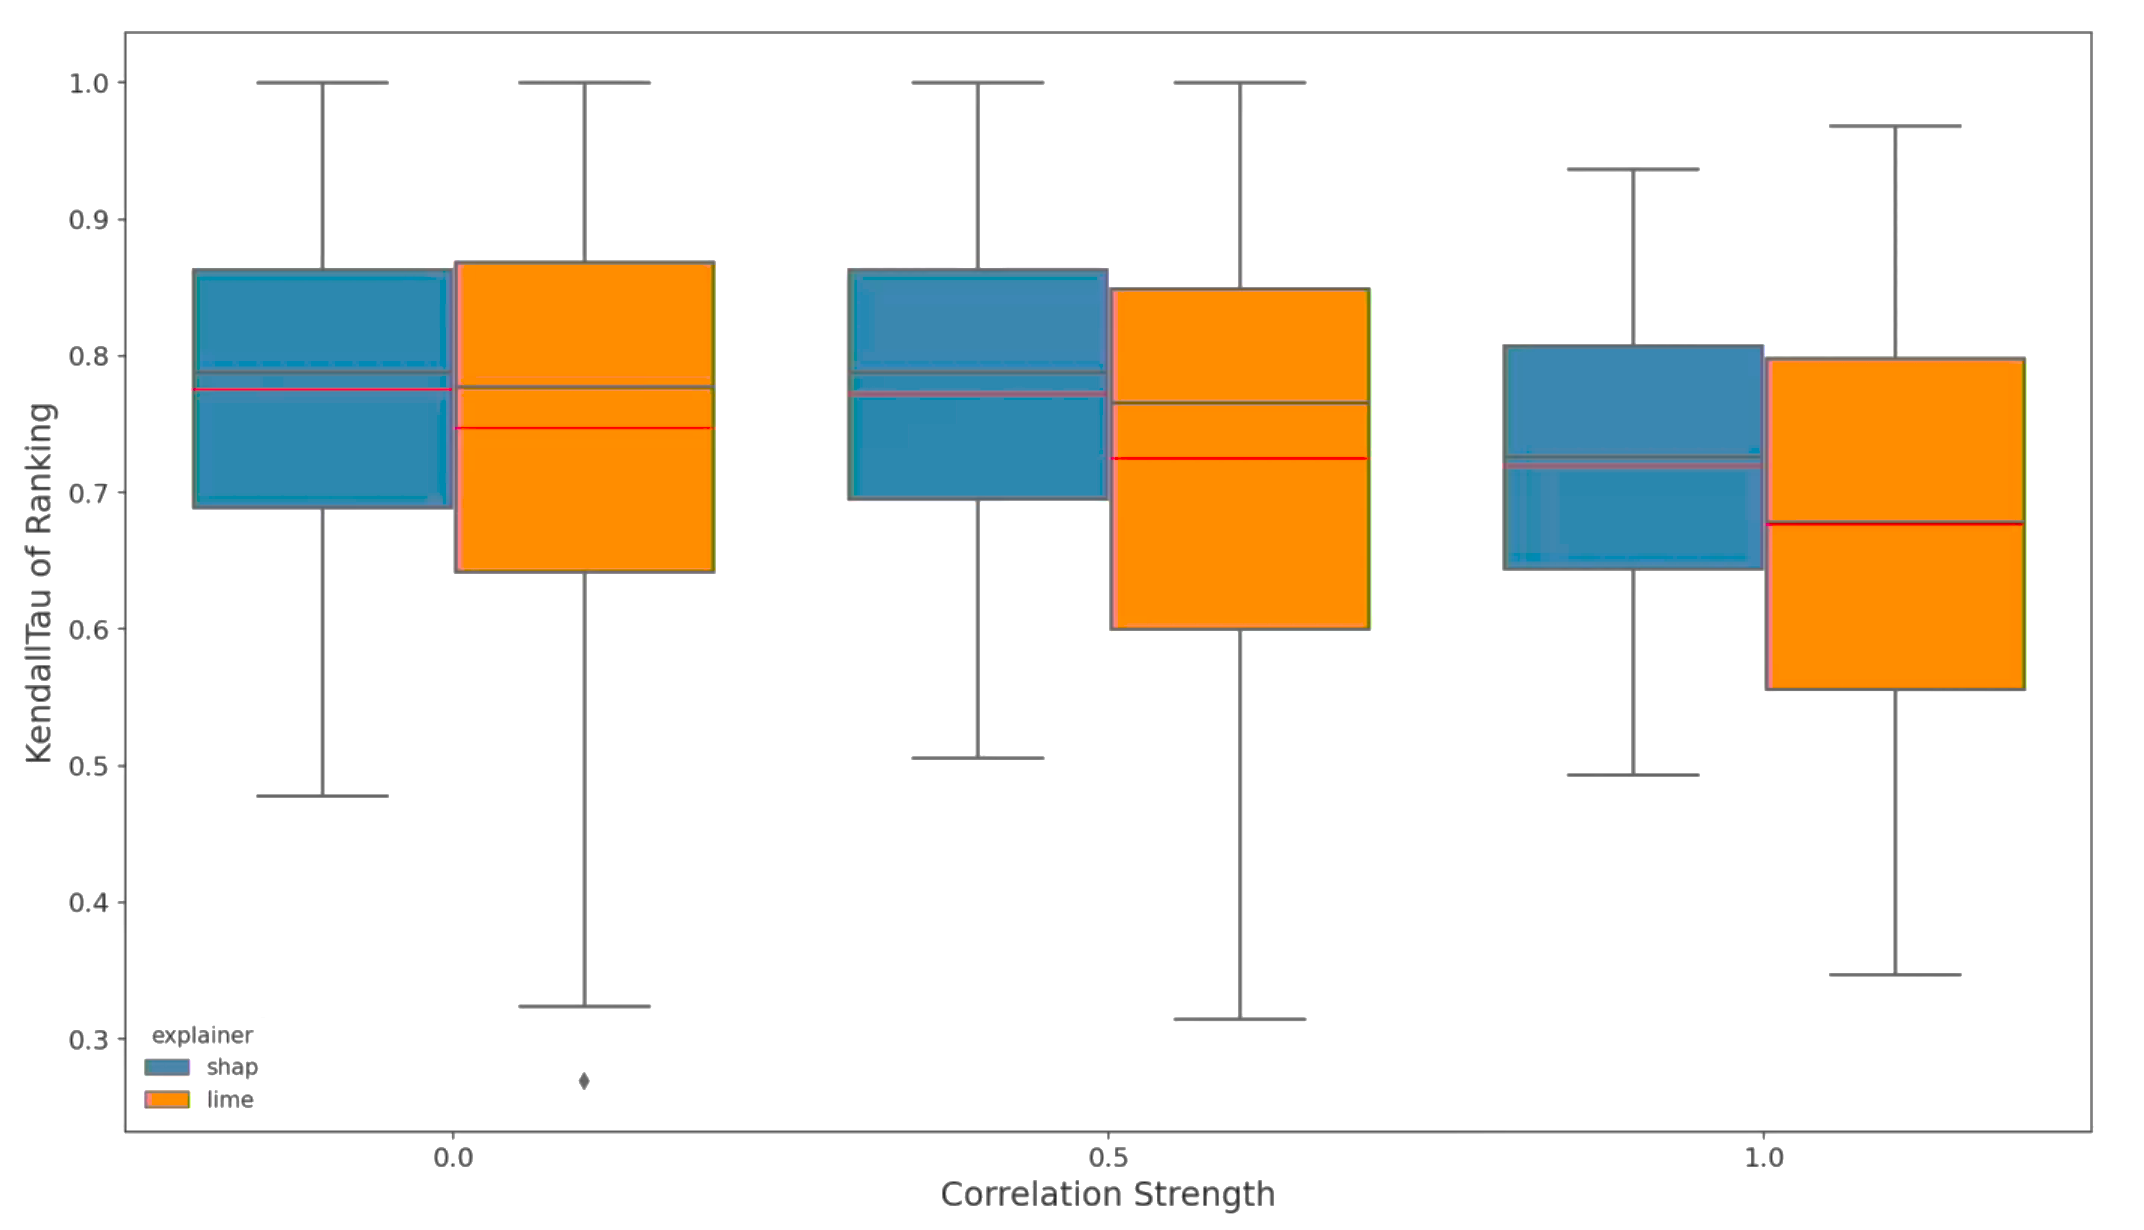
\includegraphics[width=0.45\textwidth]{media/image18.png}
\caption{Fig 10.1 Local Spearman Correlation of Explanations (LIME/SHAP) Ranking Between M and G Under Different Correlation Strength (left) and Fig 10.2. Local Kendall Tau of Explanations (LIME/SHAP) Ranking Between M and G Under Different Correlation Strength (right)}
\end{figure}

\begin{figure}[H]
\centering
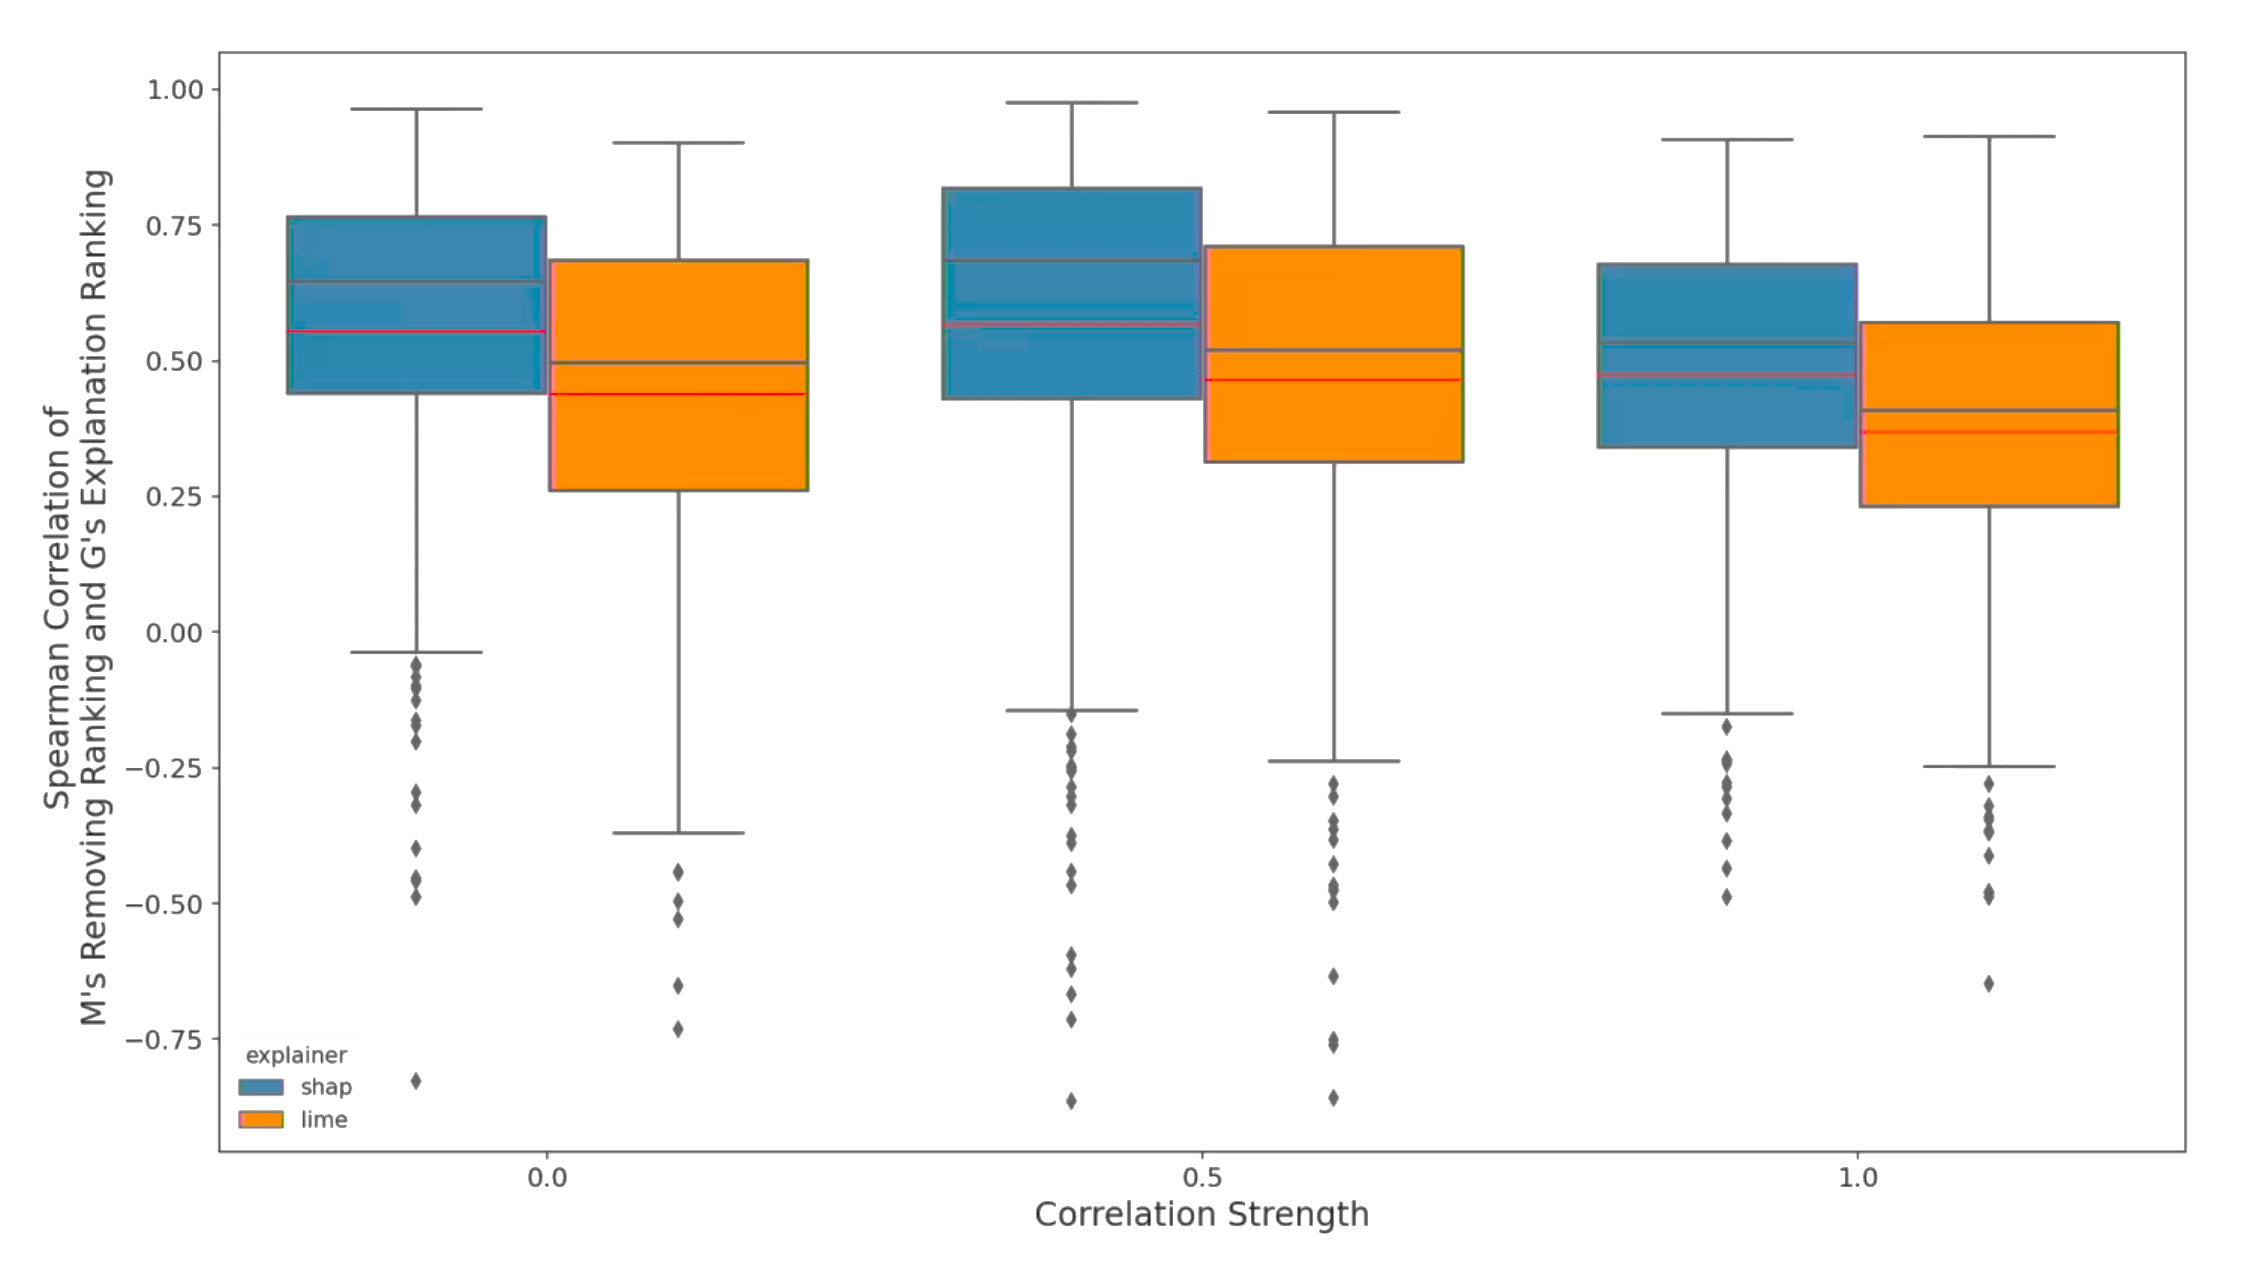
\includegraphics[width=0.45\textwidth]{media/image19.png}
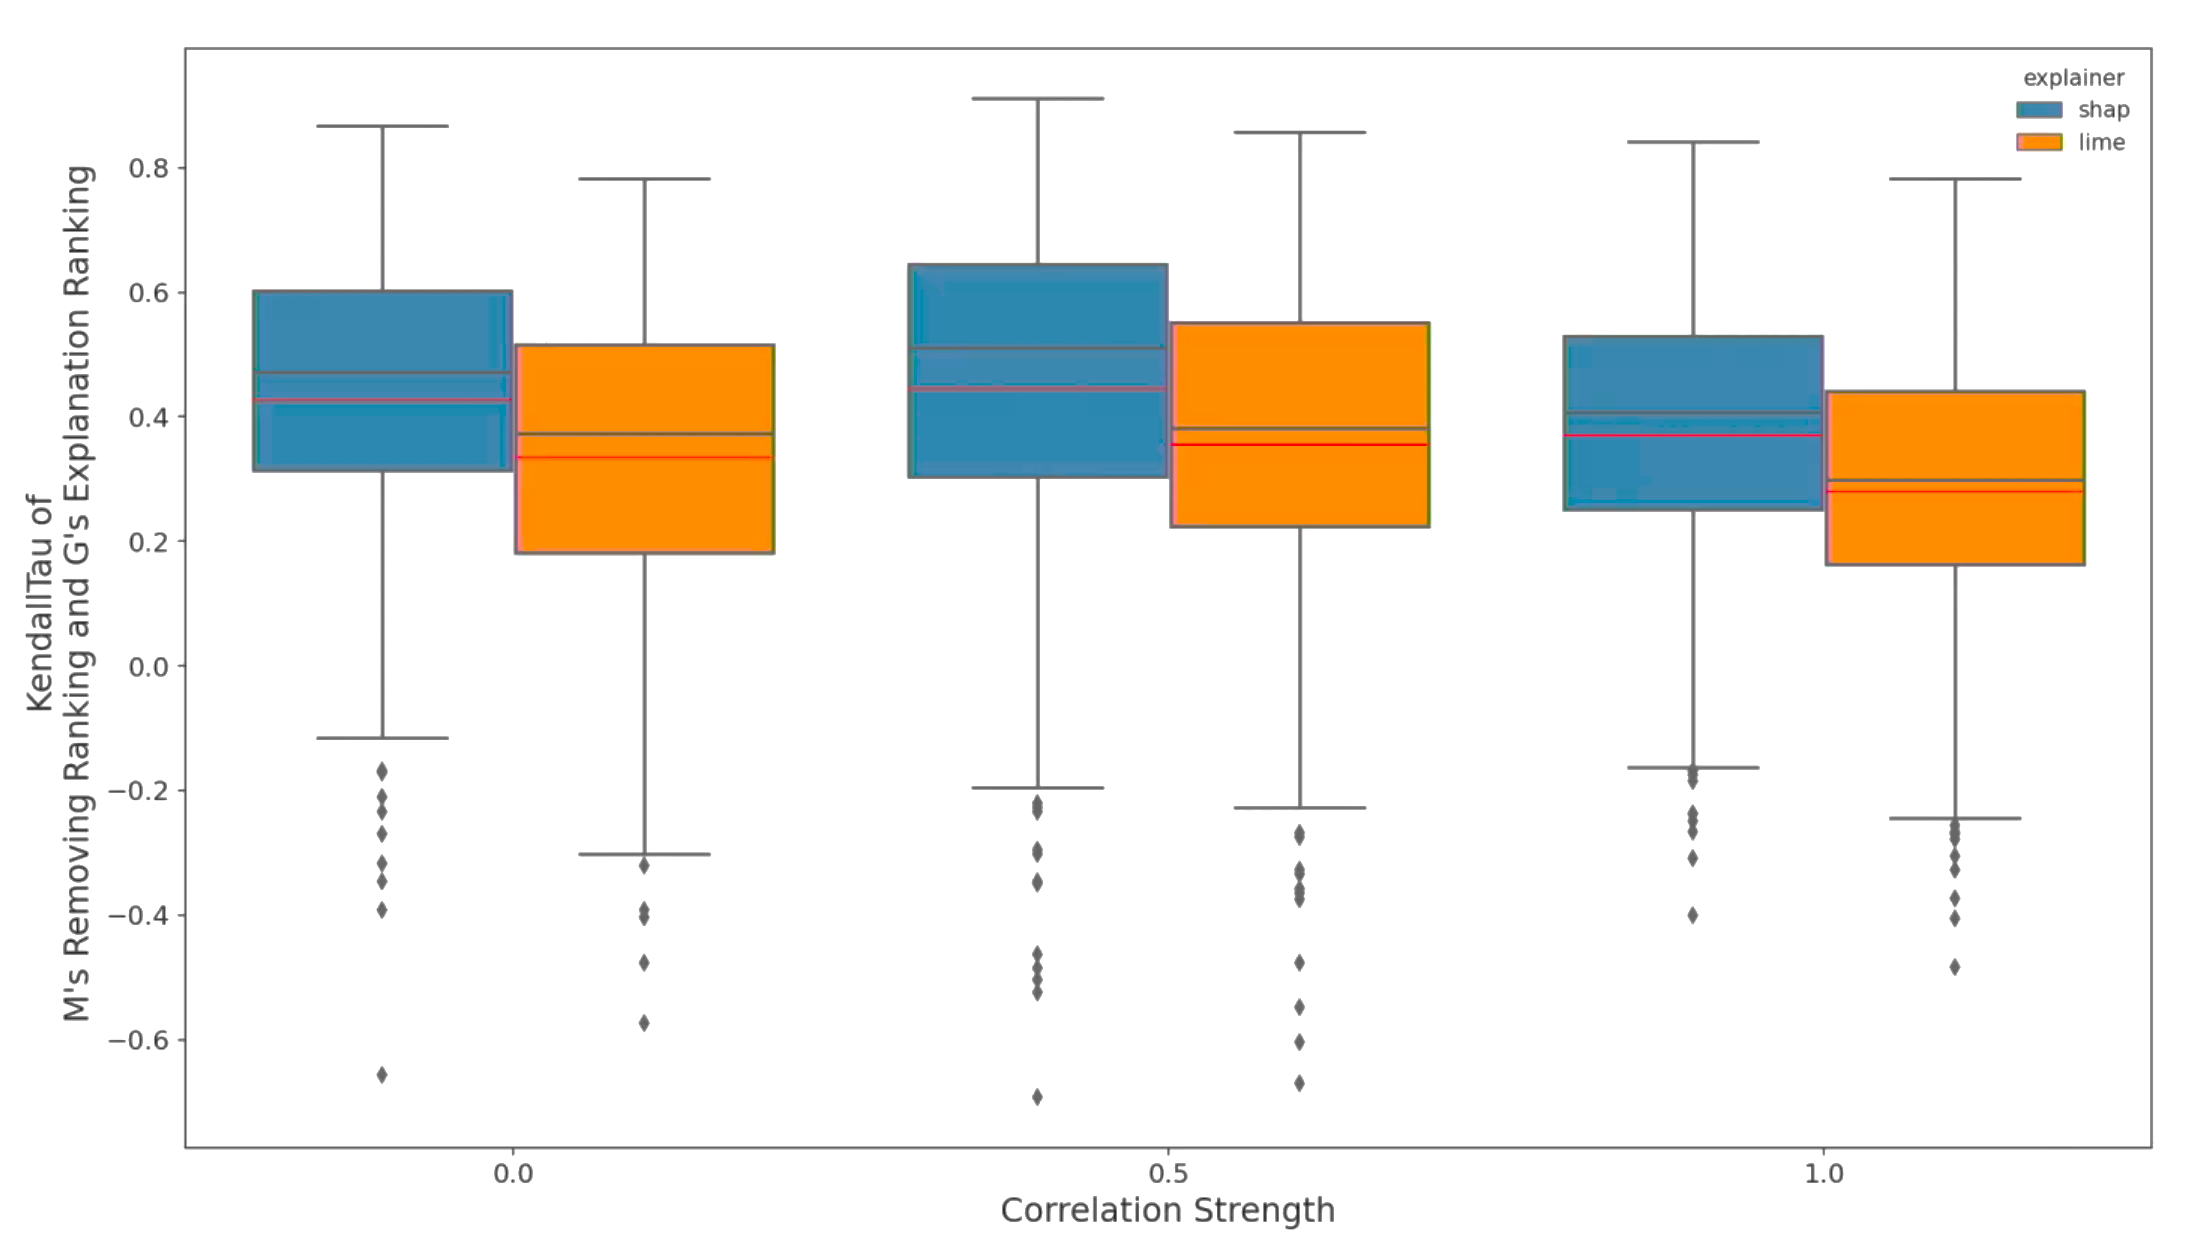
\includegraphics[width=0.45\textwidth]{media/image20.png}
\caption{Fig A.11.1 Remove Ranking Spearman Correlation of Explanations (LIME/SHAP) Ranking Between M and G Under Different Correlation Strength (left) and Fig A.11.2. Remove Ranking Kendall Tau of Explanations (LIME/SHAP) Ranking Between M and G Under Different Correlation Strength (right)}
\end{figure}

\begin{figure}[H]
\centering
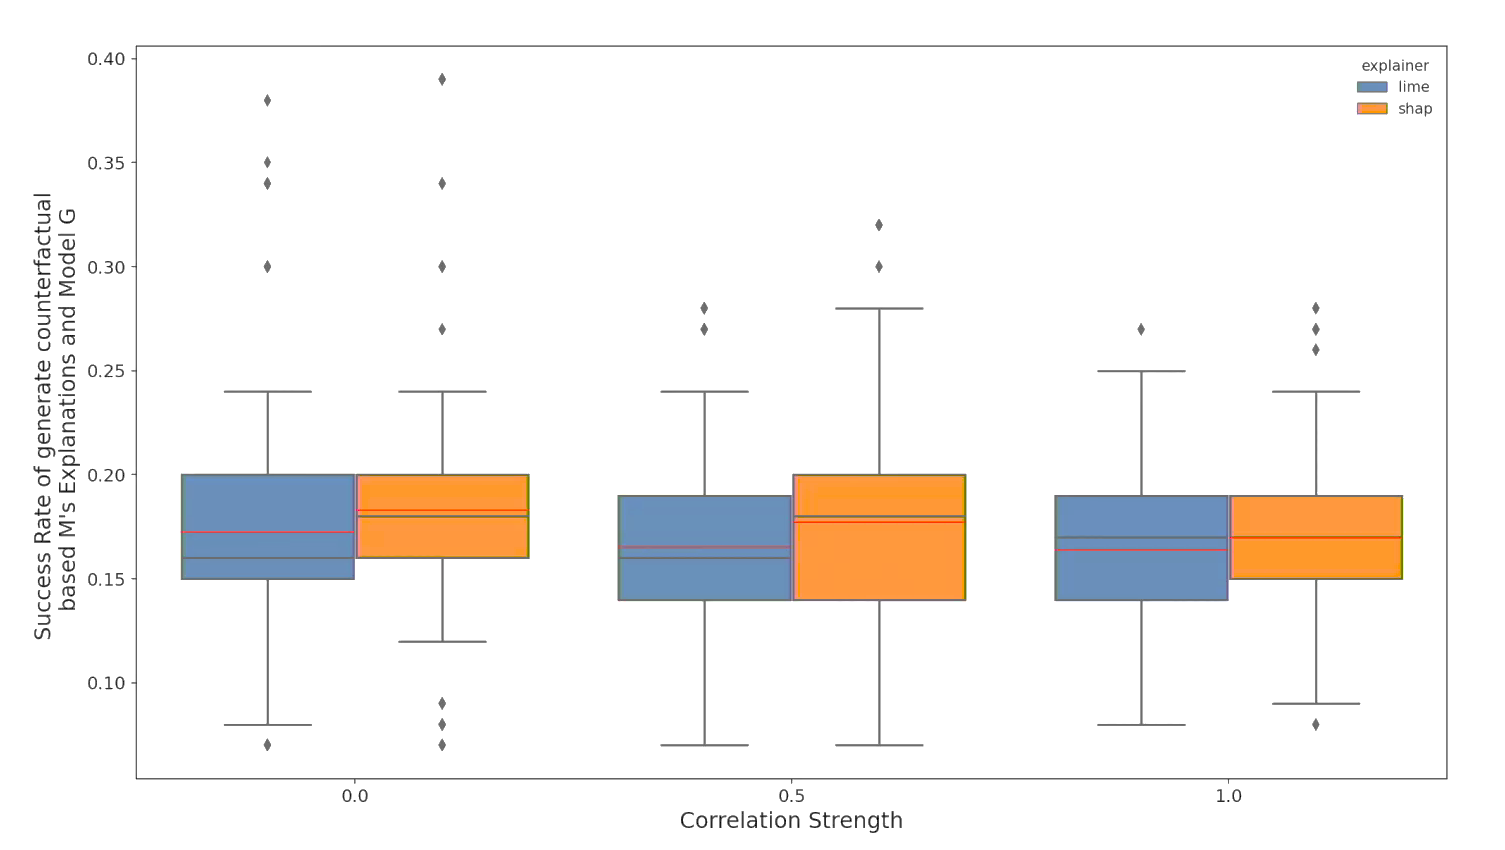
\includegraphics[width=0.7\textwidth]{media/image21.png}
\caption{Fig A.12.1 Success Rate of Generate Counterfactual based M's Explanations (LIME/SHAP) and Model G Under Different Correlation Strength}
\end{figure}

\begin{figure}[H]
\centering
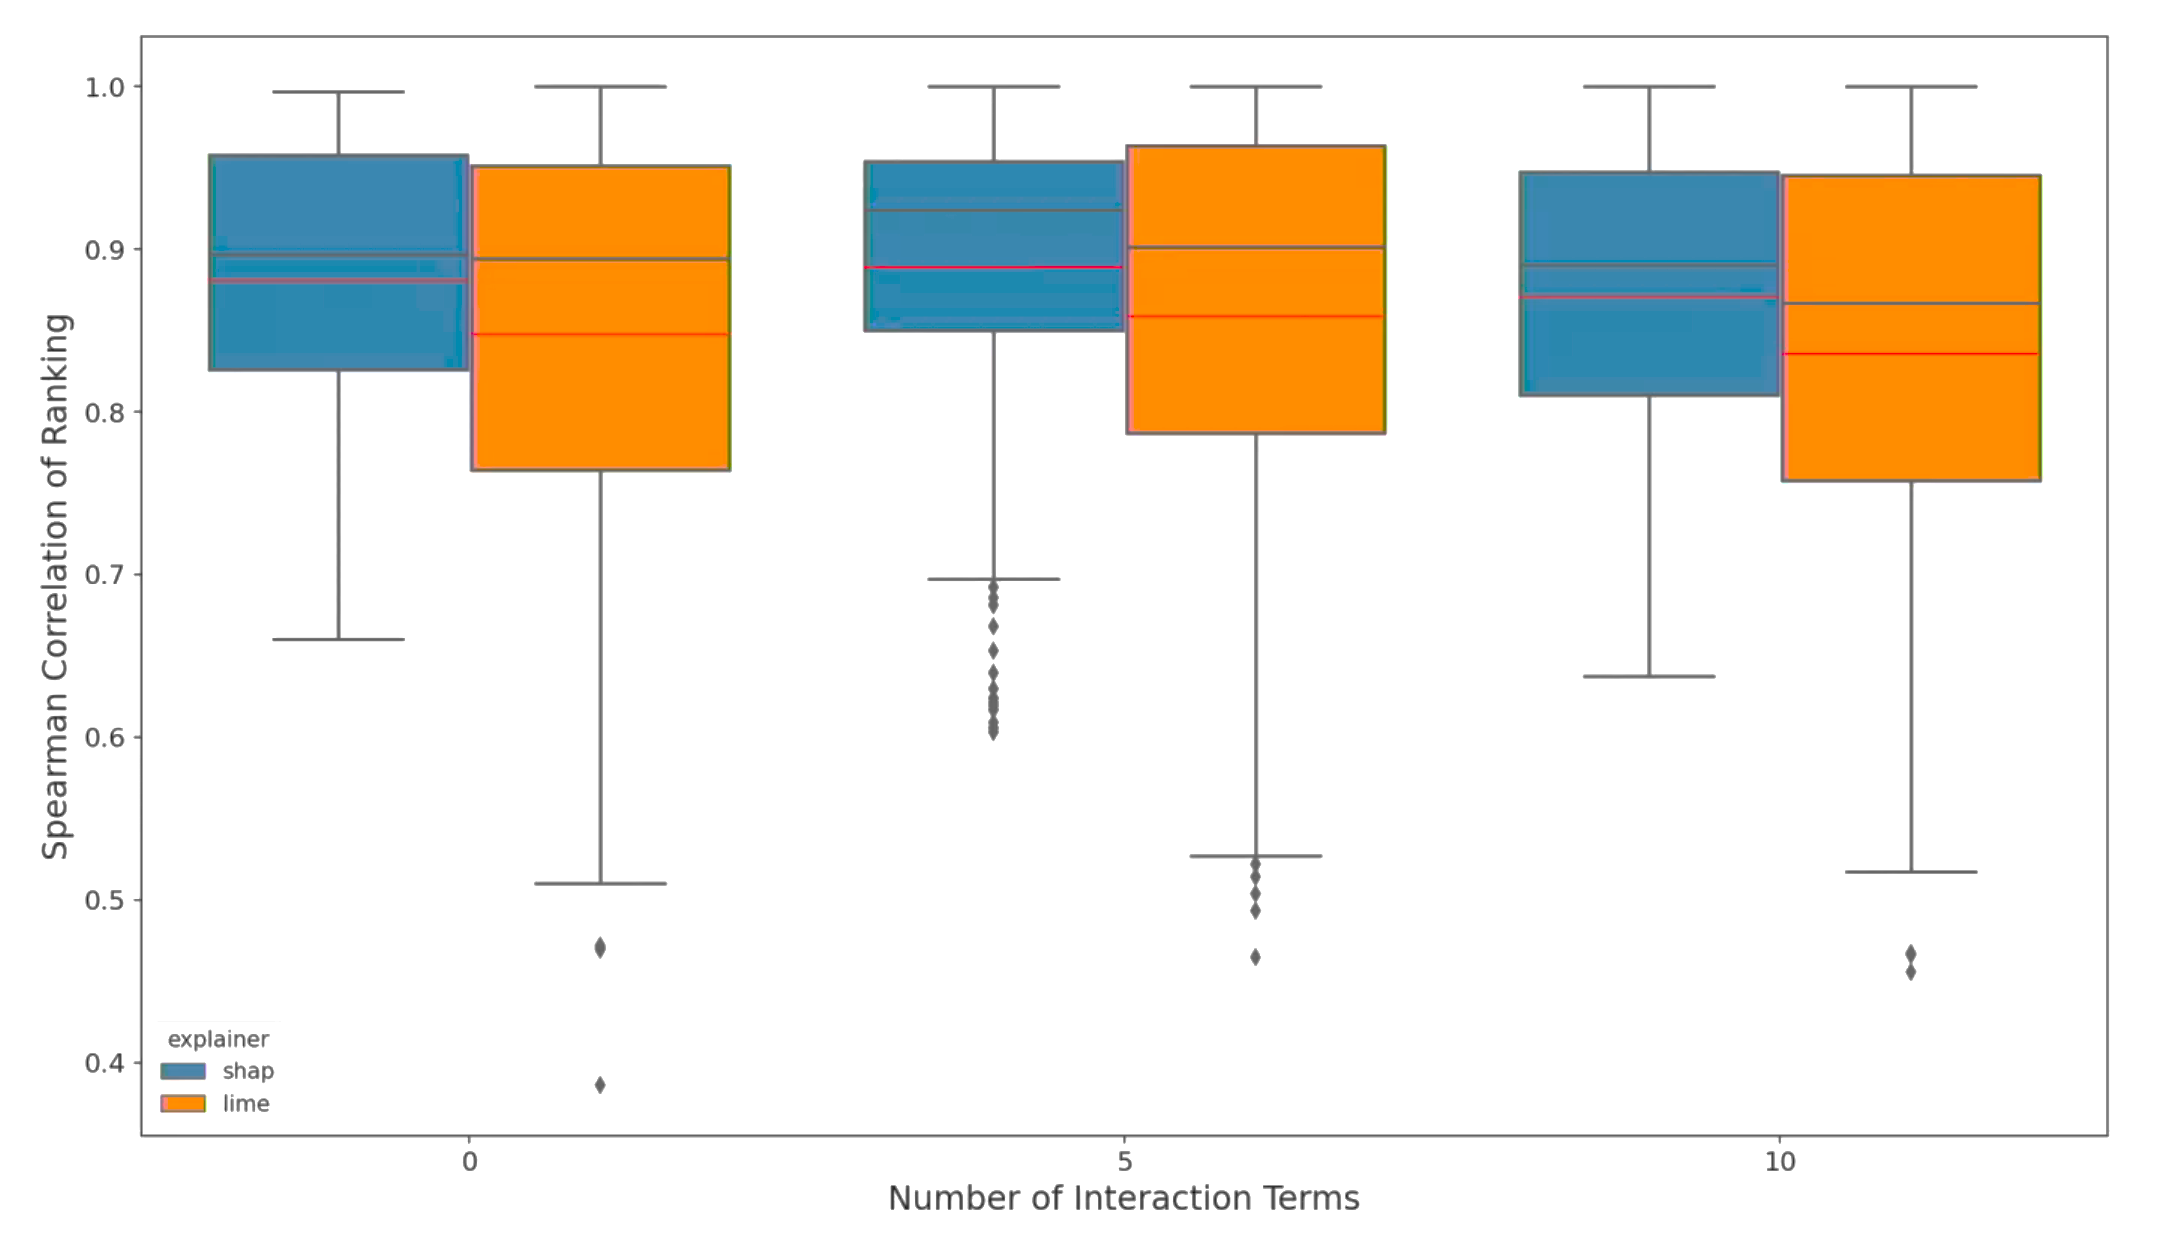
\includegraphics[width=0.45\textwidth]{media/image22.png}
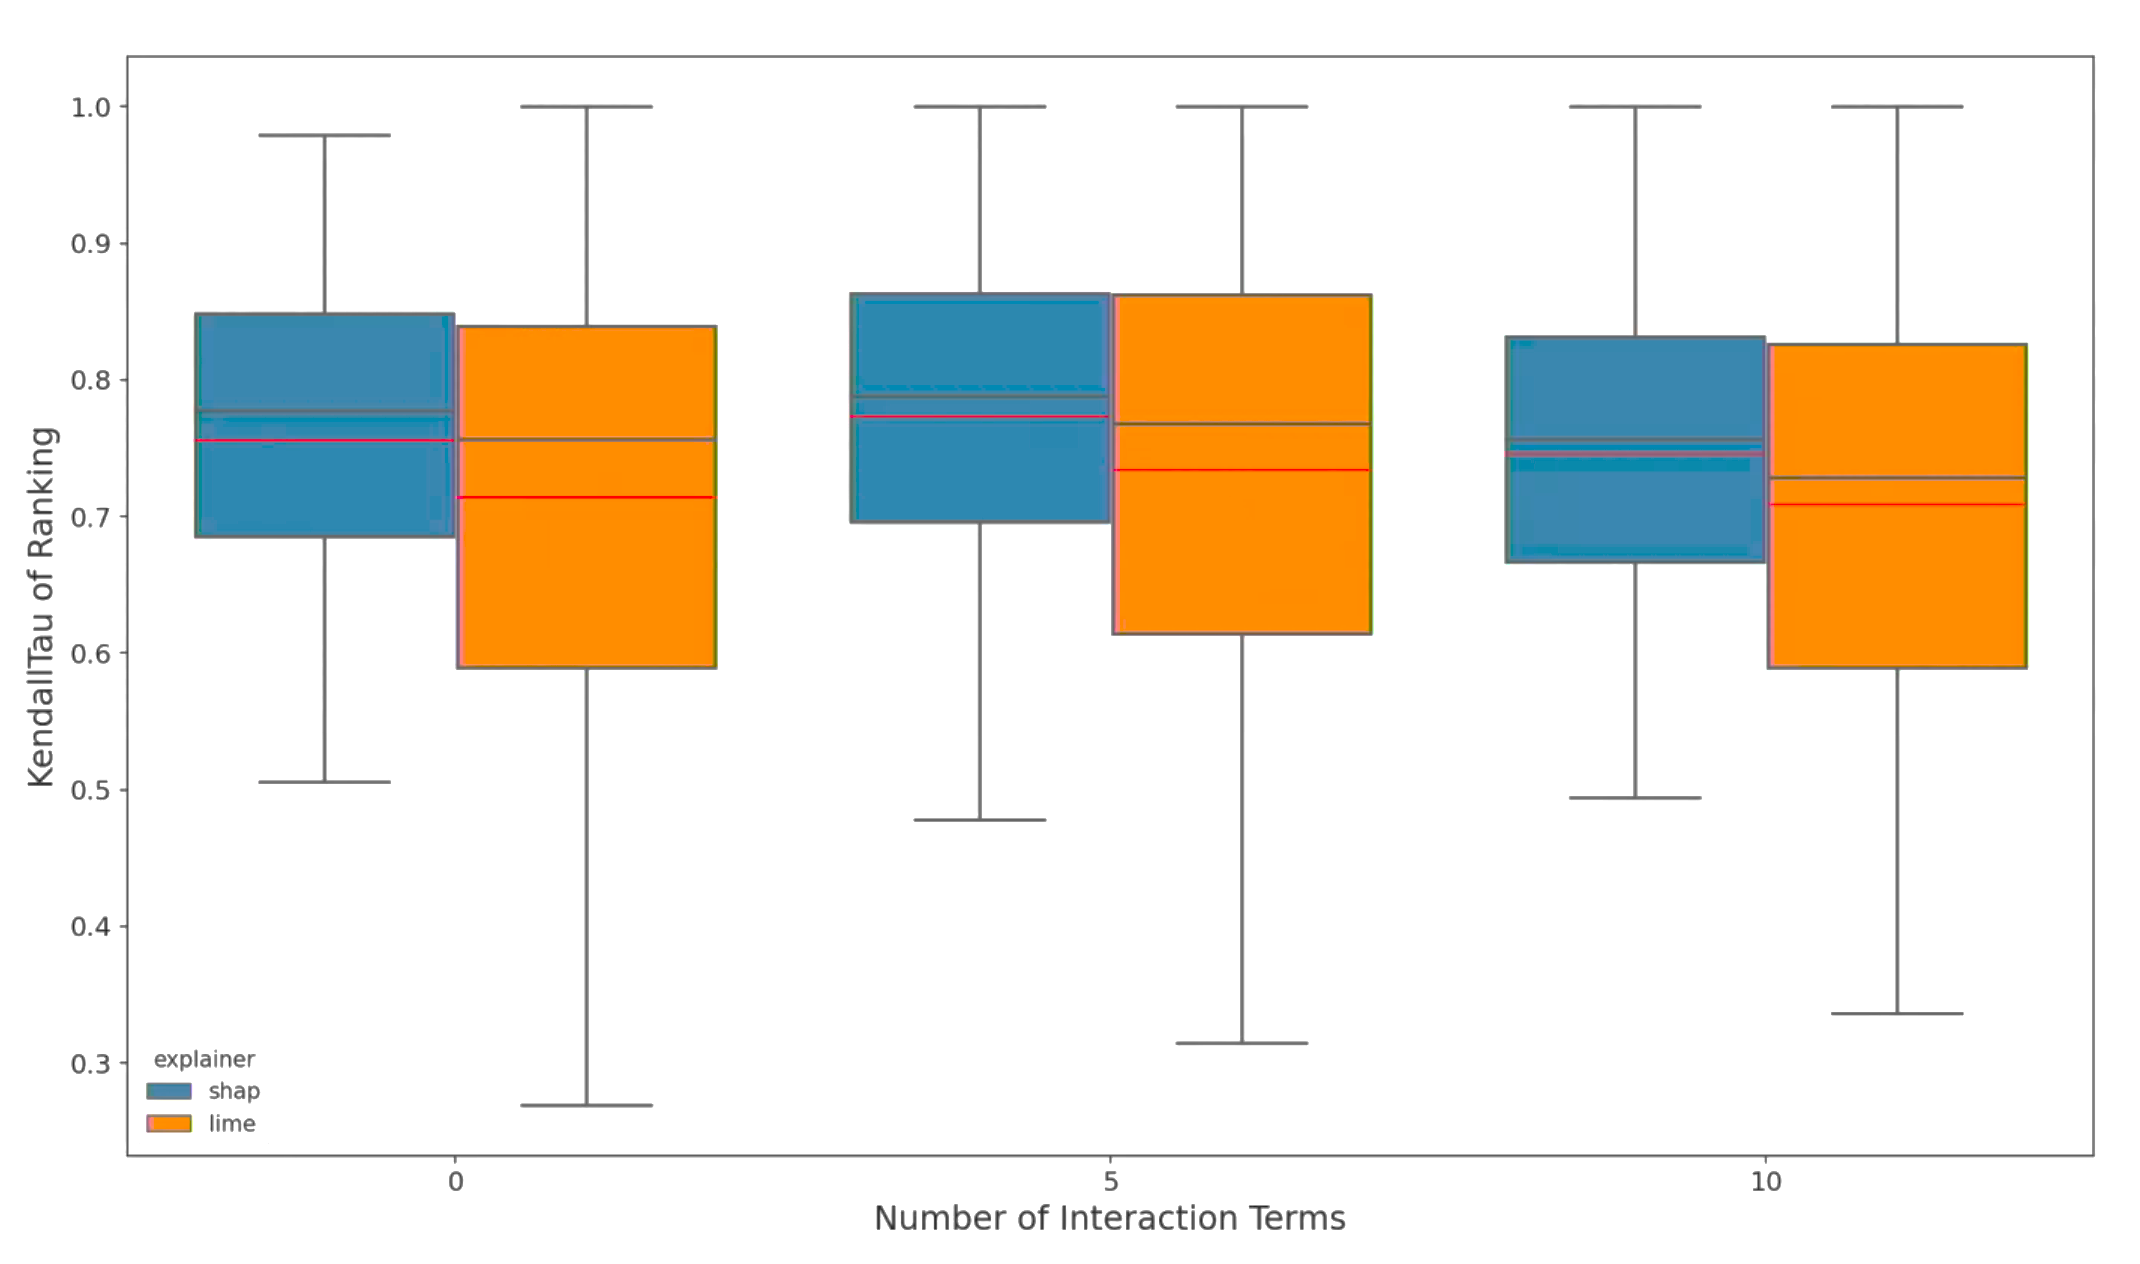
\includegraphics[width=0.45\textwidth]{media/image23.png}
\caption{Fig 13.1 Global Spearman Correlation of Explanations (LIME/SHAP) Ranking Between M and G Under Different Interaction Number (left) and Fig 13.2. Global Kendall Tau of Explanations (LIME/SHAP) Ranking Between M and G Under Different Interaction Number (right)}
\end{figure}

\begin{figure}[H]
\centering
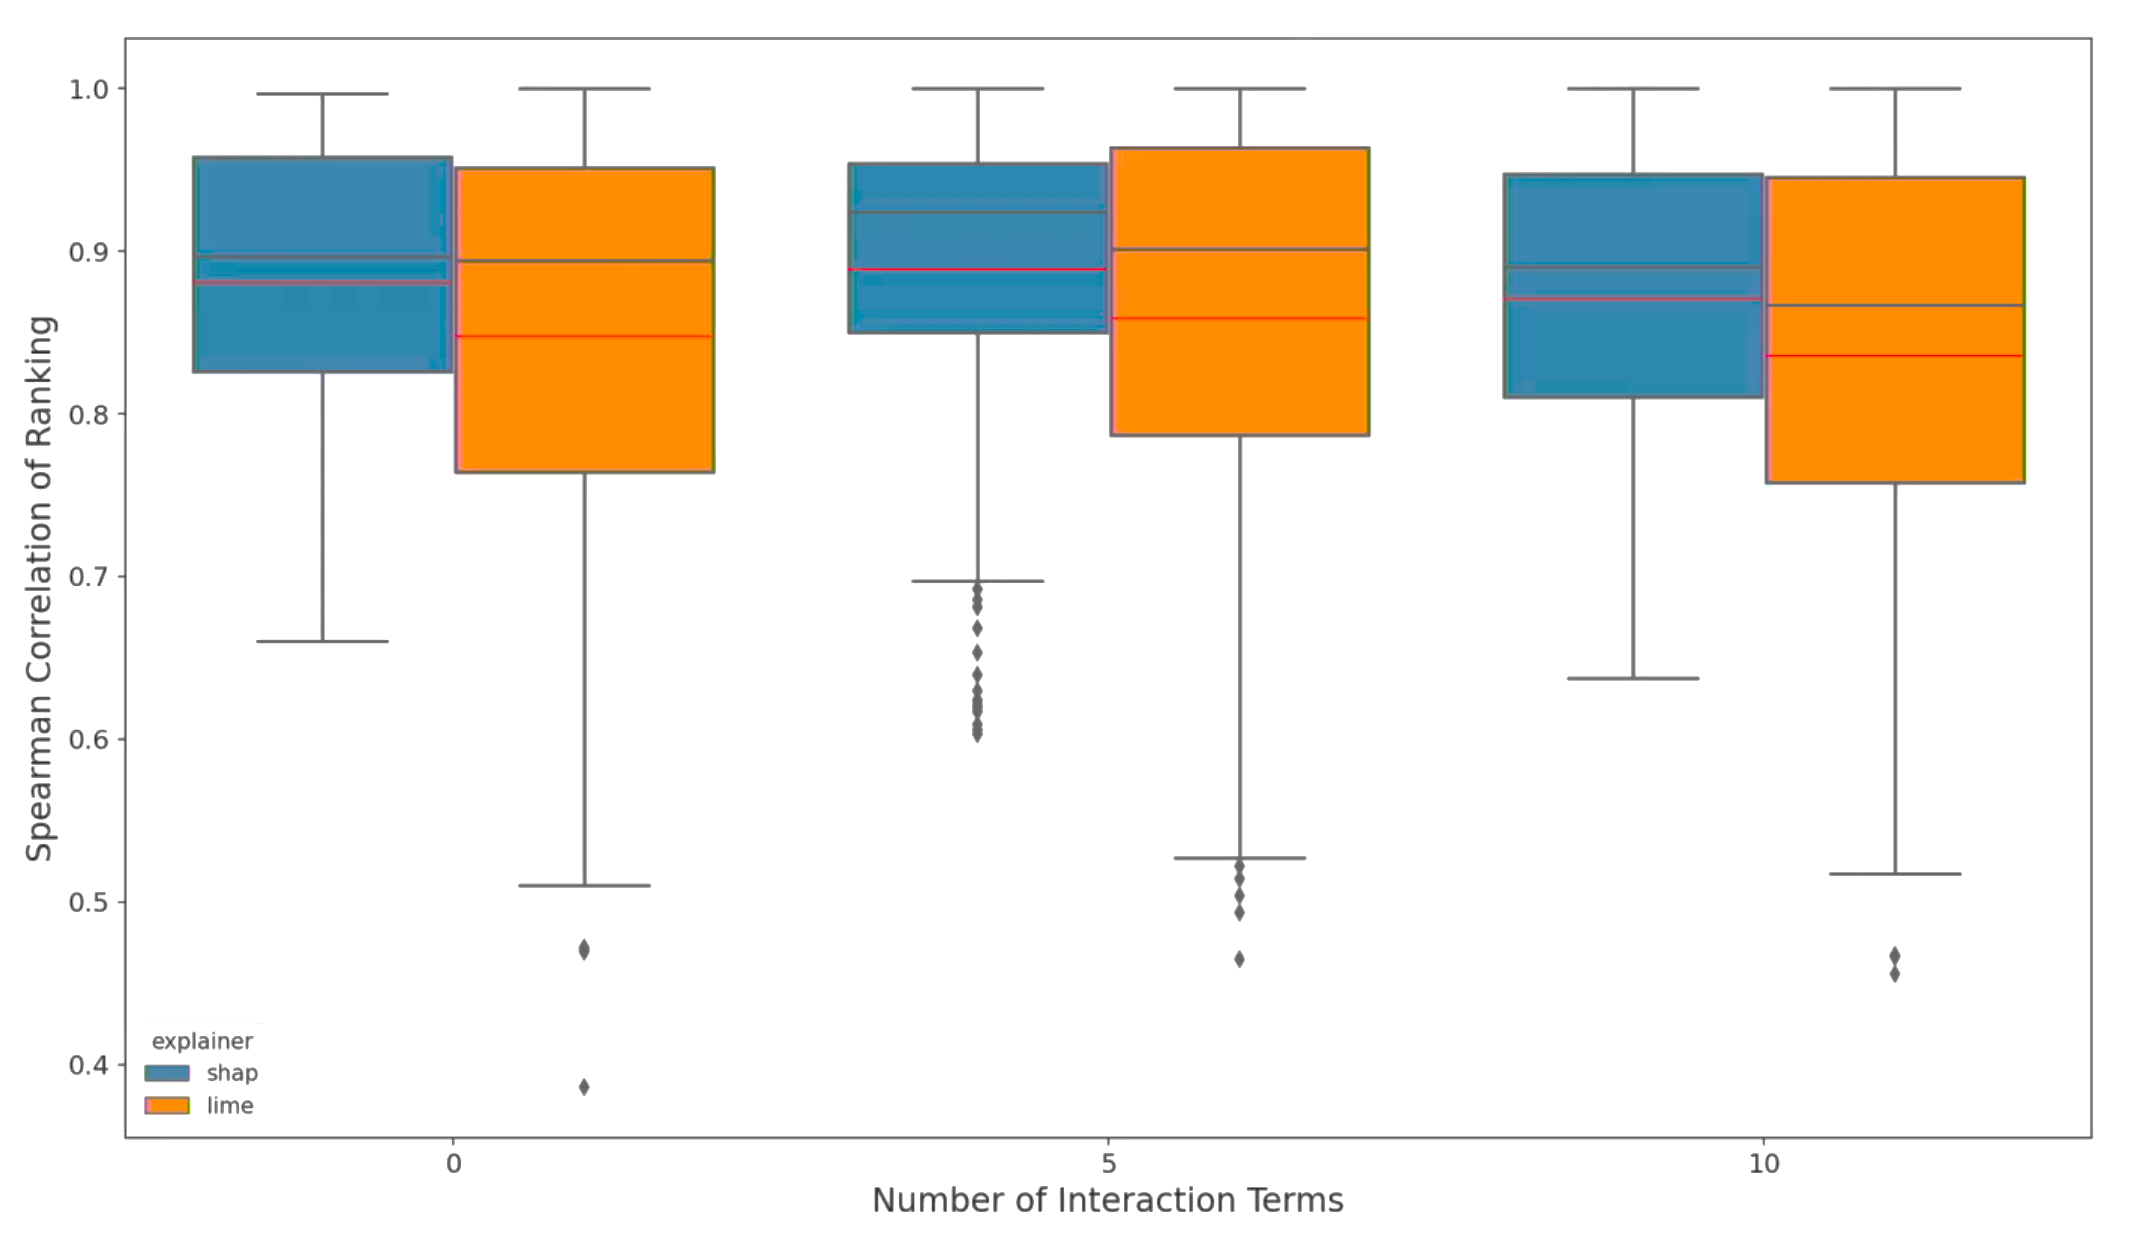
\includegraphics[width=0.45\textwidth]{media/image24.png}
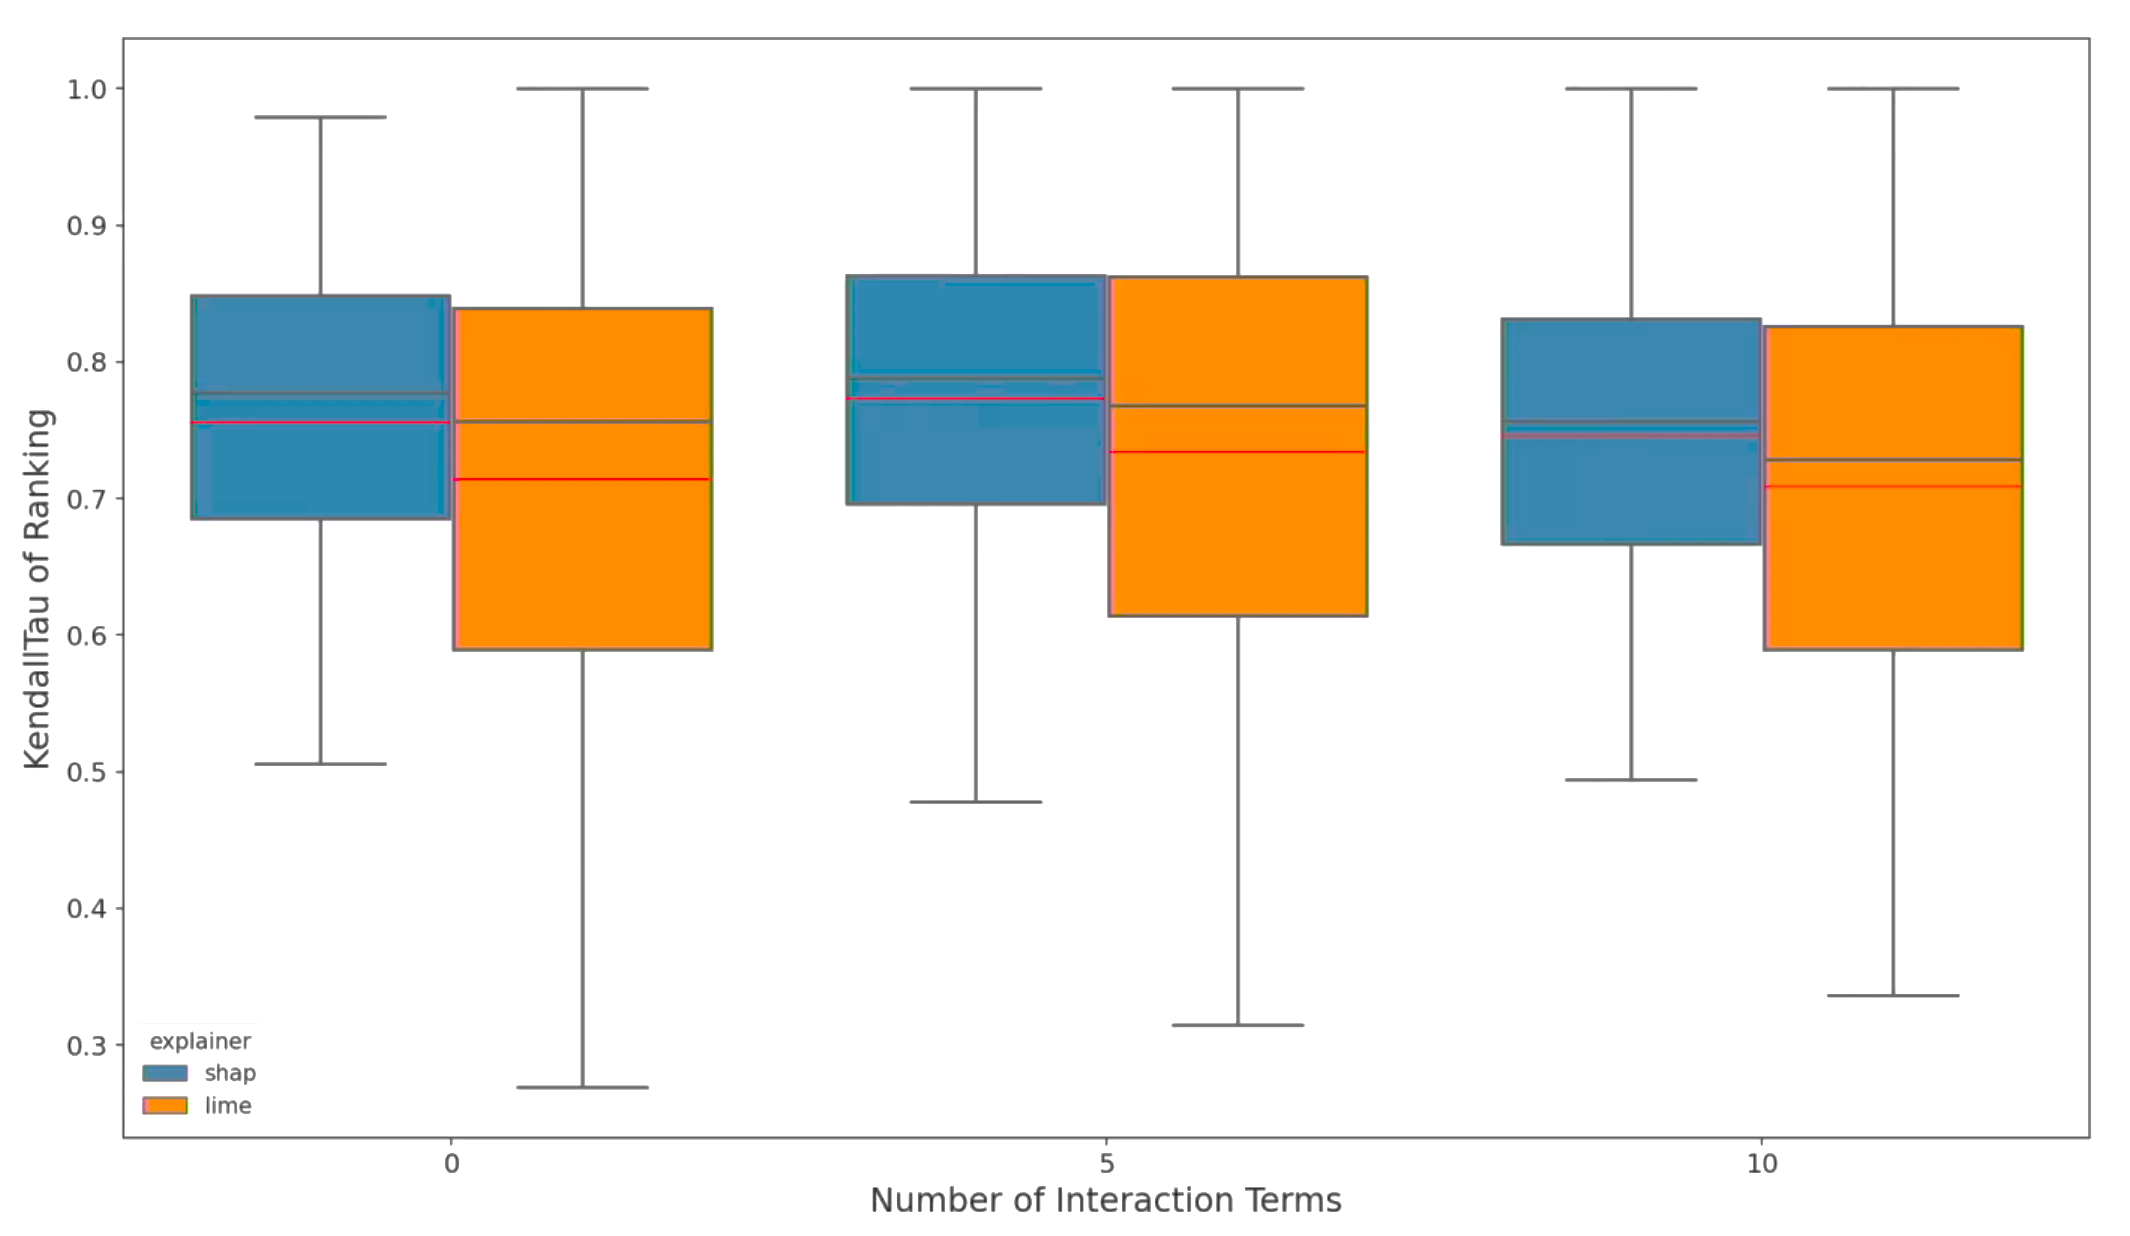
\includegraphics[width=0.45\textwidth]{media/image25.png}
\caption{Fig 14.1 Local Spearman Correlation of Explanations (LIME/SHAP) Ranking Between M and G Under Different Interaction Number (left) and Fig 14.2. Local Kendall Tau of Explanations (LIME/SHAP) Ranking Between M and G Under Different Interaction Number (right)}
\end{figure}

\begin{figure}[H]
\centering
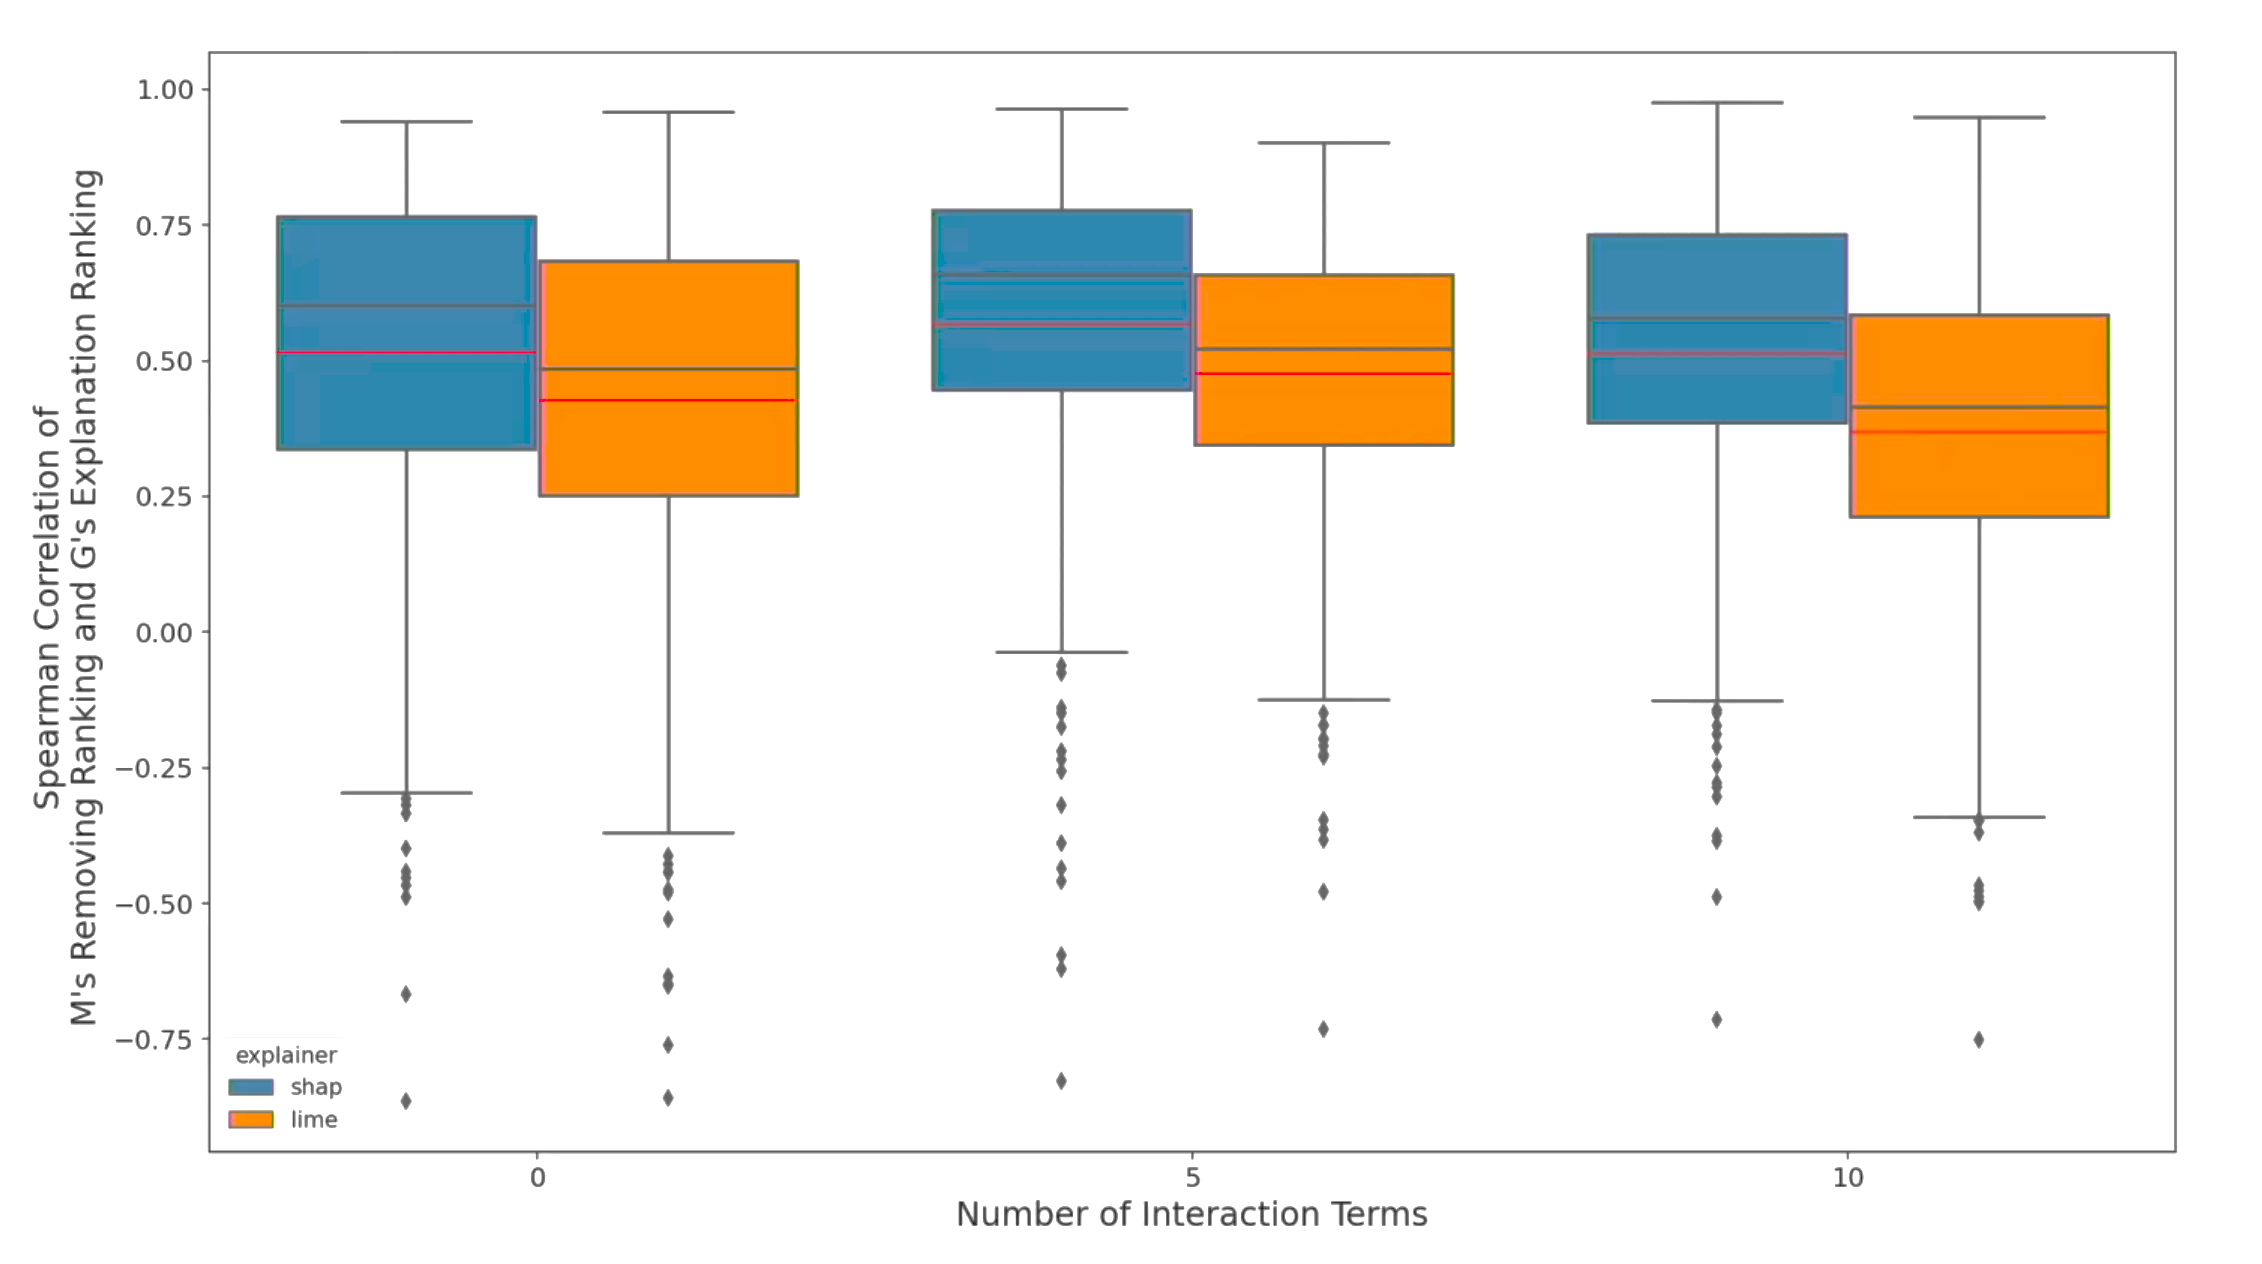
\includegraphics[width=0.45\textwidth]{media/image26.png}
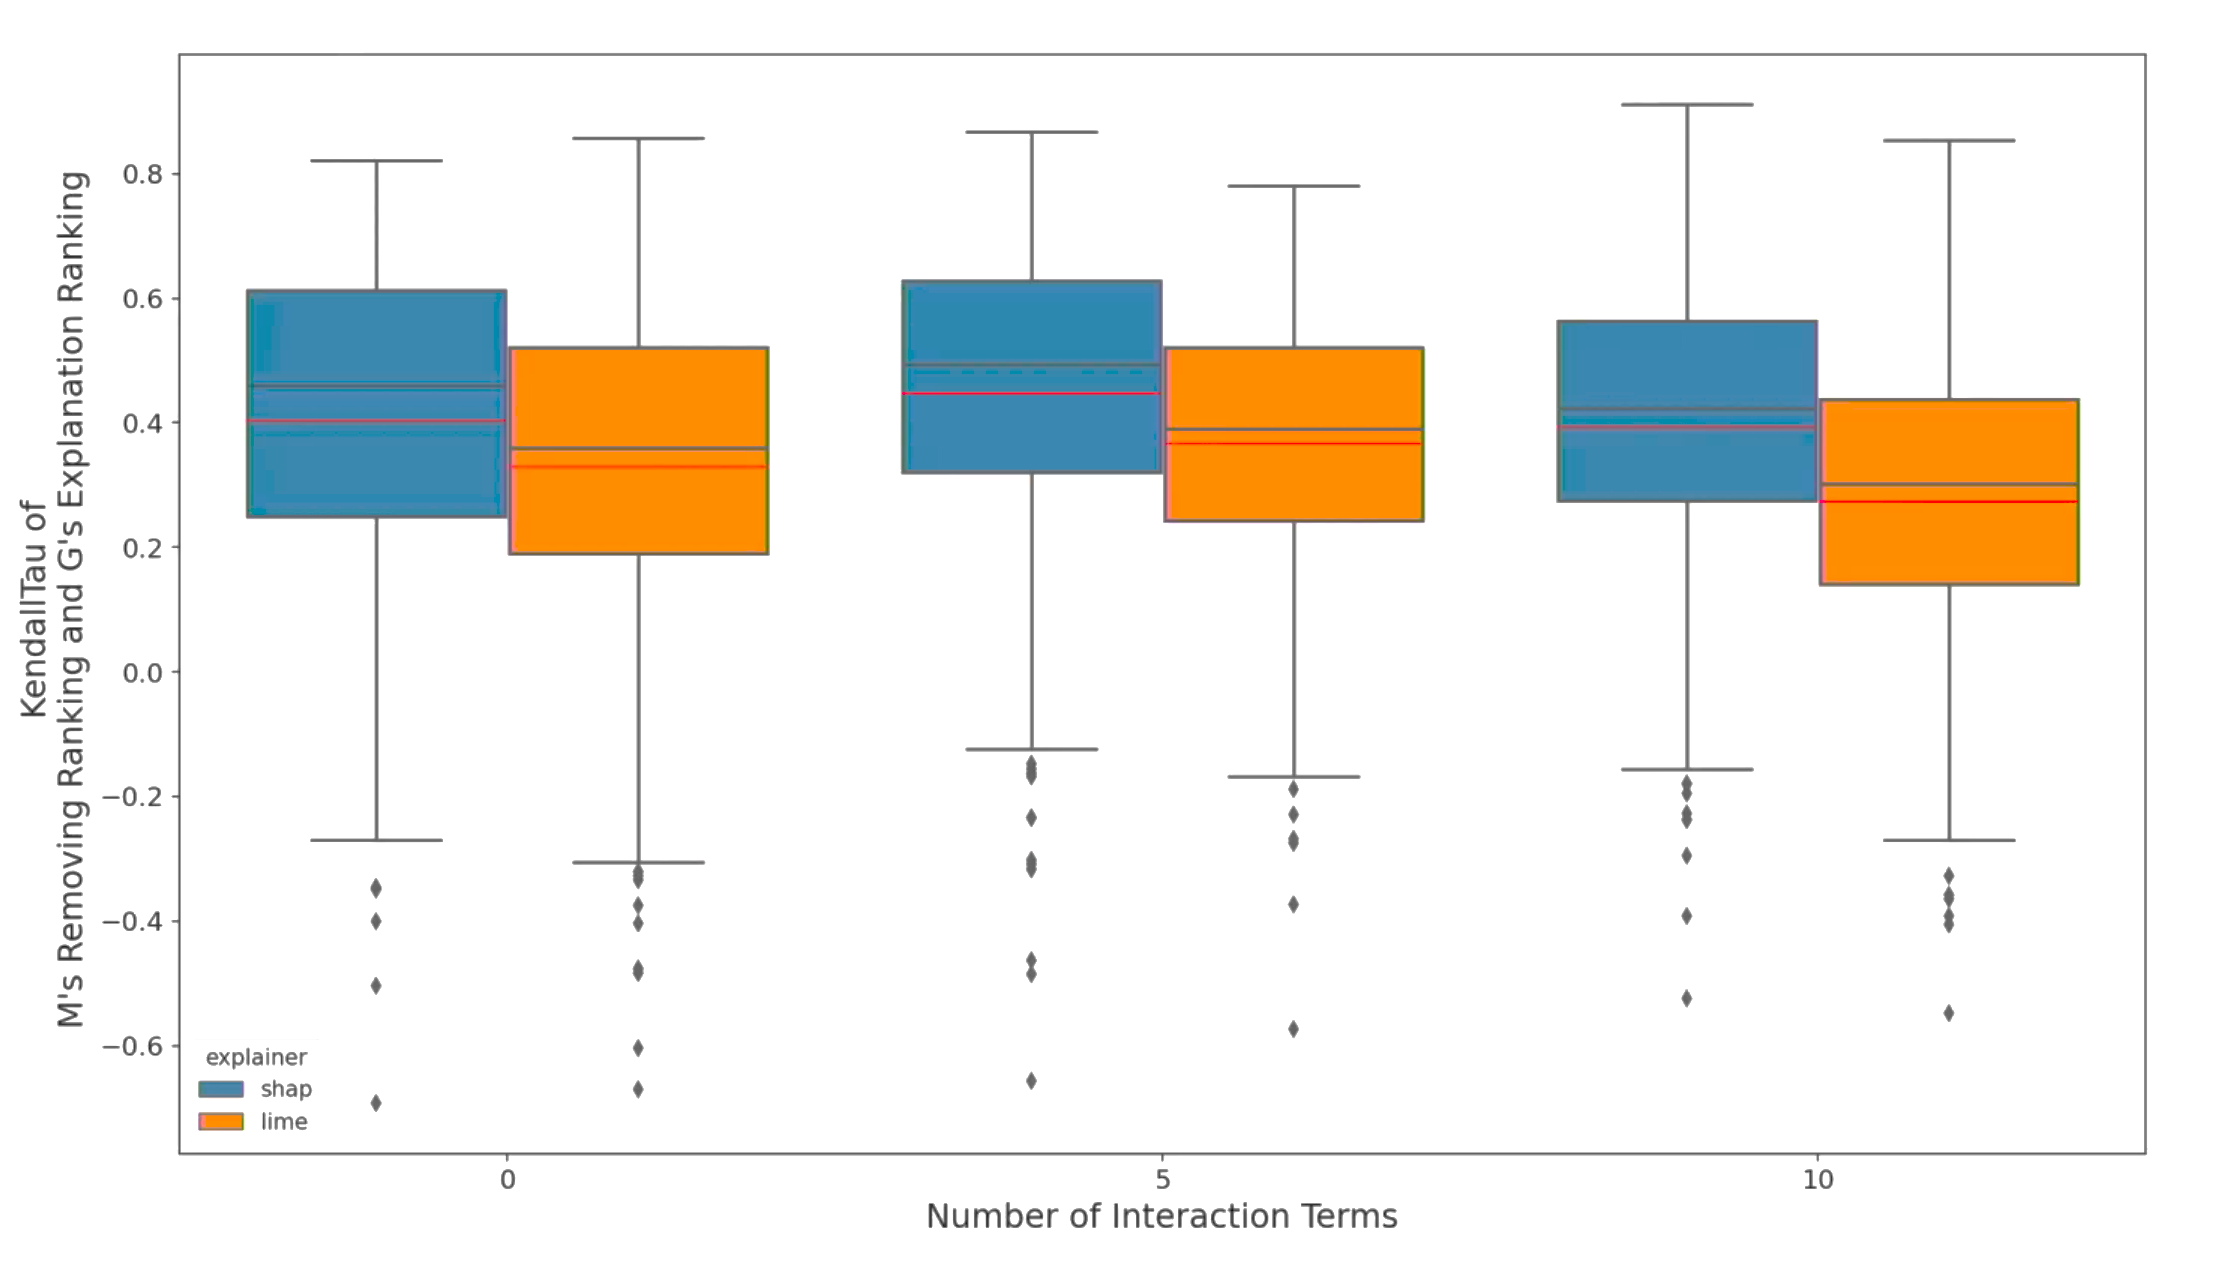
\includegraphics[width=0.45\textwidth]{media/image27.png}
\caption{Fig 15.1 Remove Ranking Spearman Correlation of Explanations (LIME/SHAP) Ranking Between M and G Under Different Interaction Number (left) and Fig 15.2. Remove Ranking Kendall Tau of Explanations (LIME/SHAP) Ranking Between M and G Under Different Interaction Number (right)}
\end{figure}

\begin{figure}[H]
\centering
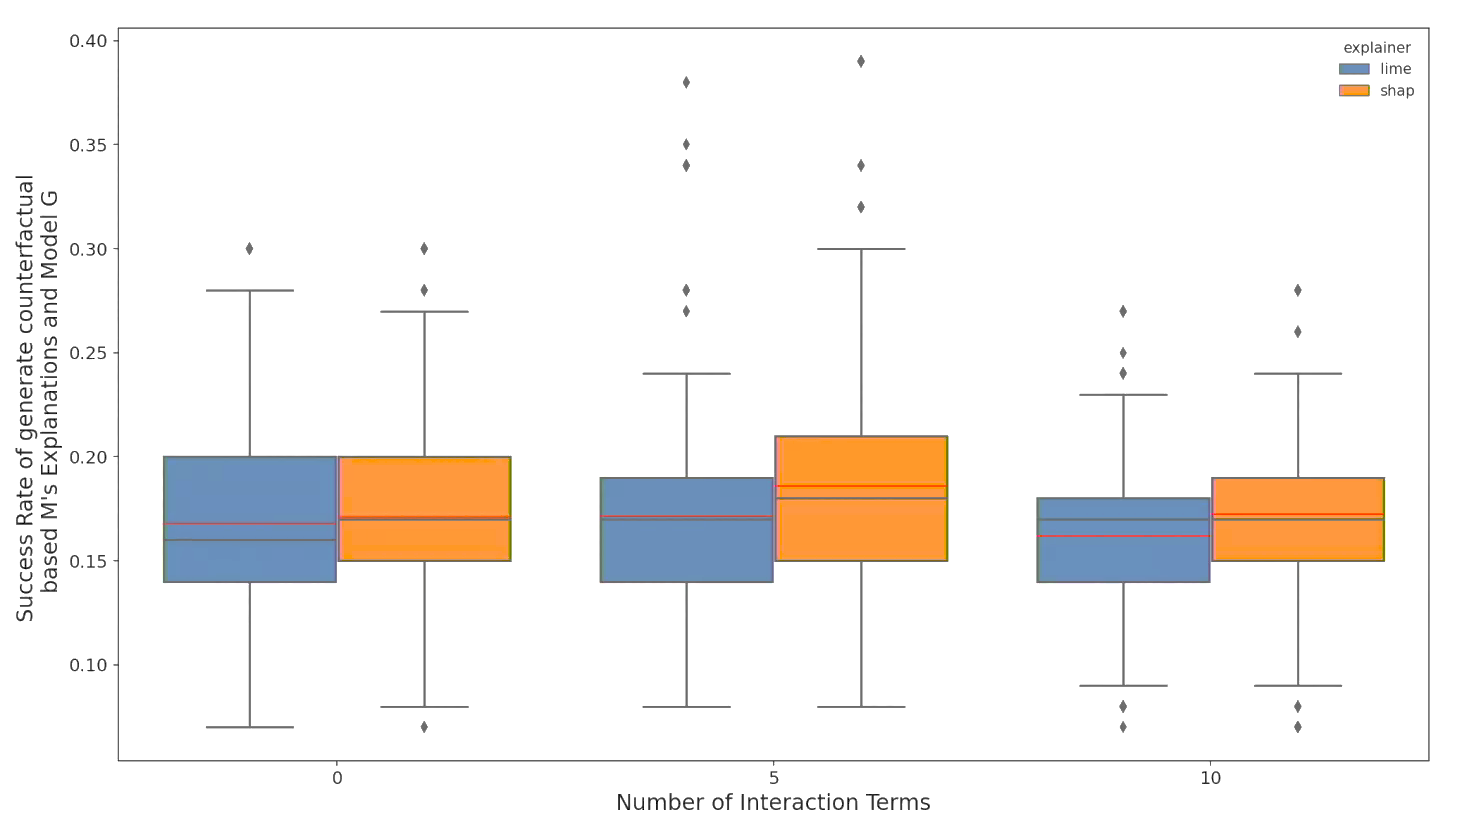
\includegraphics[width=0.7\textwidth]{media/image28.png}
\caption{Fig Success Rate of Generate Counterfactual based M's Explanations (LIME/SHAP) and Model G Under Different Interaction Number}
\end{figure}

\begin{figure}[H]
\centering
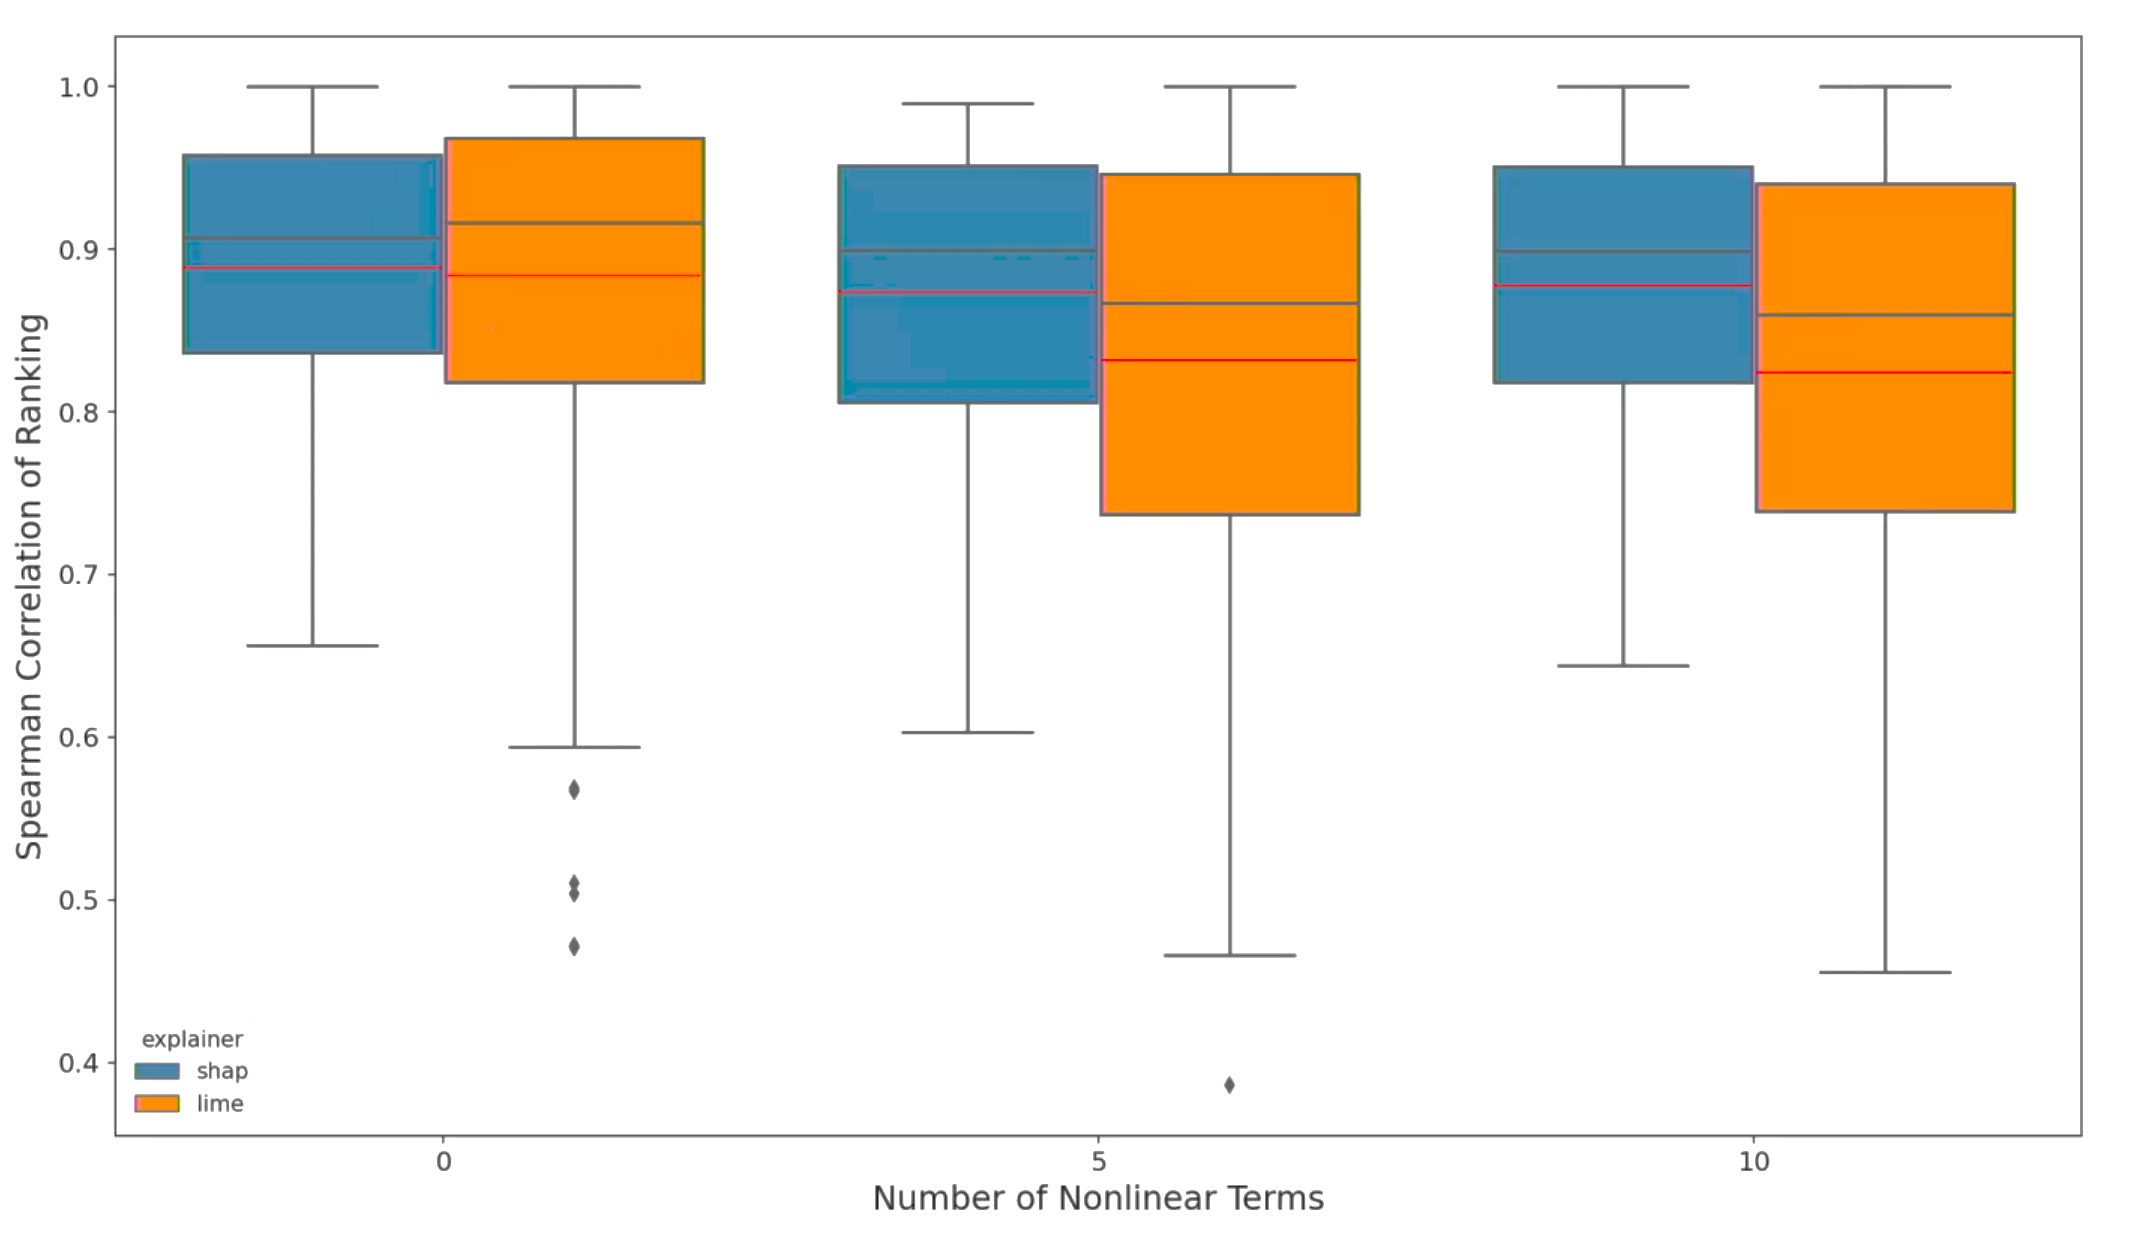
\includegraphics[width=0.45\textwidth]{media/image29.png}
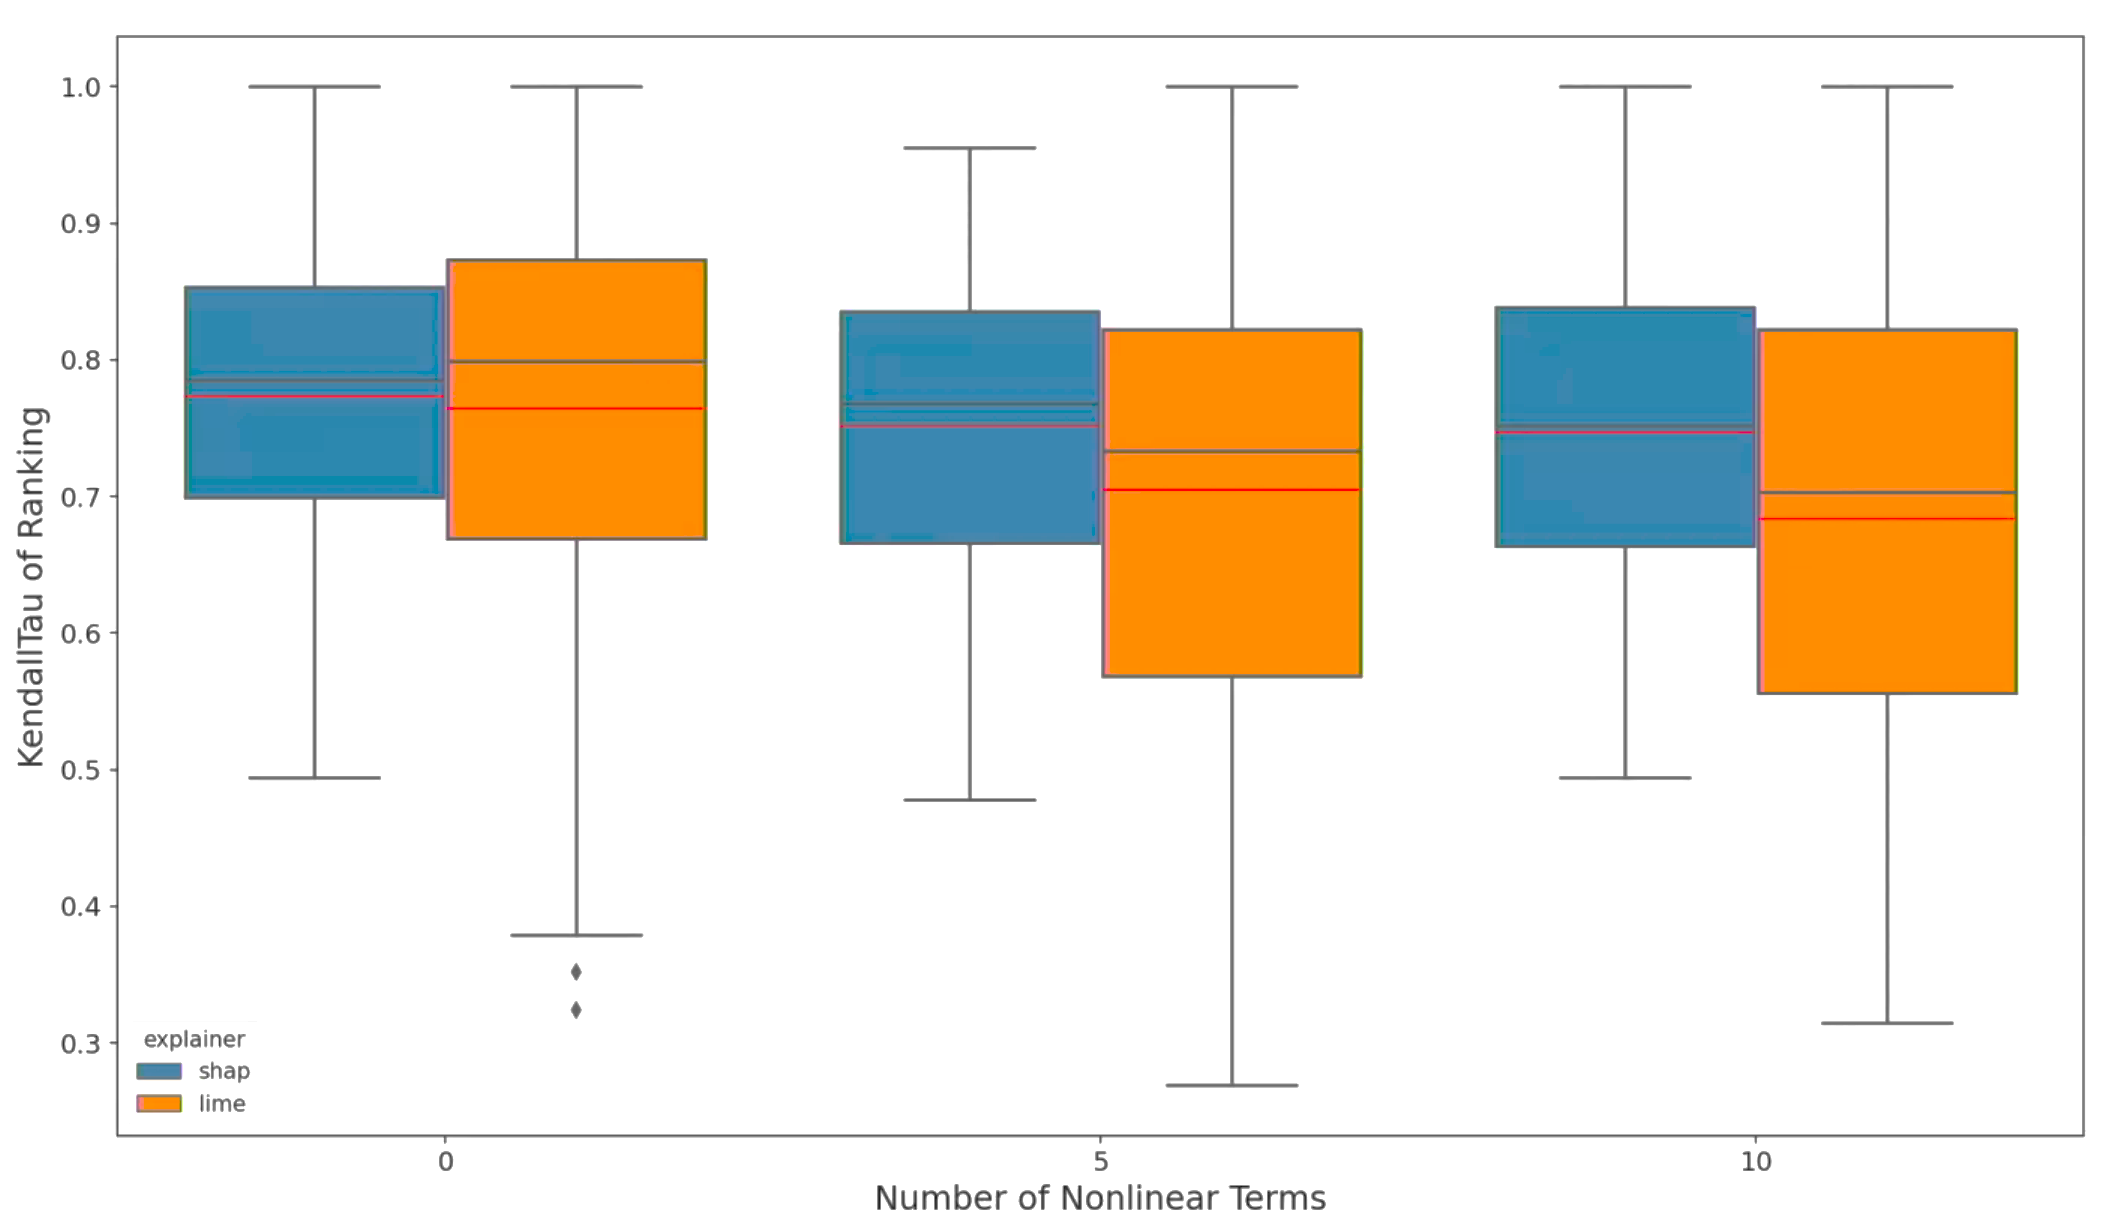
\includegraphics[width=0.45\textwidth]{media/image30.png}
\caption{Fig 17.1 Global Spearman Correlation of Explanations (LIME/SHAP) Ranking Between M and G Under Different Nonlinear Term Number (left) and Fig 17.2. Global Kendall Tau of Explanations (LIME/SHAP) Ranking Between M and G Under Different Nonlinear Term Number (right)}
\end{figure}

\begin{figure}[H]
\centering
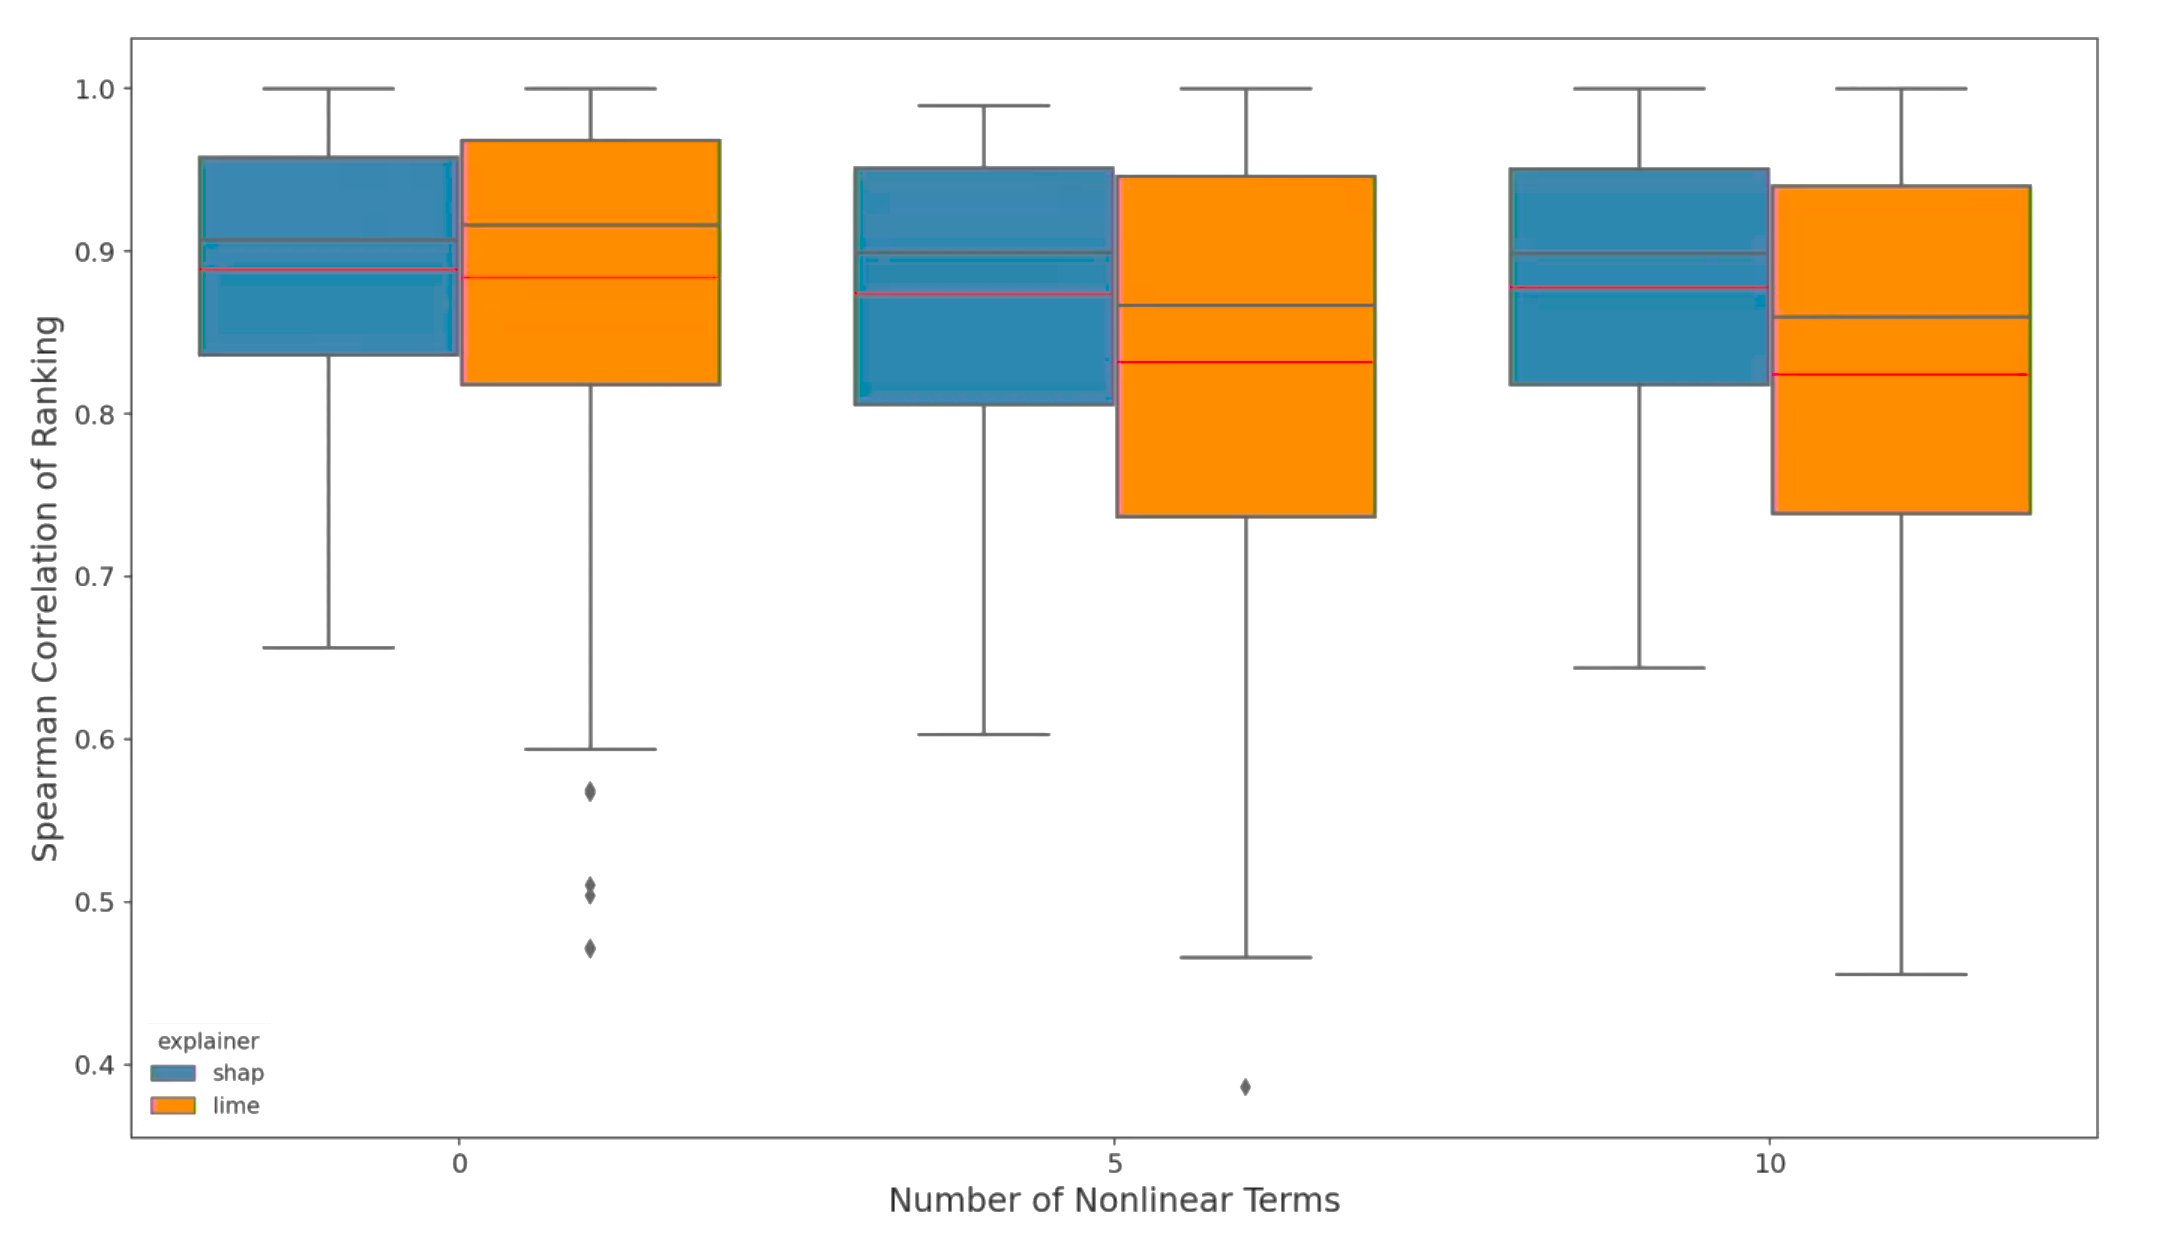
\includegraphics[width=0.45\textwidth]{media/image31.png}
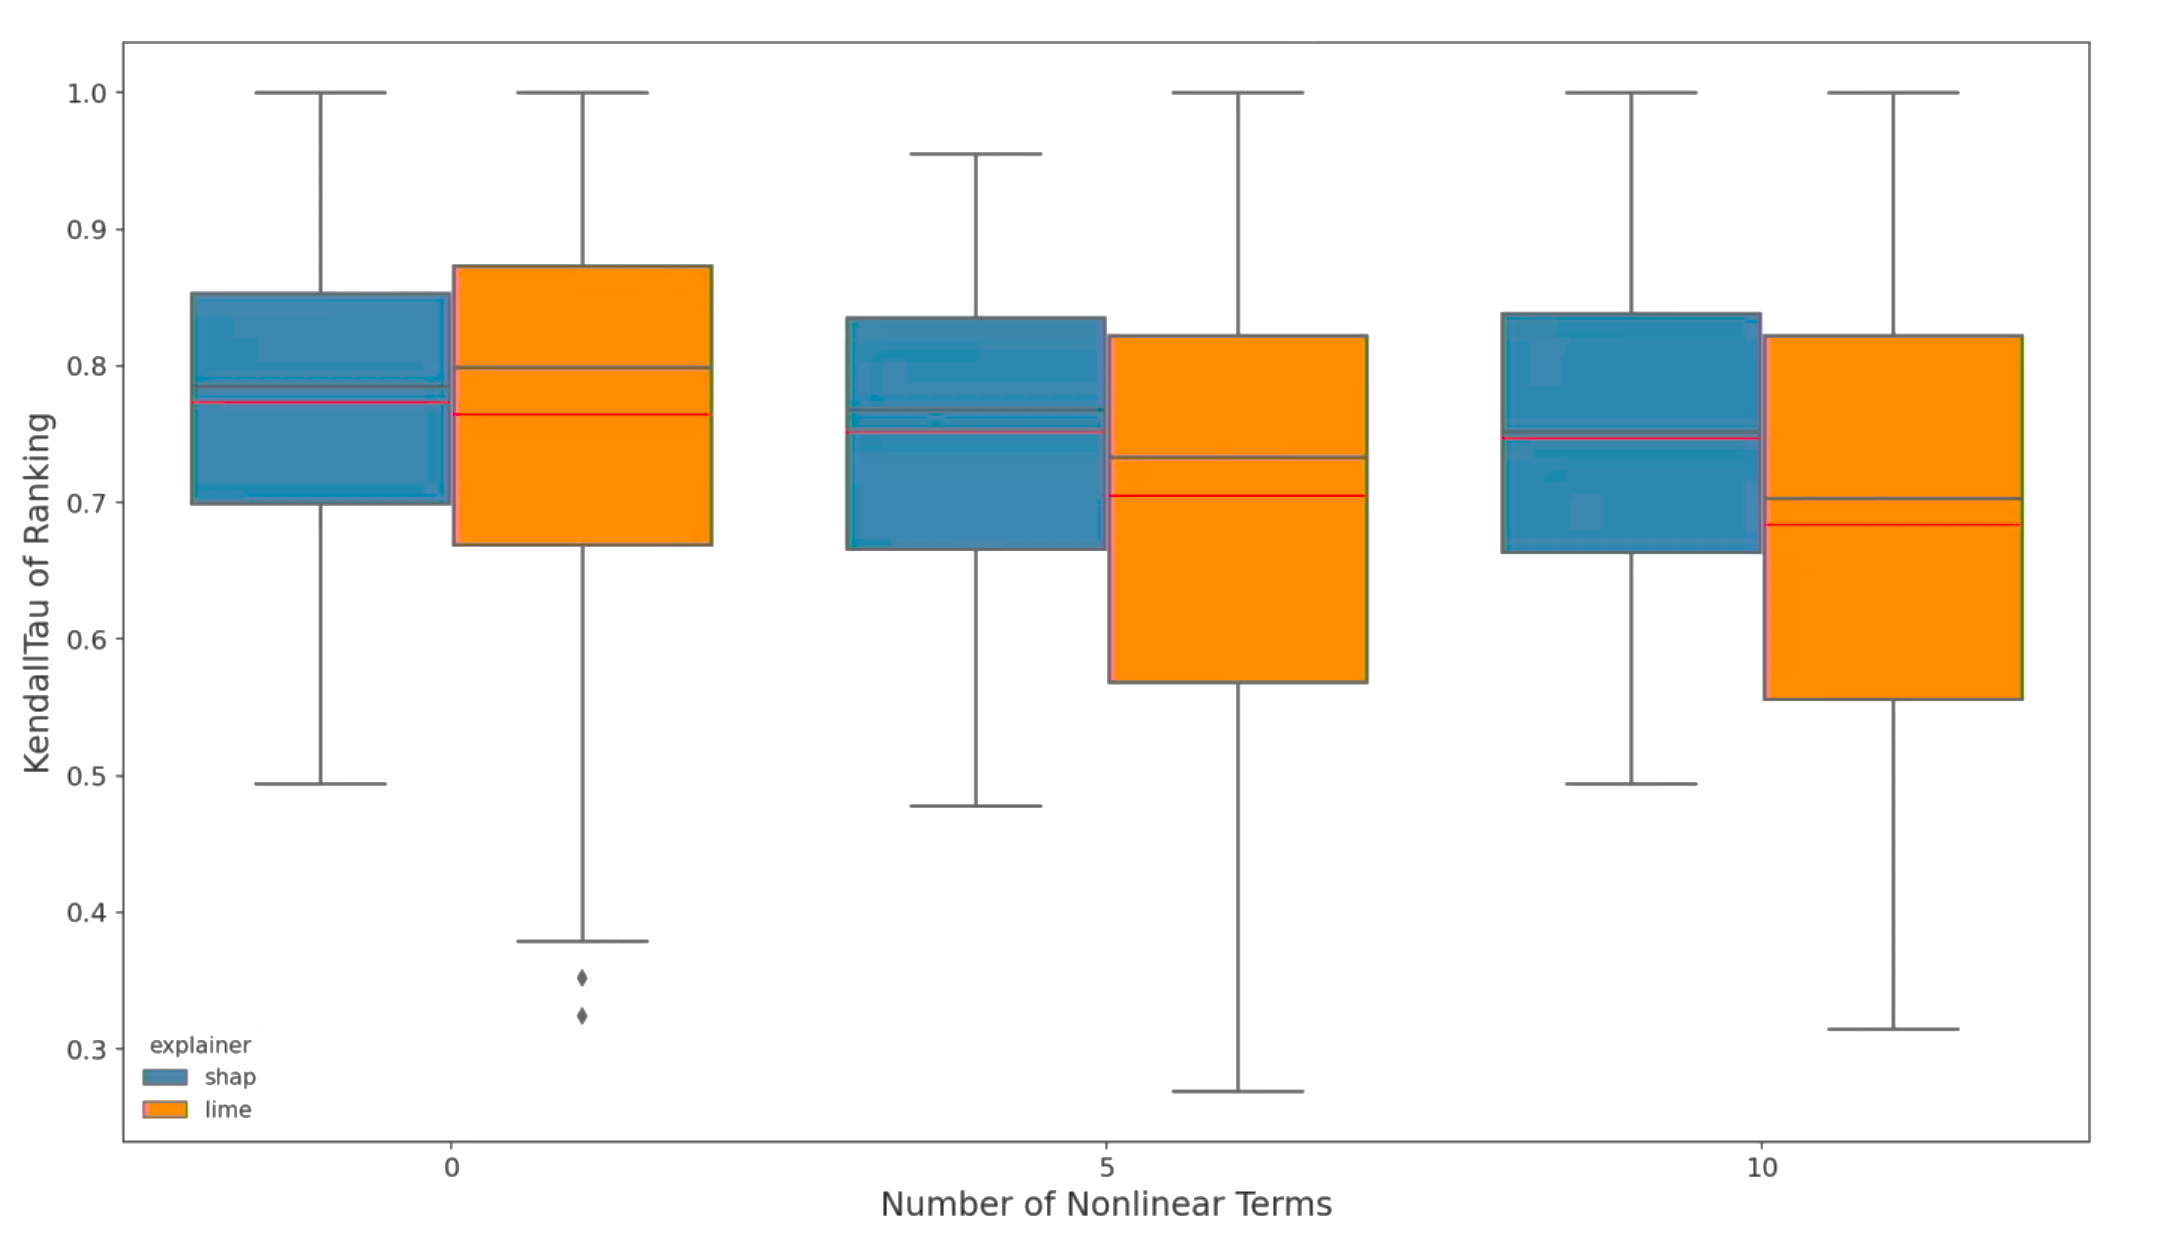
\includegraphics[width=0.45\textwidth]{media/image32.png}
\caption{Fig 18.1 Local Spearman Correlation of Explanations (LIME/SHAP) Ranking Between M and G Under Different Nonlinear Term Number (left) and Fig 18.2. Local Kendall Tau of Explanations (LIME/SHAP) Ranking Between M and G Under Different Nonlinear Term Number (right)}
\end{figure}

\begin{figure}[H]
\centering
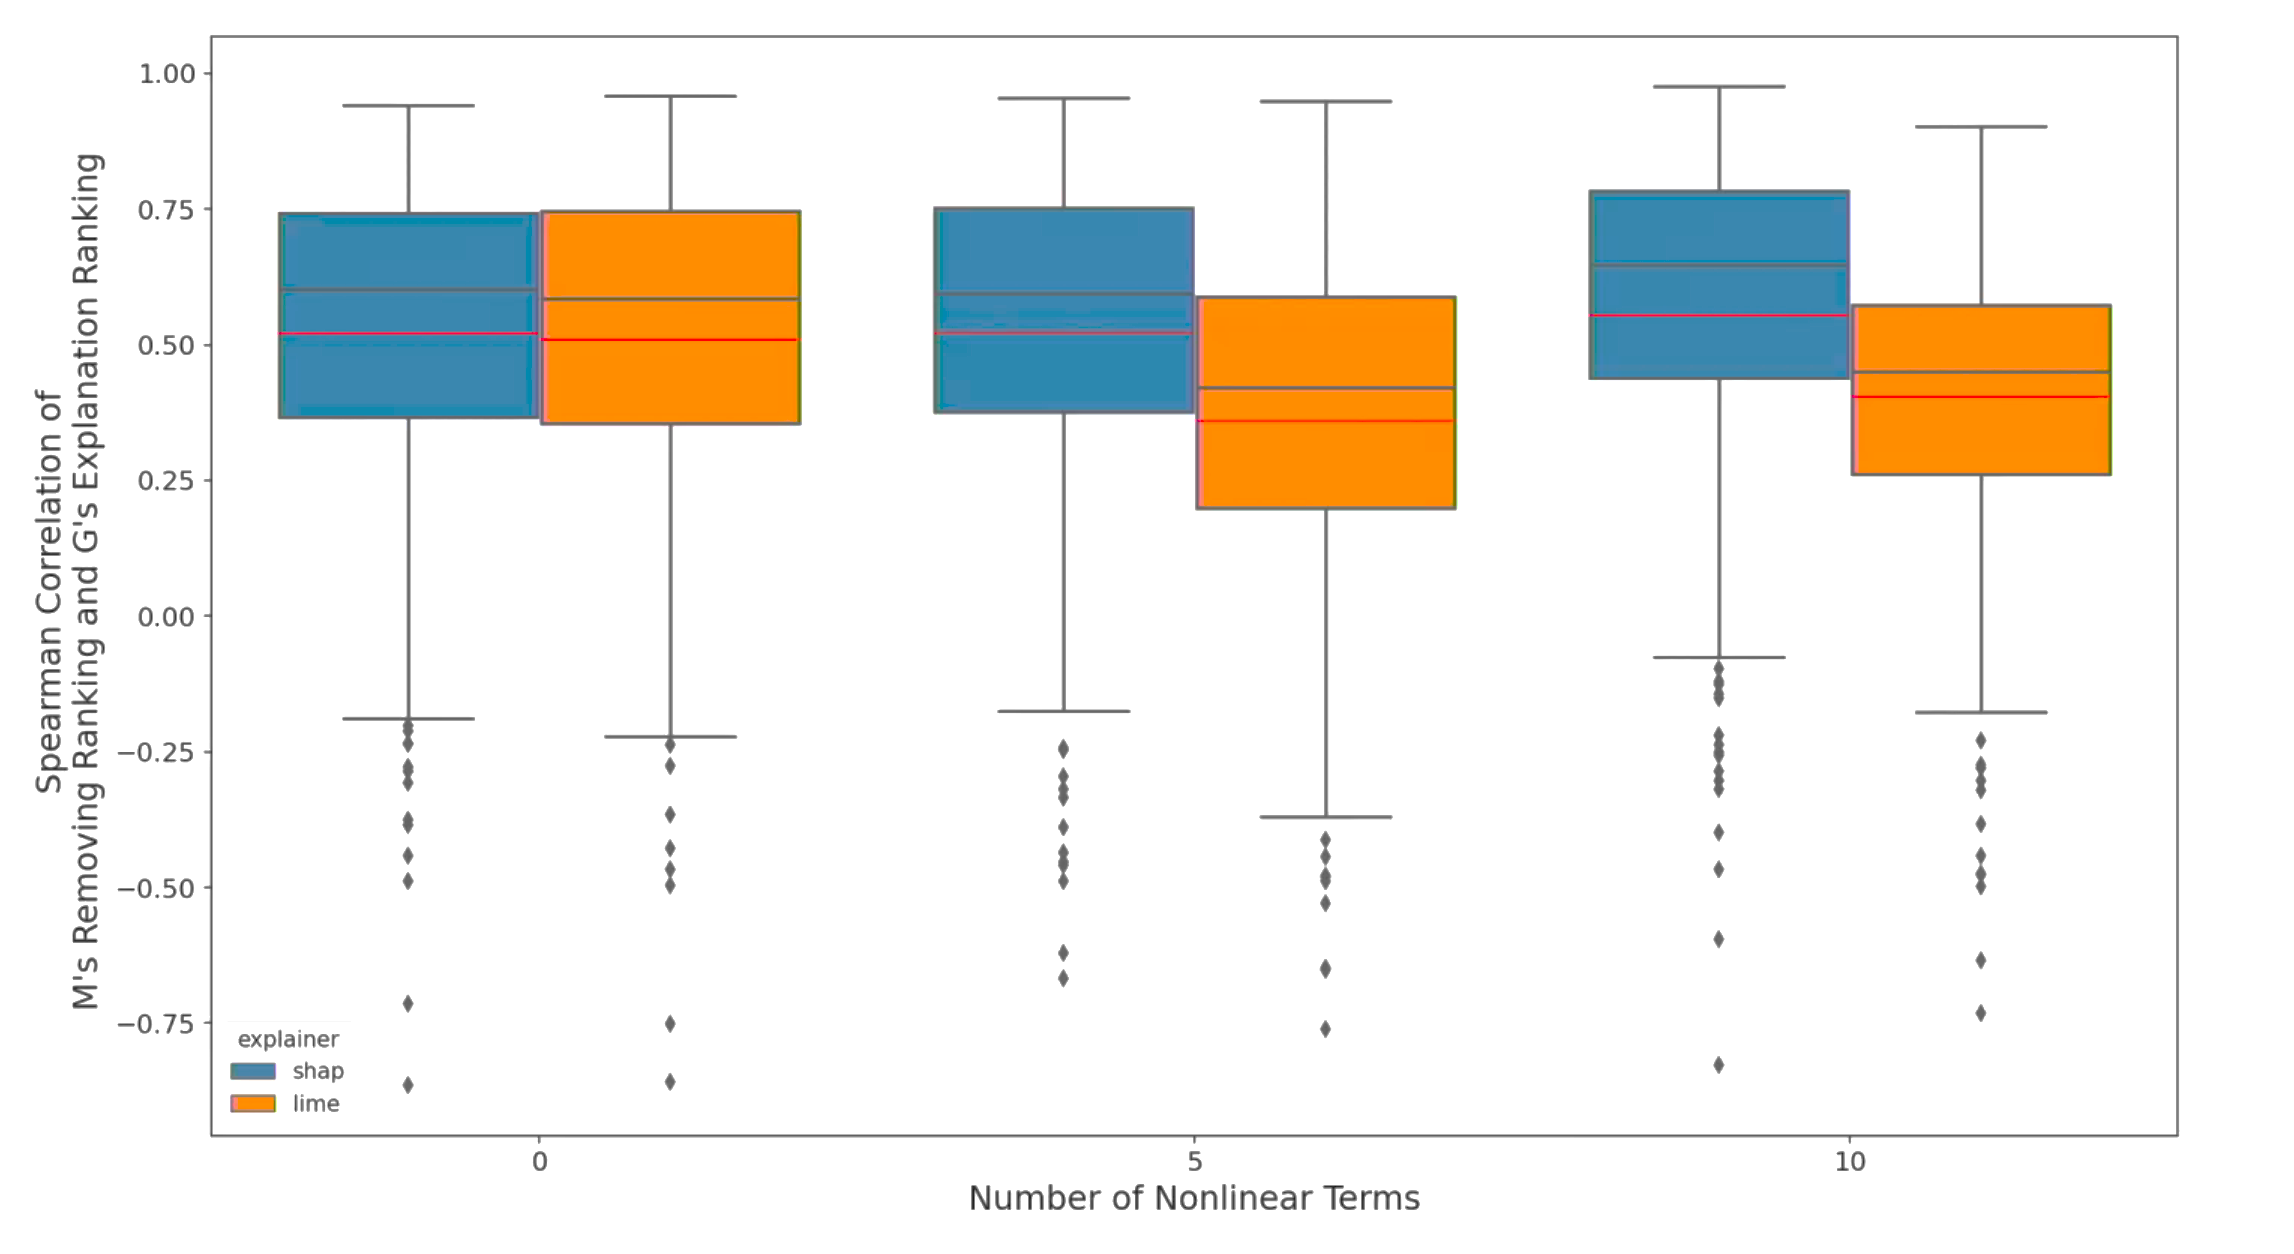
\includegraphics[width=0.45\textwidth]{media/image33.png}
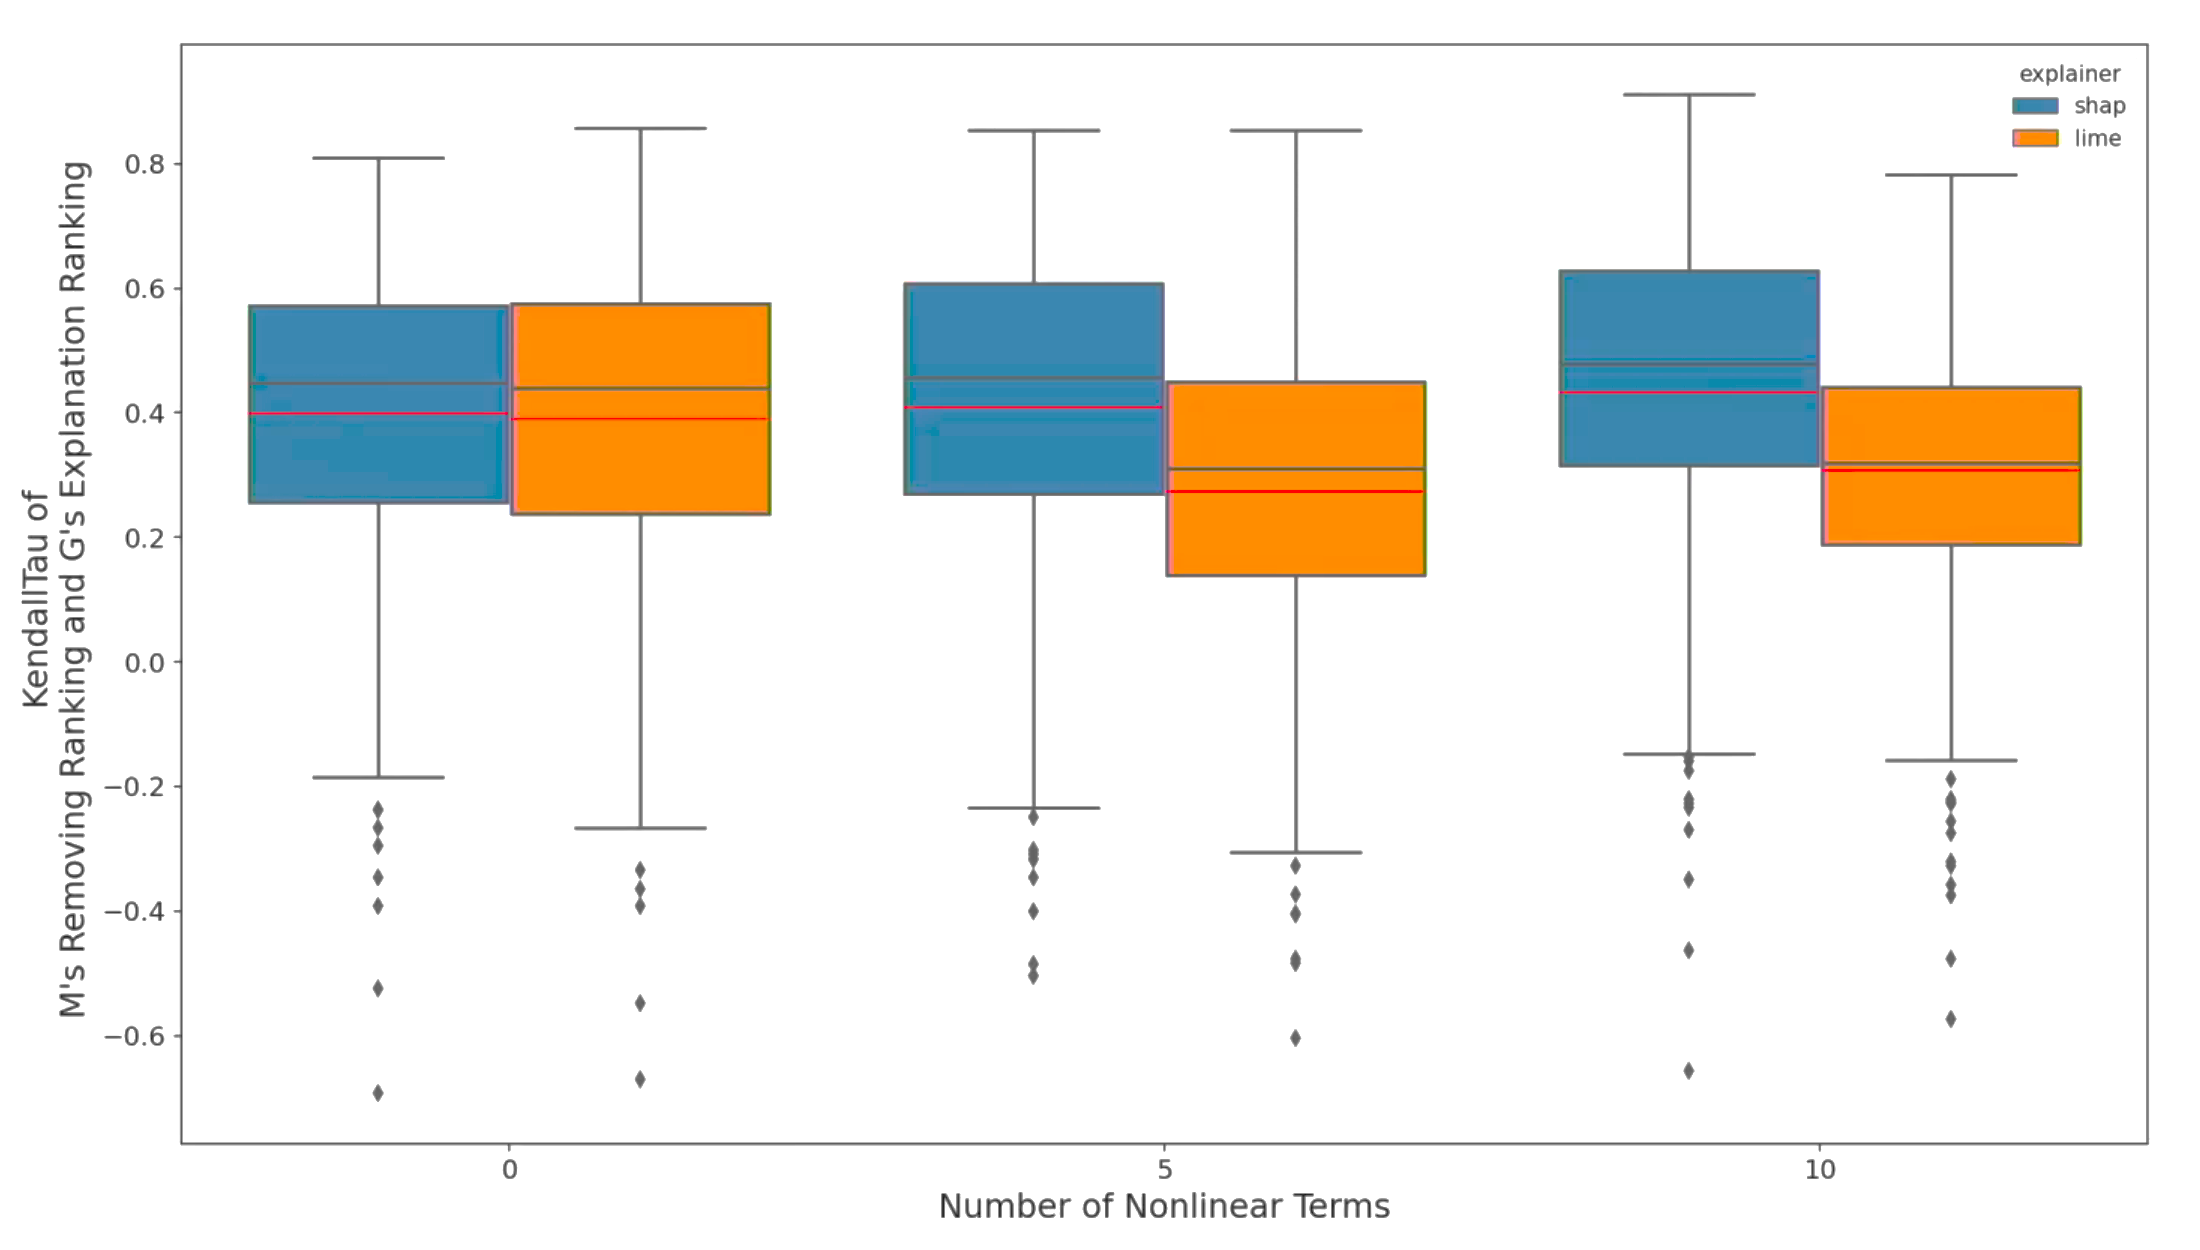
\includegraphics[width=0.45\textwidth]{media/image34.png}
\caption{Fig 19.1 Remove Ranking Spearman Correlation of Explanations (LIME/SHAP) Ranking Between M and G Under Different Nonlinear Term Number (left) and Fig 19.2. Remove Ranking Kendall Tau of Explanations (LIME/SHAP) Ranking Between M and G Under Different Nonlinear Term Number (right)}
\end{figure}

\begin{figure}[H]
\centering
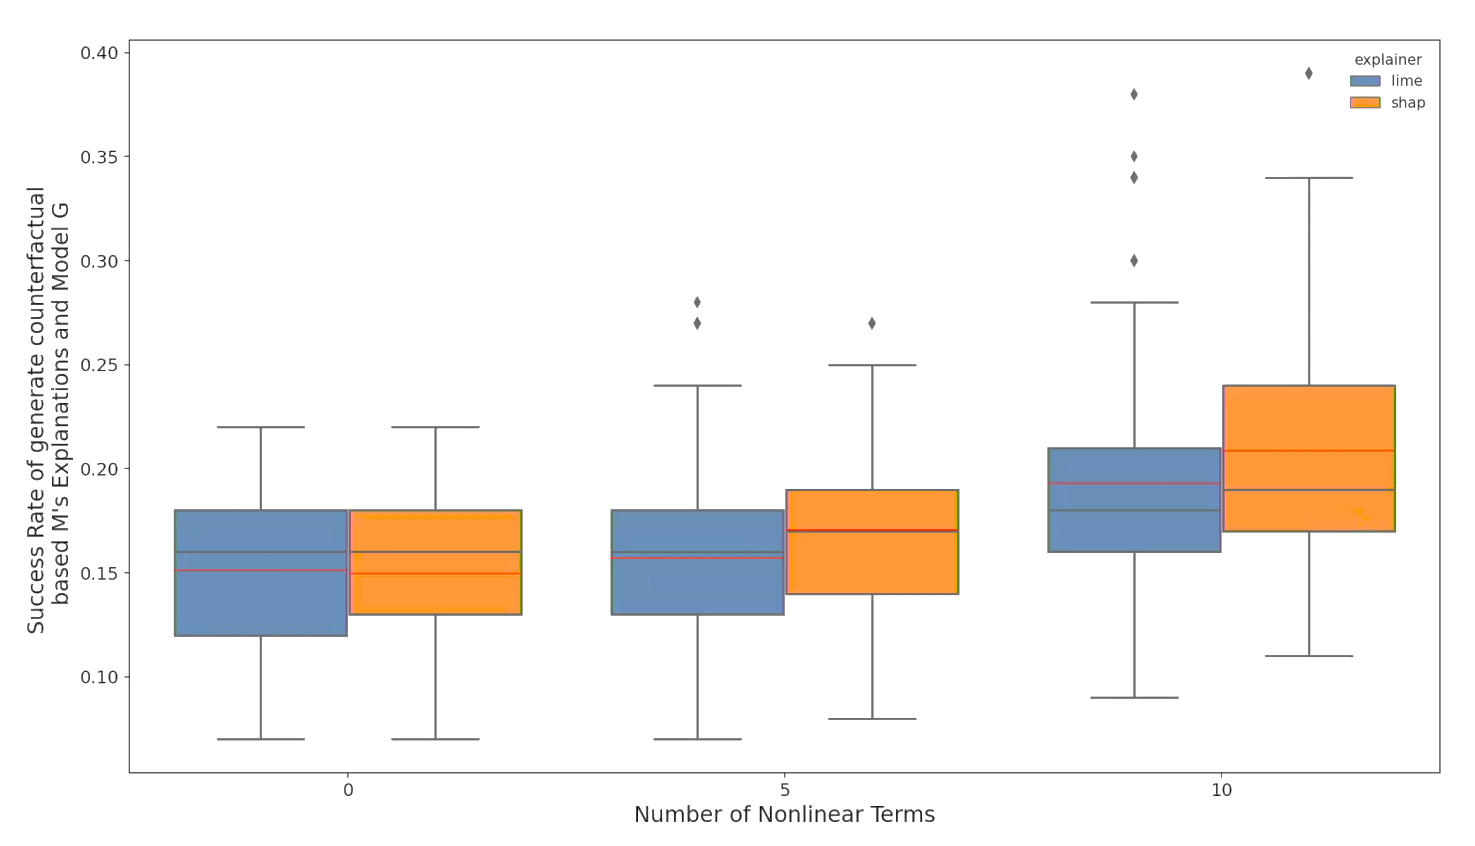
\includegraphics[width=0.7\textwidth]{media/image35.png}
\caption{Fig Success Rate of Generate Counterfactual based M's Explanations (LIME/SHAP) and Model G Under Different Nonlinear Term Number}
\end{figure}

\subsection{Results of Factor Regression}

\begin{figure}[H]
\centering
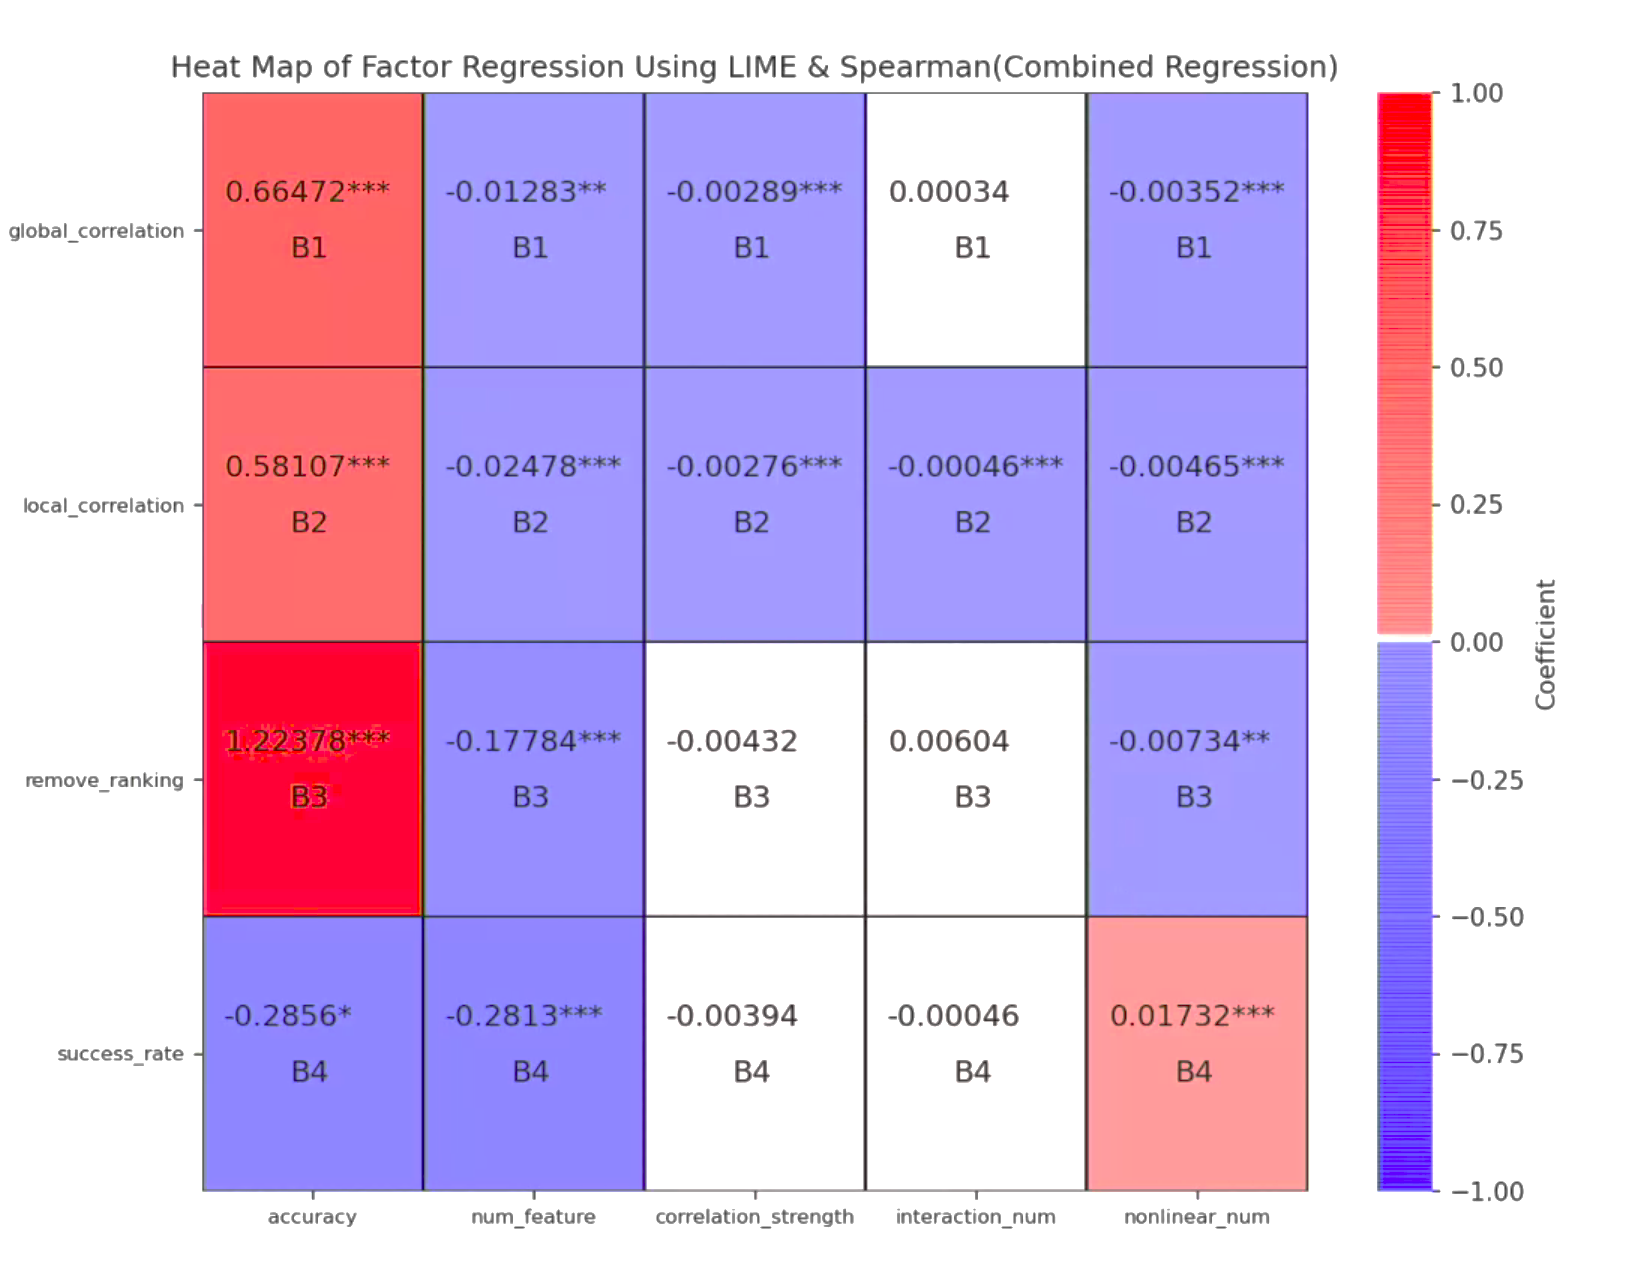
\includegraphics[width=0.8\textwidth]{media/image36.png}
\caption{Heat Map of Factor Regression Using LIME \& Spearman(Combined Regression)}
\end{figure}

\begin{figure}[H]
\centering
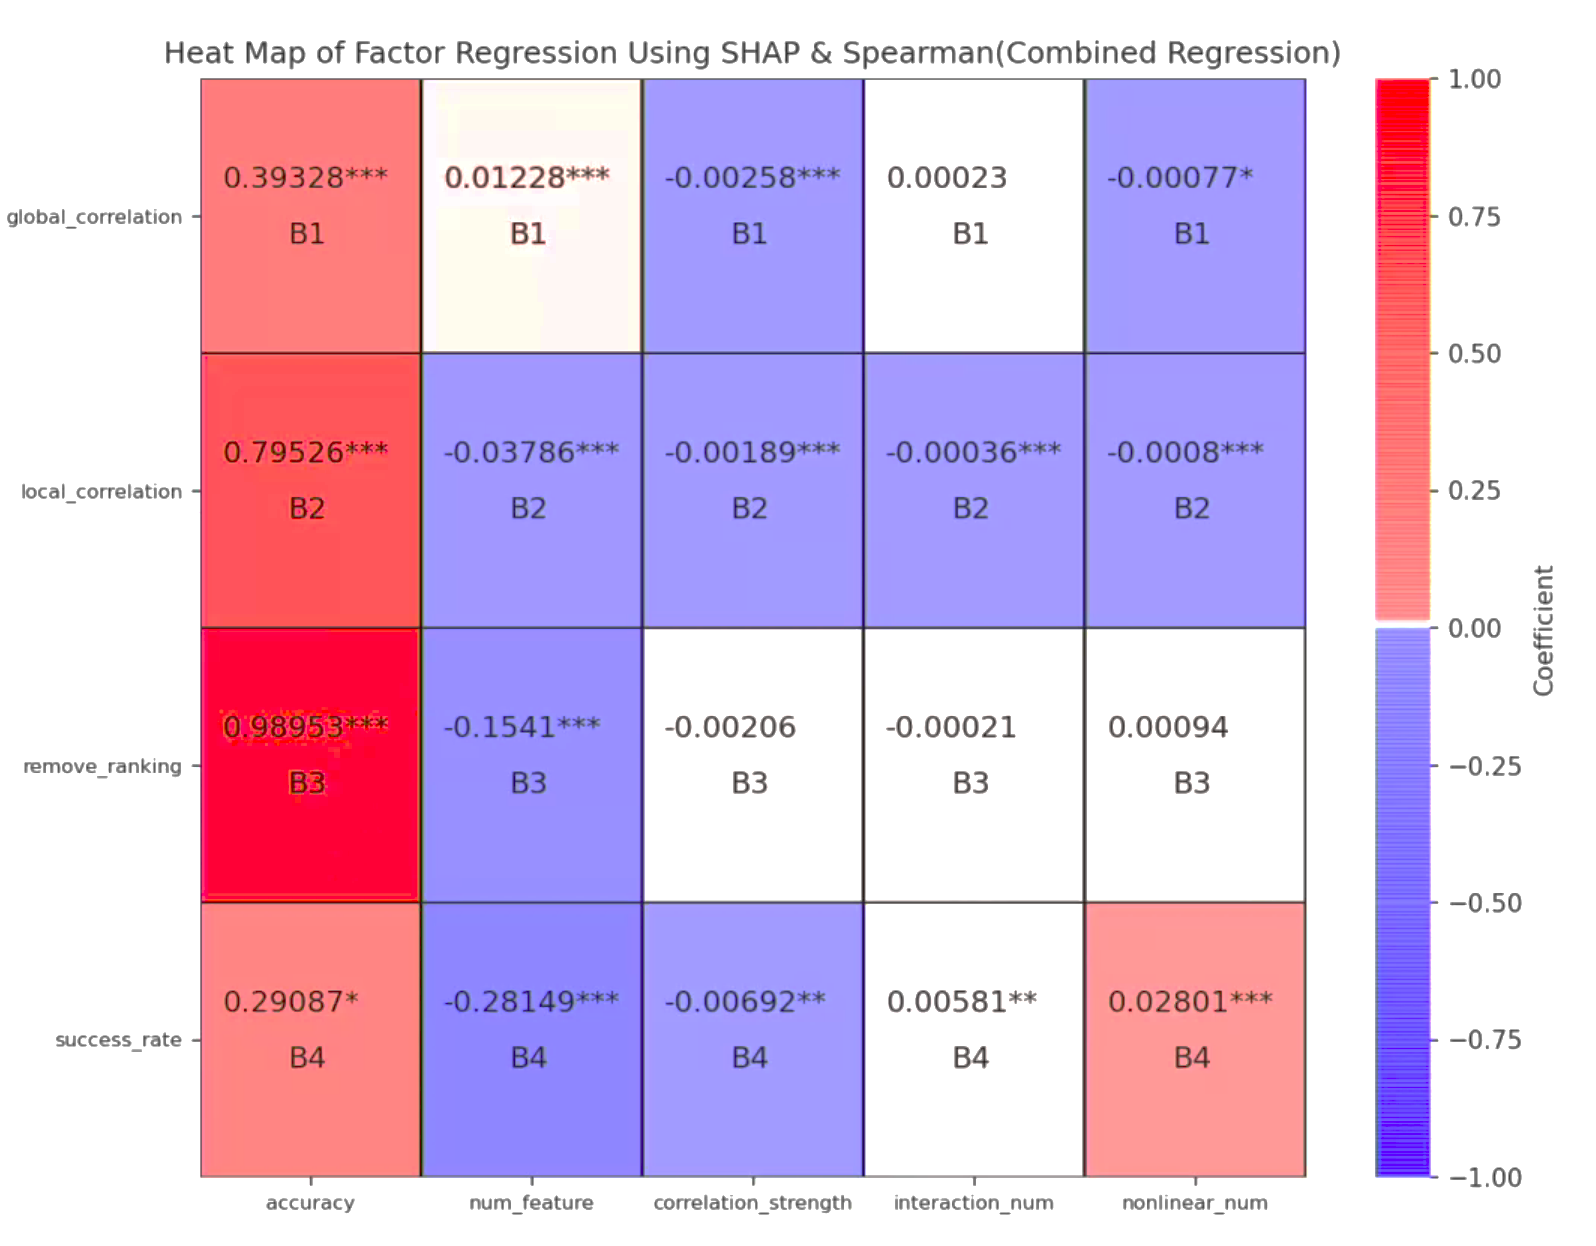
\includegraphics[width=0.8\textwidth]{media/image37.png}
\caption{Heat Map of Factor Regression Using SHAP \& Spearman(Combined Regression)}
\end{figure}

\begin{figure}[H]
\centering
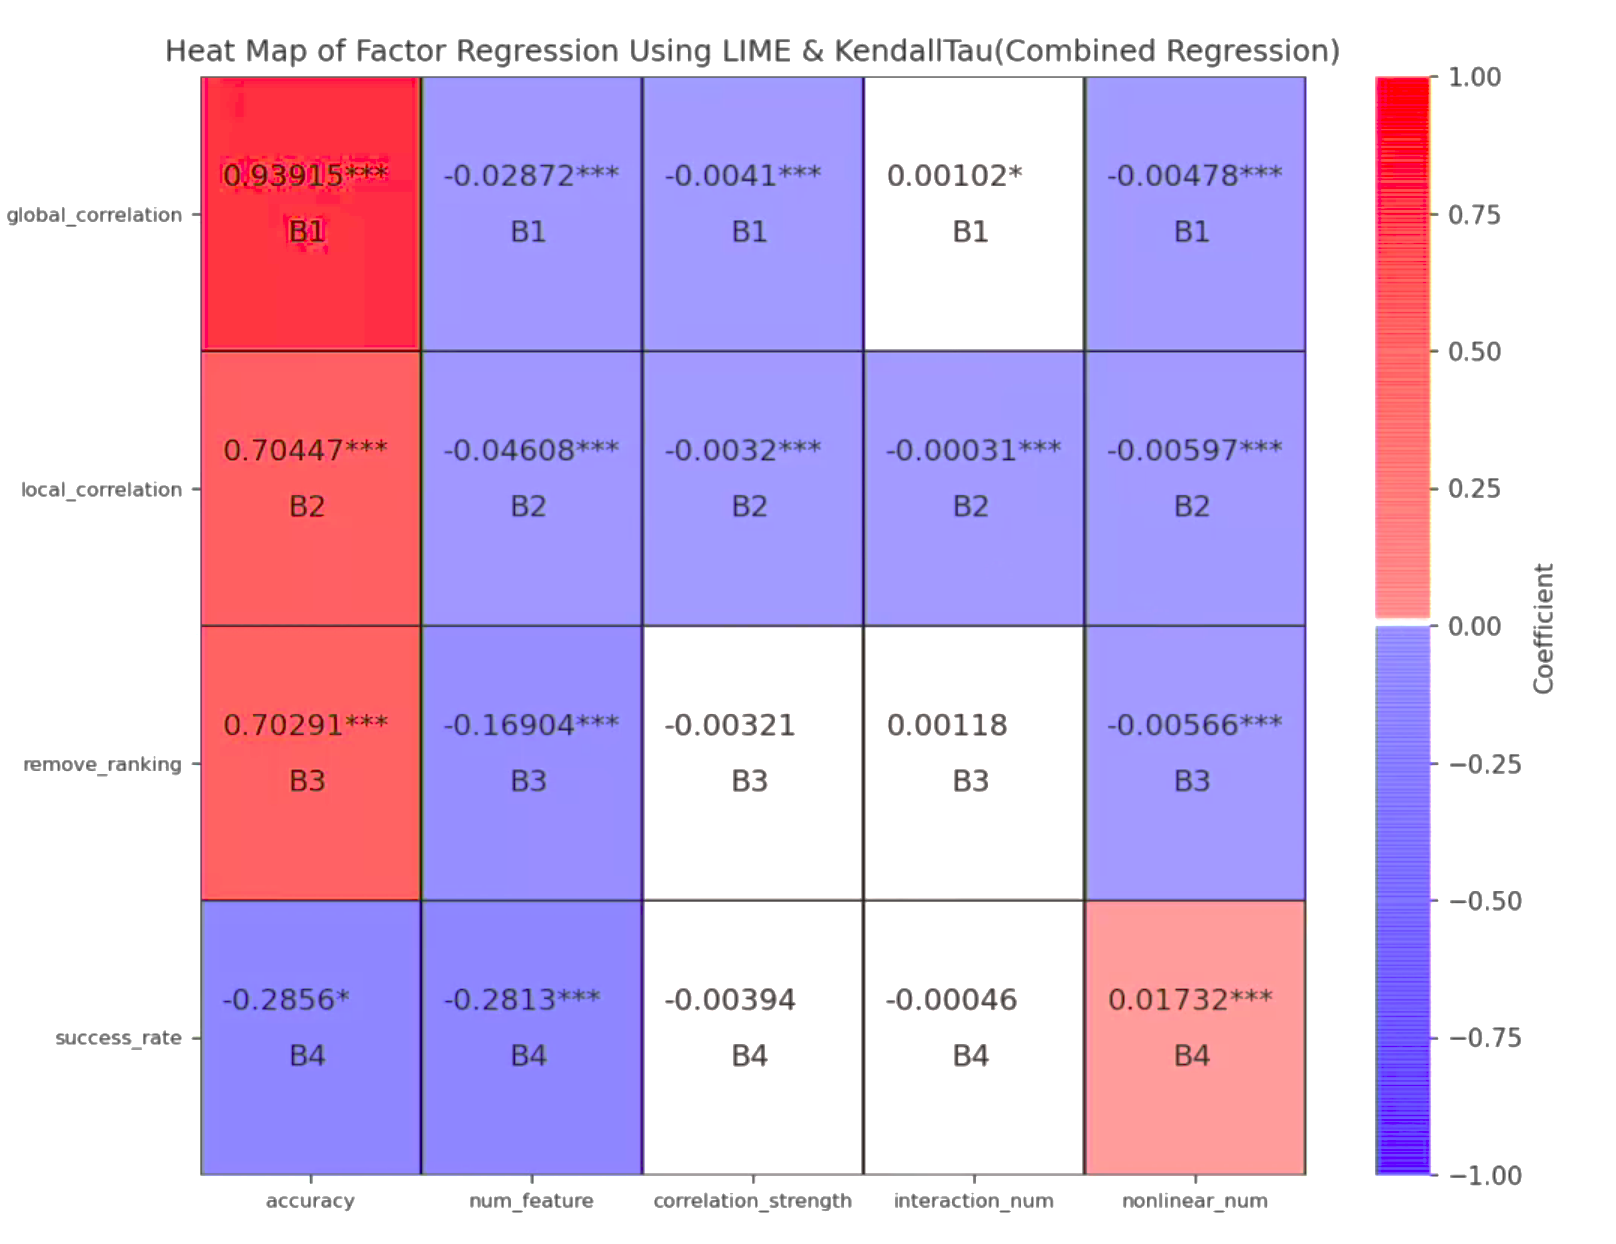
\includegraphics[width=0.8\textwidth]{media/image38.png}
\caption{Heat Map of Factor Regression Using LIME \& Spearman(Combined Regression)}
\end{figure}

\begin{figure}[H]
\centering
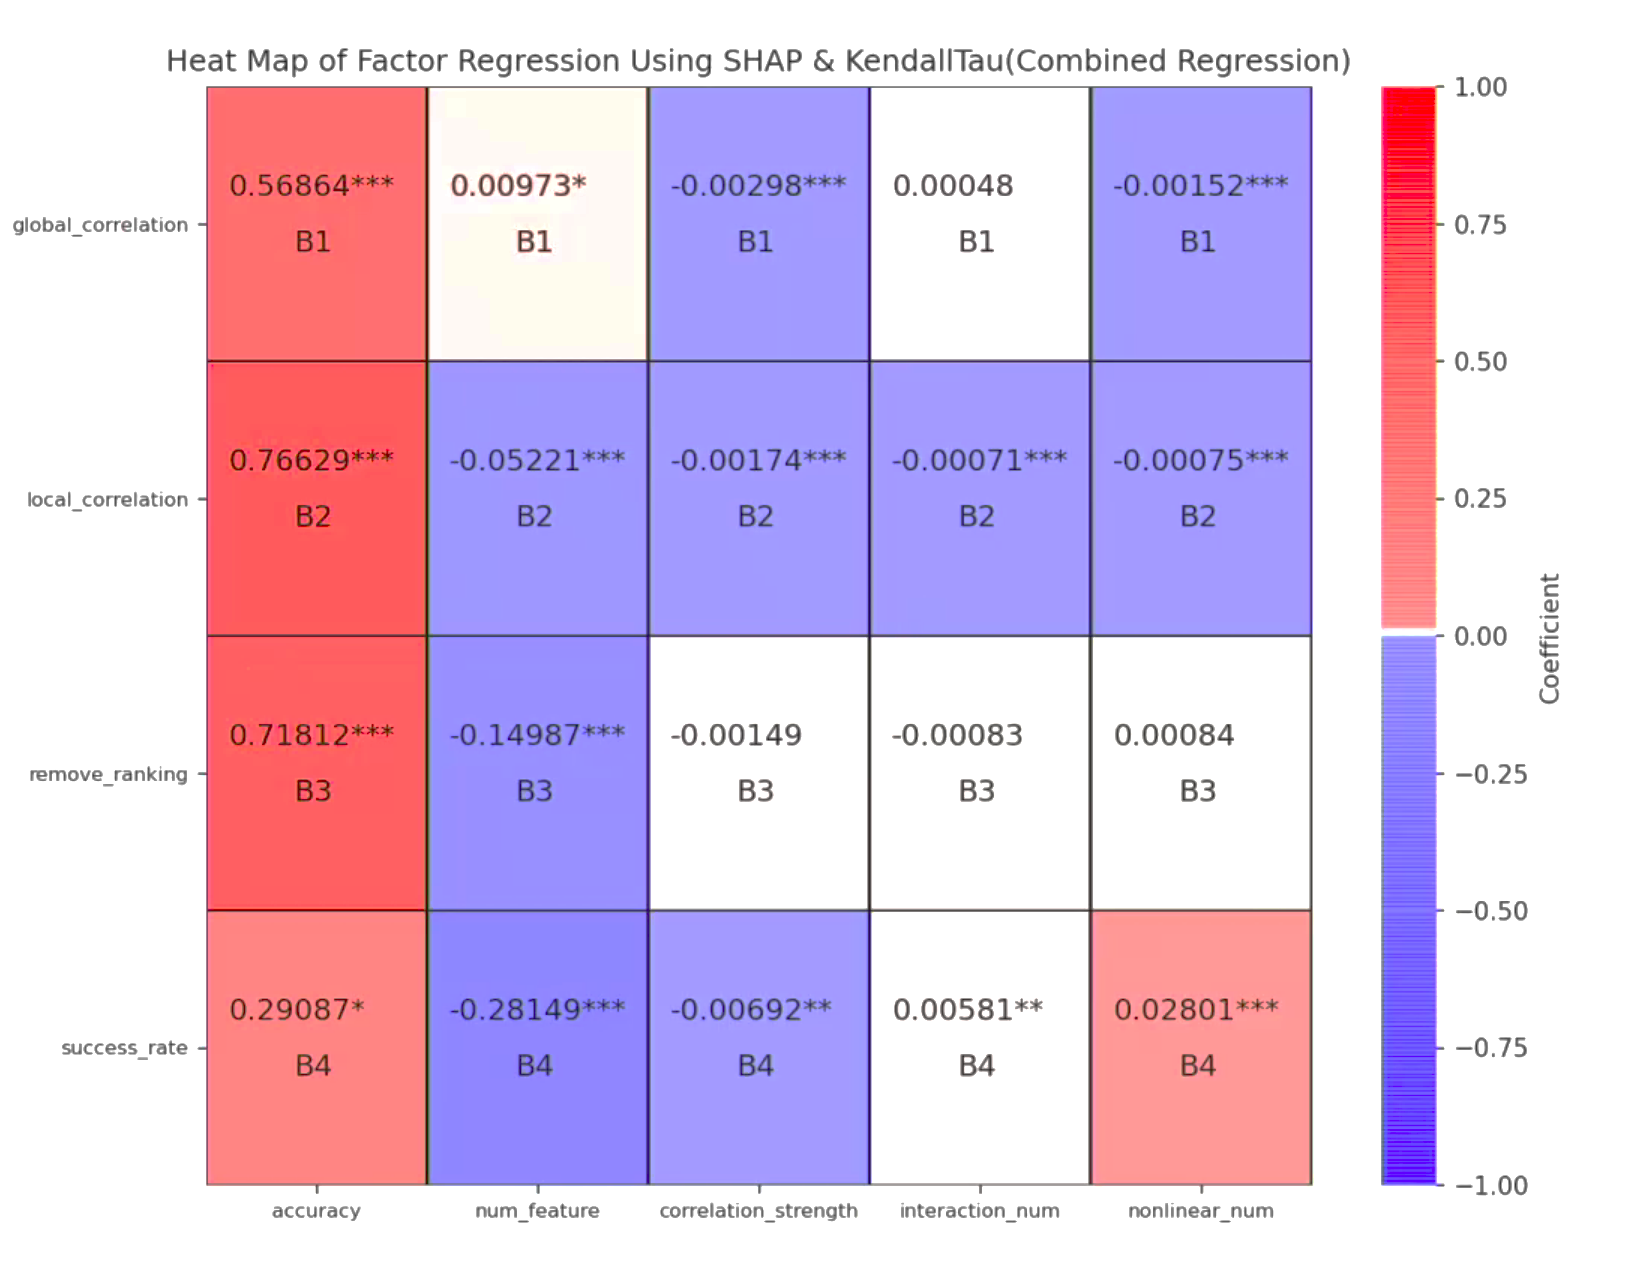
\includegraphics[width=0.8\textwidth]{media/image39.png}
\caption{Heat Map of Factor Regression Using SHAP \& Kendall Tau (Combined Regression)}
\end{figure}

\begin{landscape}
\begin{table}[H]
\centering
\caption{Factor Regression between all factors and Global Correlation}
\begin{tabular}{lcccc}
\toprule
 & (1) & (2) & (3) & (4) \\
 & LIME \& Spearman & SHAP \& Spearman & LIME \& Kendall Tau & SHAP \& Kendall Tau \\

Variables & log (Global Correlation) & log (Global Correlation) & log (Global Correlation) & log (Global Correlation) \\
\midrule
log (Accuracy) & 0.665*** & 0.393*** & 0.939*** & 0.569*** \\
 & (0.0278) & (0.0194) & (0.0320) & (0.0244) \\
log (Num\_feature) & -0.0128** & 0.0123*** & -0.0287*** & 0.0097* \\
 & (0.0041) & (0.0034) & (0.0055) & (0.0049) \\
log (Correlation\_strength) & -0.029*** & -0.0026*** & -0.0041*** & -0.003*** \\
 & (0.0005) & (0.0004) & (0.0007) & (0.0005) \\
log (Nonlinear\_num) & -0.035*** & -0.0008* & -0.0048*** & -0.0015*** \\
 & (0.0004) & (0.0003) & (0.0005) & (0.0004) \\
log (Interaction\_num) & 0.00034 & 0.00023 & 0.0010* & 0.0005 \\
 & (0.0004) & (0.0003) & (0.0005) & (0.0004) \\
Intercept & 0.785*** & 0.674*** & 0.814*** & 0.650*** \\
 & (0.0143) & (0.0109) & (0.0189) & (0.0162) \\
\midrule
R\textsuperscript{2} & 0.48 & 0.35 & 0.56 & 0.39 \\
Number of Models & 887 & 892 & 885 & 892 \\
\bottomrule
\multicolumn{5}{l}{Standard errors in parentheses} \\
\multicolumn{5}{l}{* $p<0.05$, ** $p<0.01$, *** $p<0.001$} \\
\end{tabular}
\end{table}
\end{landscape}

\begin{landscape}
\begin{table}[h]
\centering
\caption{Factor Regression between all factors and Local Correlation}
\begin{tabular}{lcccc}
\toprule
 & (1) & (2) & (3) & (4) \\
 & LIME \& Spearman & SHAP \& Spearman & LIME \& Kendall Tau & SHAP \& Kendall Tau \\

Variables & log (Local Correlation) & log (Local Correlation) & log (Local Correlation) & log (Local Correlation) \\
\midrule
log (Accuracy) & 0.581*** & 0.795*** & 0.704*** & 0.766*** \\
 & (0.0029) & (0.0053) & (0.0031) & (0.0046) \\
log (Num\_feature) & -0.0248*** & -0.038*** & -0.0046*** & -0.0522*** \\
 & (0.0004) & (0.00097) & (0.0005) & (0.0008) \\
log (Correlation\_strength) & -0.0028*** & -0.0019*** & -0.0032*** & -0.0017*** \\
 & (0.00006) & (0.00009) & (0.00007) & (0.00008) \\
log (Nonlinear\_num) & -0.0047*** & -0.0008*** & -0.0060*** & -0.0008*** \\
 & (0.00004) & (0.00007) & (0.00005) & (0.00006) \\
log (Interaction\_num) & -0.00046*** & 0.0036*** & 0.0003*** & -0.00071*** \\
 & (0.00004) & (0.00006) & (0.00005) & (0.00006) \\
Intercept & 0.774*** & 0.815*** & 0.771*** & 0.765*** \\
 & (0.0015) & (0.0026) & (0.0018) & (0.0024) \\
\midrule
R\textsuperscript{2} & 0.44 & 0.38 & 0.51 & 0.41 \\
Number of Instances & 84,562 & 71,362 & 83,780 & 71,076 \\
Number of Models & 887 & 892 & 885 & 892 \\
\bottomrule
\multicolumn{5}{l}{Standard errors in parentheses} \\
\multicolumn{5}{l}{* $p<0.05$, ** $p<0.01$, *** $p<0.001$} \\
\end{tabular}
\end{table}
\end{landscape}

\begin{landscape}
\begin{table}[H]
\centering
\caption{Factor Regression between all factors and Remove Ranking Correlation}
\begin{tabular}{lcccc}
\toprule
 & (1) & (2) & (3) & (4) \\
 & LIME \& Spearman & SHAP \& Spearman & LIME \& Kendall Tau & SHAP \& Kendall Tau \\

Variables & \makecell{log (Remove Ranking \\Correlation)} & \makecell{log (Remove Ranking \\Correlation)}) & \makecell{log (Remove Ranking \\Correlation)} & \makecell{log (Remove Ranking \\Correlation)} \\
\midrule
log (Accuracy) & 1.224*** & 0.990*** & 0.703*** & 0.718*** \\
 & (0.2510) & (0.2069) & (0.1723) & (0.1522) \\
log (Num\_feature) & -0.1778*** & 0.1541*** & -0.1690*** & -0.1499*** \\
 & (0.0280) & (0.0188) & (0.0161) & (0.0134) \\
log (Correlation\_strength) & -0.0043 & -0.0021 & -0.0032 & -0.0015 \\
 & (0.0033) & (0.0025) & (0.0022) & (0.0019) \\
log (Nonlinear\_num) & -0.0073** & 0.0009 & -0.0056*** & 0.0008 \\
 & (0.0026) & (0.0020) & (0.0017) & (0.0015) \\
log (Interaction\_num) & 0.0060 & -0.0002 & 0.0012 & -0.0008 \\
 & (0.0031) & (0.0021) & (0.0020) & (0.0015) \\
Intercept & 1.210*** & 1.150*** & 1.005*** & 0.999*** \\
 & (0.1155) & (0.0880) & (0.0736) & (0.0617) \\
\midrule
R\textsuperscript{2} & 0.18 & 0.17 & 0.23 & 0.22 \\
Number of Models & 509 & 661 & 504 & 648 \\
\bottomrule
\multicolumn{5}{l}{Standard errors in parentheses} \\
\multicolumn{5}{l}{* $p<0.05$, ** $p<0.01$, *** $p<0.001$} \\
\end{tabular}
\end{table}
\end{landscape}

\begin{table}[h]
\centering
\caption{Factor Regression between all factors and Success Rate}
\begin{tabular}{lcc}
\toprule
 & (1) & (2) \\
 & LIME & SHAP \\

Variables & log (Success rate) & log (Success rate) \\
\midrule
log (Accuracy) & 0.0026 & 0.0026 \\
 & (0.085) & (0.0851) \\
log (Num\_feature) & -0.2814*** & -0.2814*** \\
 & (0.0140) & (0.0140) \\
log (Correlation\_strength) & -0.0054*** & -0.0054*** \\
 & (0.0020) & (0.0020) \\
log (Nonlinear\_num) & -0.0227*** & -0.0227*** \\
 & (0.0014) & (0.0014) \\
log (Interaction\_num) & 0.0027 & 0.0027 \\
 & (0.0015) & (0.0015) \\
Intercept & -0.971*** & -0.971*** \\
 & (0.0454) & (0.0454) \\
\midrule
R\textsuperscript{2} & 0.28 & 0.28 \\
Number of Models & 1,922 & 1,922 \\
\bottomrule
\multicolumn{3}{l}{Standard errors in parentheses} \\
\multicolumn{3}{l}{* $p<0.05$, ** $p<0.01$, *** $p<0.001$} \\
\end{tabular}
\end{table}
\end{document}